%!TEX root = 3-P_Masterdokument.tex
%!TEX encoding = UTF-8 Unicode

\chapter{Minor word classes}\label{chap:MinorWordClasses}

The major word classes in Paunaka can be considered nouns and verbs, just like in many other languages around the world. They are large and open and described in detail in Chapters \ref{chapter:Nouns} and \ref{sec:Verbs}, respectively.

There are, however, also minor word classes, minor in the sense that they are rather small, with considerably fewer members. Only one of them can be considered absolutely closed, this is the pronouns and nominal demonstratives (§\ref{chapter:Pronouns}). Adpositions can also be considered a fairly closed class (see \sectref{sec:Adpositions}). Among adjectives, numerals, and quantifiers (\sectref{sec:AdjectivesNumerals}), adverbs (\sectref{sec:Adverbs}), and connectives (\sectref{sec:Conjunctions}), however, we find loans\is{borrowing} from Spanish and Bésiro, which shows that these classes are open for new members.


\section{Pronouns and nominal demonstratives}\label{chapter:Pronouns}
\is{pronoun|(}

This section covers pronouns, i.e. personal and topic pronouns, and also nominal demonstratives. It also deals with indefinite pronouns, which occur only rarely in Paunaka discourse. There are personal pronouns for first and second person singular and plural, but not for the third person. (\getref{ex:new23-biti}) includes the first person plural pronoun\is{personal pronoun} \textit{biti}. It comes from Juan Ch. talking about the the different types of work he and the other workers do for their \textit{patrón}.

\ea\label{ex:new23-biti}
\begingl
\glpreamble biti bisu\\
\gla biti bi-isu\\
\glb 1\textsc{pl.prn} 1\textsc{pl}-weed\\
\glft ‘we weed’
\endgl
\trailingcitation{[nxx-p630101g-1.089]}
\xe

In reference to a third person, a topic or demonstrative pronoun\is{nominal demonstrative} can be used instead. Topic pronouns\is{topic pronoun} are used in constructions that involve emphasis, more precisely \isi{topicalisation} (this being reflected in the name chosen for this pronoun) or \isi{focus}. (\getref{ex:new23-chibu}) comes from Miguel.\footnote{Note that this recording has not been archived because it contains sensitive data.}

\ea\label{ex:new23-chibu}
\begingl
\glpreamble chibu tikechunube\\
\gla chibu ti-kechu-nube\\
\glb 3\textsc{top.prn} 3i-say-\textsc{pl}\\
\glft ‘this is what they say’
\endgl
\trailingcitation{[jmx-c120429ls-x5.302]}
\xe

Paunaka has no articles, demonstrative pronouns\is{nominal demonstrative} preceding a noun are predominantly used to mark \isi{definiteness}, as far as I can tell. Nonetheless, just like other pronouns, demonstrative pronoun can occur on their own as well, as in (\getref{ex:new23-echÿu}) from Juana.

\ea\label{ex:new23-echÿu}
\begingl
\glpreamble entonses kuina tamicha echÿu\\
\gla entonses kuina ti-a-micha echÿu\\
\glb thus \textsc{neg} 3i-\textsc{irr}-be.good \textsc{dem}b\\
\glft ‘thus this is not good’
\endgl
\trailingcitation{[jmx-c120429ls-x5.199]}
\xe

There are certain overlaps in the composition of pronouns and nominal demonstratives.\is{nominal demonstrative} These overlaps also include the demonstrative adverbs\is{adverb!demonstrative adverb}\is{demonstrative!demonstrative adverb} and are illustrated in \figref{fig:PronounDemComposition}.

\begin{figure}
\fittable{
\begin{tabular}{|c|c|r|c|l|c|l|}
\multicolumn{1}{c}{Category} & \multicolumn{1}{c}{} & \multicolumn{3}{c}{Composition} & \multicolumn{1}{c}{} & \multicolumn{1}{c}{Rough translation}\cr
\cline{1-1} \cline{3-3} \cline{5-5} \cline{7-7}
\multirow{4}{*}{personal pronouns} && nÿ & + & ti && I\cr
&& pi & + & ti && you (\textsc{sg})\cr
&& bi & + & ti && we\cr
&& e & + & ti && you (\textsc{pl})\cr
\cline{1-1} \cline{5-5}
\multirow{2}{*}{topic pronouns} && chi & + & bu && he, she, it, this\cr
\cline{3-3}
&& ne & + & bu && there\cr
\cline{1-1} \cline{5-5}
nominal/adverbial demonstrative && ne & + & chÿ+u & & there\cr
\cline{1-1} \cline{3-3}
\multirow{2}{*}{nominal demonstratives} && e & + & chÿ+u & & the, this, that\cr
 \cline{5-5}
 && e & + & ka & & the, this, that\cr
 \cline{1-1} \cline{3-3}
 \multirow{2}{*}{adverbial demonstratives} && na & + & ka & & here\cr
 \cline{5-5}
 && na & + & uku & & there\cr
 \cline{1-1} \cline{3-3} \cline{5-5} \cline{7-7}
\end{tabular}
}

\captionof{figure}{The composition of personal and topic pronouns and demonstratives}
\label{fig:PronounDemComposition}
\end{figure}

\largerpage
The figure shows that personal pronouns consist of a person marker\is{person marking} (\textit{nÿ-, pi-, \mbox{bi-,} e-}) and a suffix \textit{-ti}. There is no third person personal pronoun with an analogous structure, but just like the personal pronouns, \textit{chibu} has a person marker in first position, the third person marker \textit{chÿ-} or \textit{chi-}. In this case, however, a different suffix is added, which is \mbox{\textit{-bu}}. This suffix also occurs on \textit{nebu}, the oblique variant of the topic pronoun (though with a somewhat restricted use). The prefix \textit{ne-} is also found on \textit{nechÿu}, which is analysed as demonstrative with nominal and adverbial\is{adverb!demonstrative adverb|(}\is{demonstrative!demonstrative adverb|(}\is{nominal demonstrative|(} function. It shares with the nominal demonstrative \textit{echÿu} that both end in \textit{-chÿ-u}. \textit{Echÿu} has in common with the other nominal demonstrative \textit{eka} that they both begin with \textit{e-}, while both \textit{eka} and \textit{naka}, the latter being the proximal demonstrative adverb, end in \textit{-ka}. The other demonstrative adverb is \textit{nauku}. This one also starts with \textit{na-}, it ends in \textit{-uku}.\is{nominal demonstrative|)}\is{demonstrative!demonstrative adverb|)}\is{adverb!demonstrative adverb|)} A suffix \textit{-uku} can be attached to personal pronouns to predicate location (see (\getref{ex:PersP-loc}) below) and this is where the circle closes.

In addition to the words given in \figref{fig:PronounDemComposition}, there is a negative third person pronoun,\is{pronoun!negative pronoun}\is{negation!negative pronoun} which is \textit{chÿina}. It alternates with \textit{chibu} and is thus described in the section on topic pronouns. There are also some additional deictic words that seem to build on the prefix \textit{ne-}, but they are described elsewhere: for \textit{nechikue} ‘therefore, that’s why’ see \sectref{sec:Conjunctions}, and for \textit{nena} ‘(be) like/similar to, resemble’ see \sectref{sec:SimilativePreds}. 

The overlap in composition does not include the indefinite pronouns \textit{chija} ‘something, someone’ and \textit{juchubu} ‘somewhere’, which originated from the identical question words \textit{chija} ‘what, who’ and \textit{juchubu} ‘where’.

\largerpage
\subsection{Personal pronouns}\label{sec:PersPron}
\is{personal pronoun|(}

As noted above, the personal pronouns are composed of the person markers\is{person marking} (see \sectref{sec:NumberPersonVerbs} and \sectref{sec:Possession}) and a syllable \textit{ti}, which is probably related to the non-possessed marker \textit{-ti} (see \sectref{sec:Inalienables}). This process is also found in the other Bolivian Arawakan languages\is{Southern Arawakan} \citep[503]{Danielsen2011}. In general, personal pronouns closely resemble the ones found in the other Bolivian Arawakan languages and to a lesser degree also those found in more distantly related Arawakan languages \citep[cf.][]{Danielsen2011}. 

There is no third person pronoun, but a \isi{topic pronoun} (see \sectref{sec:FocPron}) or \isi{nominal demonstrative} (see \sectref{sec:DemPron}) can be used instead. All personal pronouns are listed in \tabref{table:PersPron}.

\begin{table}
\caption{Personal Pronouns}

\begin{tabular}{lll}
\lsptoprule
Pronoun & Gloss & Translation \cr
\midrule
\textit{nÿti} & 1\textsc{sg.prn} & I\cr
\textit{piti} & 2\textsc{sg.prn} & you \cr
\textit{biti} & 1\textsc{pl.prn} & we\cr
\textit{eti} & 2\textsc{pl.prn} & you\cr
\lspbottomrule
\end{tabular}

\label{table:PersPron}
\end{table}


The personal pronouns are used for special emphasis and are thus normally found in preverbal position.\is{word order} They are always accompanied by \isi{person marking} on the verb\is{conomination} (or non-verbal predicate as far as person can be indexed on it, see §\ref{sec:NonVerbalPredication}), unlike some other \isi{Arawakan languages} in which personal pronouns and person indexes are mutually exclusive.\footnote{This is the case in rather distantly related languages, but it is also true for a special set of focus pronouns in the Kampan language Nanti \citep[cf.][346]{Michael2008}, which is closer to Paunaka. Mutual exclusiveness of personal pronouns and person markers is not found in the Southern Arawakan languages.}

(\getref{ex:PersPron-1}) includes the second person plural pronoun \textit{eti}. It comes from Miguel, who was talking about the past with Juan C.

\ea\label{ex:PersPron-1}
\begingl
\glpreamble eti ebÿsÿupunu naka epajÿkutu naka\\
\gla eti e-bÿsÿupunu naka e-pajÿku-tu naka\\
\glb 2\textsc{pl.prn} 2\textsc{pl}-come here 2\textsc{pl}-stay-\textsc{iam} here\\
\glft ‘you came here and stayed here’
\endgl
\trailingcitation{[mqx-p110826l.061]}
\xe

In (\getref{ex:PersPron-2}) with the second person singular pronoun \textit{piti}, Juana corrects her previous assumption that Miguel would have visited me in Concepción, when I had visited him in Santa Rita.

\ea\label{ex:PersPron-2}
\begingl
\glpreamble aa piti piyunu nauku chubiuyae\\
\gla aa piti pi-yunu nauku chÿ-ubiu-yae\\
\glb \textsc{intj} 2\textsc{sg.prn} 2\textsc{sg}-go there 3-house-\textsc{loc}\\
\glft ‘ah, you went there to his house’
\endgl
\trailingcitation{[jxx-e110923l-1.028]}
\xe

Some markers can be added to personal pronouns, among them the \isi{diminutive} (\sectref{sec:Diminutives}), \isi{additive} (\sectref{sec:Additive}), \isi{limitative} (\sectref{sec:Limitatives}), and several of the TAME markers\is{tense}\is{aspect}\is{modality}\is{evidentiality} (\sectref{sec:AspectTense}).

(\getref{ex:PersPron-5}) has an \isi{uncertainty} marker attached to the pronoun. The sentence comes from Juana, who had hoped that Miguel would come by, because she had forgotten the name of a bird. She thought that he might know the name or could at least help her remember it.

\ea\label{ex:PersPron-5}
\begingl
\glpreamble echÿu chichupa o nÿtikena\\
\gla echÿu chi-chupa o nÿti-kena\\
\glb \textsc{dem}b 3-know.\textsc{irr} or 1\textsc{sg.prn}-\textsc{uncert}\\
\glft ‘either he would know it or maybe I would’
\endgl
\trailingcitation{[jxx-p120430l-1.094]}
\xe

In (\getref{ex:PersPron-4}), the fact that Miguel talked about former times is made explicit by the use of the remote marker,\is{remote past} which attaches to the pronoun in this case.

\ea\label{ex:PersPron-4}
\begingl
\glpreamble bitibane bubiuyae naka Turuxhiyae\\
\gla biti-bane bi-ubiu-yae naka Turuxhi-yae\\
\glb 1\textsc{pl.prn}-\textsc{rem} 1\textsc{pl}-house-\textsc{loc} here Altavista-\textsc{loc}\\
\glft ‘before, we used to live here in Altavista’
\endgl
\trailingcitation{[mxx-p110825l.012]}
\xe
% personal pronoun + DIM, ADD, LIM (-yÿchi and -jiku), REM, INCMP?, IAM?, UNCERT?, IRR?, EMPH

Specific to pronouns is the attachment of locative copular\is{copula|(} morpheme \textit{-uku} ‘\textsc{prn.loc}’ for predication of location of the referent. This morpheme could also have played a role in the \isi{grammaticalisation} of the distal demonstrative adverb\is{adverb!demonstrative adverb}\is{demonstrative!demonstrative adverb} \textit{nauku} ‘there’ and possibly also the non-verbal existential copula \textit{kaku} (see also discussion in \sectref{sec:DemPron}). It is homophonous with the additive marker,\is{additive|(} but can be distinguished from it by context. Compare (\getref{ex:PersP-loc}) with the locative copular morpheme and (\getref{ex:PersP-add}) with the additive marker.

(\getref{ex:PersP-loc}) was elicited from Juana for the purpose of me being able to say it to everyone I meet. There is no addition involved here.\footnote{For more examples see \sectref{sec:LocativePredicates}.}

\ea\label{ex:PersP-loc}
\begingl
\glpreamble tÿbutu nÿtiuku naka\\
\gla ti-ÿbutu nÿti-uku naka\\
\glb 3i-be.long.time 1\textsc{sg.prn}-\textsc{prn.loc} here\\
\glft ‘it has been a long time since I was here’
\endgl
\trailingcitation{[jxx-e150925l-1.046]}
\xe

In (\getref{ex:PersP-add}), Miguel tells me about how it came to be that he went to school. Some other children showed him their exercises, told him he would learn to write his name and invited him. They had already learned something, and Miguel wanted to follow suit. The additive marker does not only occur on the pronoun here, but also on both verbs of the complement construction.

\ea\label{ex:PersP-add}
\begingl
\glpreamble entonses nÿtiuku nÿsachuku nituka\\
\gla entonses nÿti-uku nÿ-sachu-uku ni-itu-uka\\
\glb thus 1\textsc{sg.prn}-\textsc{add} 1\textsc{sg}-want-\textsc{add} 1\textsc{sg}-master-\textsc{add.irr}\\
\glft ‘thus I also wanted to learn it’
\endgl
\trailingcitation{[mxx-p181027l-1.013]}
\xe\is{additive|)}\is{copula|)}


Personal pronouns can only be used if the referent is the \isi{subject} of the clause. If the referent is the object,\is{object|(} a person-marked form of the \isi{general oblique} preposition \textit{-tÿpi} is used instead. There are very few examples of conominal\is{conomination} marking of an object by the oblique preposition in the corpus, and in all of them, the object is emphasised, as is the case in (\getref{ex:OBL-pron-2}). The first person singular object is already encoded by a person marker on the verb in this case. The sentence was produced by María S. in an elicitation session. I had asked her about a sentence from Juana which I had not understood, so she made a suggestion what the original sentence could have been.

\ea\label{ex:OBL-pron-2}
\begingl
\glpreamble nÿtÿpi tikichupunÿnube\\
\gla nÿ-tÿpi ti-kichupu-nÿ-nube\\
\glb 1\textsc{sg}-\textsc{obl} 3i-wait-1\textsc{sg}-\textsc{pl}\\
\glft ‘for me they are waiting’
\endgl
\trailingcitation{[rxx-e181022le.201]}
\xe
\is{object|)}

Other relations are also encoded with help of the prepositions,\is{general oblique} e.g. a recipient.\is{recipient|(} In (\getref{ex:OBL-pron-1}), the recipient cannot be indexed on the verb, since an object index would be understood as to encode the patient or theme\is{patient/theme} in this case. The sentence comes from Miguel who told María C. about a leaflet for the workshop on Paunaka we had planned in 2011.

\ea\label{ex:OBL-pron-1}
\begingl
\glpreamble binejika eka ajumerku pitÿpi\\
\gla bi-nejika eka ajumerku pi-tÿpi\\
\glb 1\textsc{pl}-leave.\textsc{irr} \textsc{dem}a paper 2\textsc{pl}-\textsc{obl}\\
\glft ‘we will leave this paper with you’
\endgl
\trailingcitation{[mux-c110810l.011]}
\xe
\is{recipient|)}
\is{general oblique}
\is{personal pronoun|)}


\subsection{Topic pronouns}\label{sec:FocPron}
\is{topic pronoun|(}

There are two topic pronouns, \textit{chibu} and \textit{nebu}. Both exclusively have third person referents, \textit{chibu} is used with subjects\is{subject} and objects,\is{object} the latter being exemplified by (\getref{ex:new23-top1}), and \textit{nebu} with obliques,\is{oblique} mainly locations, as in (\getref{ex:new23-top2}). 

(\getref{ex:new23-top1}) comes from María S. talking about the past.

\ea\label{ex:new23-top1}
\begingl
\glpreamble kuina punaina chija binika chibu biniku\\
\gla kuina puna-ina chija bi-nika chibu bi-niku\\
\glb \textsc{neg} other-\textsc{irr} what 1\textsc{pl}-eat.\textsc{irr} 3\textsc{top.prn} 1\textsc{pl}-eat\\
\glft ‘there was nothing else that we could eat, this we ate’
\endgl
\trailingcitation{[rxx-p181101l-2.247]}
\xe

(\getref{ex:new23-top2}) comes from one of Juana’s descriptions of making a clay pot.

\ea\label{ex:new23-top2}
\begingl
\glpreamble i banau barerekiche nebu betuka yÿtÿuku binika\\
\gla i bi-anau barerekiche nebu bi-etuka yÿtÿuku bi-nika\\
\glb and 1\textsc{pl}-make big.pot 3\textsc{obl.top.prn} 1\textsc{pl}-put.\textsc{irr} food 1\textsc{pl}-eat.\textsc{irr}\\
\glft ‘and we made big clay pots, there we could put the food and eat’
\endgl
\trailingcitation{[jxx-d110923l-2.42]}
\xe


The term “topic pronoun” \is{topicalisation|(}\is{focus|(} has been chosen as a short label for a more complex issue. Prototypical topics\is{topic} are encoded by person markers\is{person marking} alone. The pronouns rather have to do with topicalisation of accessible, but non-topical participants, and \textit{chibu} is also often used to indicate contrastive topics or focus. Both pronouns thus contribute to discourse cohesion. They always occupy the first position of a clause, which is associated with topicalisation or focus (see \sectref{sec:WordOrder}). \textit{Chibu} is found in more contexts than \textit{nebu} and can partly be used to fill the gap in the paradigm of personal pronouns (see \sectref{sec:PersPron} above).

Considering \textit{chibu} first, we can distinguish an endophoric – or more precisely ana\-phoric – and an exophoric use of the pronoun. In its anaphoric use, it takes up a referent mentioned, but only if there is low referential distance to the previous occurrence of it \citep[cf.][13]{Givon1985}. In other words, the referent has been mentioned very shortly before. This can be the preceding clause or a left dislocated NP. 

In (\getref{ex:chibu-1}), there are two left-dislocated NPs,\is{left dislocation} which introduce the contrastive topics of the two coordinated clauses. They are both resumed by \textit{chibu}, which serves as the co-nominal subject of the verbs. The example comes from Juana telling me how she learned different languages. The commas indicate clause boundaries by intonation.

\ea\label{ex:chibu-1}
\begingl
\glpreamble yeye Maritina, chibu timesumeikunÿ eka tiseteiku, i nÿuse Kuana chibu\\ timesumeikunÿ paunaka\\
\gla yeye Maritina chibu ti-mesumeiku-nÿ eka tiseteiku i nÿ-use Kuana chibu ti-mesumeiku-nÿ paunaka\\
\glb granny Martina 3\textsc{top.prn} 3i-teach-1\textsc{sg} \textsc{dem}a Bésiro and 1\textsc{sg}-grandmother Juana 3\textsc{top.prn} 3i-teach-1\textsc{sg} Paunaka\\
\glft ‘Mrs. Martina, she taught me Bésiro, and my grandmother Juana, she taught me Paunaka’
\endgl
\trailingcitation{[jxx-p120430l-1.044-048]}
\xe

\largerpage
A similar example with a contrastive topic preceded by a left-dislocated subject\is{left dislocation} is (\getref{ex:chibu-6}). The left-dislocated subject is expressed by an unmarked headless relative clause in this case (\textit{tikuyaechi ubiae} ‘the one who owns the house’). It is common that verbs of possession (with the \isi{attributive prefix}) are used as arguments in Paunaka. The sentence also comes from Juana who was afraid that their landlord was betraying them, since they had to pay for electricity.

\ea\label{ex:chibu-6}
\begingl
\glpreamble “kue arkilaubina tikuyaechi ubiae chibu tisipuiku”, tikechu\\
\gla kue arkilau-bi-ina ti-kuyae-chi ubiae chibu ti-sipuiku ti-kechu\\
\glb if rent-1\textsc{pl}-\textsc{irr.nv} 3i-own-3 house 3\textsc{top.prn} 3i-pay 3i-say\\
\glft ‘“if we rent (a house), the owner of the house, he pays (for electricity)”, she said’
\endgl
\trailingcitation{[jxx-p120430l-1.350]}
\xe

In (\getref{ex:chibu-7}), the referent of \textit{chibu} is mentioned in the preceding clause. This example also includes contrast. The two clauses, i.e. the one including the antecedent and the one with \textit{chibu} referring to this antecedent, are produced by one and the same speaker in this case, but this is not necessarily the case. It is also possible to connect to an antecedent mentioned by another speaker with the pronoun. \textit{Chibu} is the object of the clause in this case, but this only became apparent because María S. translated her sentence for me later on, it could also well be the subject (i.e. ‘he accompanied her to town’). The statement is about her sister Juana, who was the one who did the shopping in town for the family in the old days, buying soap and salt and other things that the family could not grow on their field. Later on, she founded her own family and then did the shopping for herself together with her husband.

\ea\label{ex:chibu-7}
\begingl
\glpreamble kakutu chima chibu chebaneupu uneku\\
\gla kaku-tu chi-ima chibu chi-eibaneu-pu uneku\\
\glb exist-\textsc{iam} 3-husband 3\textsc{top.prn} 3-pursue-\textsc{dloc} town\\
\glft ‘when she had a husband, it was him whom she accompanied (going) to town’
\endgl
\trailingcitation{[rxx-p181101l-2.104]}
\xe

One peculiarity is that in clauses that include \textit{chibu},\is{person marking|(} verbs with a third person \isi{subject} and third person object are most often indexed by the person marker \textit{ti-} for the subject and the person marker \textit{-chÿ} for the \isi{object} (insofar, (\getref{ex:chibu-7}) is exceptional). It is very unusual in general that this combination of indexes is used (see \sectref{sec:3_suffixes}), 3>3 relationships are normally encoded by the index \textit{chÿ-}, see \sectref{sec:3Marking}. One example of subject and object indexing by a combination of \textit{ti-} and \textit{-chÿ} is given in (\getref{ex:chibu-15}).\is{person marking|)} It comes from María C. who had just described how sorcerers killed her father. This sentence thus provides a kind of summary.

\ea\label{ex:chibu-15}
\begingl
\glpreamble chibu tikupakuchÿ\\
\gla chibu ti-kupaku-chÿ\\
\glb 3\textsc{top.prn} 3i-kill-3\\
\glft ‘this killed him’
\endgl
\trailingcitation{[ump-p110815sf.165]}
\xe

If the referent of \textit{chibu} is the \isi{object}, speakers generally prefer a cleft\is{cleft|(} construction. In this case, \textit{chibu} is followed by a relative clause (see also \sectref{sec:Clefts}). This does neither mean that a cleft construction is demanded if \textit{chibu} is the object, nor that a cleft construction is excluded if \textit{chibu} is the subject, but a tendency is noticeable.

(\getref{ex:chibu-8}) is an example of \textit{chibu} used in a cleft construction. It comes from Juana who told me how some of her siblings died.

\ea\label{ex:chibu-8}
\begingl
\glpreamble tikutiukumÿnÿ Akustin, chibu echÿu nÿmijÿkubane Akustin\\
\gla ti-kutiu-uku-mÿnÿ Akustin chibu echÿu nÿ-mijÿku-bane Akustin\\
\glb 3i-be.ill-\textsc{add}-\textsc{dim} Agustín 3\textsc{top.prn} \textsc{dem}b 1\textsc{sg}-raise-\textsc{rem} Agustín\\
\glft ‘Agustín also got ill, he is the one I raised, Agustín’
\endgl
\trailingcitation{[jxx-p120430l-2.473-474]}
\xe
\is{cleft|)}

\textit{Chibu} can also be used as the \isi{argument} of a non-verbal predicate.\is{non-verbal predication} This is the case in (\getref{ex:chibu-9}), a sentence Miguel produced when telling me about the history of Santa Rita.

\ea\label{ex:chibu-9}
\begingl
\glpreamble chanaunubetu echÿu albanilnube echÿu ubiae chibu echÿu xhikuera\\
\gla chÿ-anau-nube-tu echÿu albanil-nube echÿu ubiae chibu echÿu xhikuera\\
\glb 3-make-\textsc{pl}-\textsc{iam} \textsc{dem}b bricklayer-\textsc{pl} \textsc{dem}b house 3\textsc{top.prn} \textsc{dem}b school\\
\glft ‘the bricklayers made the house, which is the school’
\endgl
\trailingcitation{[mxx-p110825l.116]}
\xe

The pronoun can not only refer to a single aforementioned item, but also to whole situations. This is the case in (\getref{ex:chibu-10}). Juan C. had just explained that he would like to have a book which shows pictures of animals together with their names in Paunaka. Miguel uses \textit{chibu} to refer to all the things he mentioned; the book, the drawings and the names.


\ea\label{ex:chibu-10}
\begingl
\glpreamble chakuyekena chibu echÿu tisumachunube eka donya Lena, donya Sintia\\
\gla chÿ-a-kuye-kena chibu echÿu ti-sumachu-nube eka donya Lena donya Sintia\\
\glb 3-\textsc{irr}-be.like.this-\textsc{uncert} 3\textsc{top.prn} \textsc{dem}b 3i-want-\textsc{pl} \textsc{dem}a \textsc{hon} Lena \textsc{hon} Swintha\\
\glft ‘it will be like this, this is what Lena and Swintha want’
\endgl
\trailingcitation{[mqx-p110826l.685-688]}
\xe

\textit{Chibu} often occurs in sentences that sum up what has been said before. If used in such a way, \textit{chibu} signals that a discourse topic is coming to an end. It anticipates the switch to a new discourse topic, as in (\getref{ex:chibu-2}) and (\getref{ex:chibu-3}), and is thus an important means of discourse organisation.

In (\getref{ex:chibu-2}), María S. speaks about the scarcity of meat, when she was a child. She listed some crops her parents grew and explained that they made \textit{patasca}, a thick stew. \textit{Chibu} refers back to the stew, the clause finishes the food topic by expressing that this was an exhaustive listing. María S. reinforces this reading by closing the section with the stem \textit{kuye} (abbreviated from the manner demonstrative verb \textit{chi-kuye}) ‘it was like that’ or ‘that’s it’. Actually, in this specific case, María S. went on telling me that they ground peanuts, but this can be considered an addition, something that she had just remembered was missing in her account about nutrition in her childhood.

\ea\label{ex:chibu-2}
\begingl
\glpreamble tebuku esekeÿ banau pujukeke chibu biniku. kuye\\
\gla ti-ebuku esekeÿ bi-anau pujukeke chibu bi-niku kuye\\
\glb 3i-sow bean 1\textsc{pl}-make patasca 3\textsc{top.prn} 1\textsc{pl}-eat be.like.this\\
\glft ‘they sowed beans, we made \textit{patasca}, this we ate. It was like that’
\endgl
\trailingcitation{[rxx-p181101l-2.202]}
\xe

(\getref{ex:chibu-3}) is an example, in which the end of the conversational topic is even verbalised. \textit{Chibu} refers to the whole account about the past of Santa Rita, to everything that Miguel had just told me.

\ea\label{ex:chibu-3}
\begingl
\glpreamble chibu echÿu nÿkueteiku naka chitÿpi eka pasau\\
\gla chibu echÿu nÿ-kueteiku naka chi-tÿpi eka pasau\\
\glb 3\textsc{top.prn} \textsc{dem}b 1\textsc{sg}-tell here 3-\textsc{obl} \textsc{dem}a past\\
\glft ‘this is what I told [you] here about the past’
\endgl
\trailingcitation{[mxx-p110825l.142-145]}
\xe

Up to here, all examples showed the anaphoric use of \textit{chibu}, but it can also have exophoric referents. Just like in anaphoric use, \textit{chibu} has to occupy the first position of the clause. It differs in this respect from the nominal demonstratives, whose position in the clause is less restricted. In exophoric use, \textit{chibu} often occurs in non-verbal clauses\is{non-verbal predication} that specify the identity of somebody (equative or proper inclusion,\is{equative/proper inclusion clause} see \sectref{sec:PropInclEquatAttr}) and thus function like “\isi{demonstrative} identifiers” \citep[79]{Diessel1999}.


In the following example, Juana asks about a photo on the desktop of my laptop.

\ea\label{ex:chibu-4}
\begingl
\glpreamble ¿chibu pijinepÿimÿnÿ?\\
\gla chibu pi-jinepÿi-mÿnÿ\\
\glb 3\textsc{top.prn} 2\textsc{sg}-daughter-\textsc{dim}\\
\glft ‘this is your little daughter?’
\endgl
\trailingcitation{[jxx-e120430l-3a]}%non-el.
\xe


(\getref{ex:chibu-13first}) comes from a story told by Miguel. It is about a man whose cows are taken away by the spirit of the hill.\footnote{The complete story is given in the appendix.} After searching for them in vain, the spirit invites the man to come with him and the man accepts. Having taken him to his world inside the hill, the spirit shows the man his cows:

\ea\label{ex:chibu-13first}
\begingl
\glpreamble “chibu eka bakajane eka pisemaiku”, tikechuchÿji echÿu pÿsi\\
\gla chibu eka baka-jane eka pi-semaiku ti-kechu-chÿ-ji echÿu pÿsi\\
\glb 3\textsc{top.prn} \textsc{dem}a cow-\textsc{distr} \textsc{dem}a 2\textsc{sg}-search 3i-say-3-\textsc{rprt} \textsc{dem}b spirit.of.hill\\
\glft ‘“these are the cows that you were looking for”, the spirit of the hill said to him, it is said’
\endgl
\trailingcitation{[mxx-n151017l-1.44]}
\xe

(\getref{ex:chibu-12}) is from María S. and the context is as follows. I had brought gingerbread from Germany to give away to the people. Some days before I actually gave it to them, I had already announced to María S. that I brought some Christmas pastry. Upon receiving it, she said:

\ea\label{ex:chibu-12}
\begingl
\glpreamble aa chibu echÿu pikuetea\\
\gla aa chibu echÿu pi-kuetea\\
\glb \textsc{intj} 3\textsc{top.prn} \textsc{dem}b 2\textsc{sg}-tell\\
\glft ‘ah, this is what you spoke about’
\endgl
\trailingcitation{[jrx-c151001fls-8.27]}
\xe

Finally, in the elicited sentence in (\getref{ex:chibu-5}), \textit{chibu} is an emphasised pronominal third person subject. 

\ea\label{ex:chibu-5}
\begingl
\glpreamble chibu timukukukubu\\
\gla chibu ti-mukukuku-bu\\
\glb 3\textsc{top.prn} 3i-sleep.\textsc{cont}-\textsc{mid}\\
\glft ‘SHE is sleeping’
\endgl
\trailingcitation{[rxx-e181024l]}
\xe


\textit{Chibu} cannot be negated (with one counter-example in an elicitation context). In negative sentences, the negative pronoun\is{pronoun!negative pronoun|(}\is{negation!negative pronoun|(} \textit{chÿina} is used instead. This pronoun is analysable as composed of the third person marker\is{person marking} \textit{chÿ-} plus the \isi{non-verbal irrealis marker} \textit{-ina}. Two examples follow to illustrate the use of it.

(\getref{ex:chibu-13second}) comes from Isidro who tries to identify a picture on a puzzle game. It was actually a squirrel that was depicted, which he found out shortly after.

\ea\label{ex:chibu-13second}
\begingl
\glpreamble chÿina echÿu kupisaÿrÿ, chÿina\\
\gla chÿina echÿu kupisaÿrÿ chÿina\\
\glb 3\textsc{neg.prn} \textsc{dem}b fox 3\textsc{neg.prn}\\
\glft ‘this one is not a fox, it is not’
\endgl
\trailingcitation{[dxx-d120416s.021]}
\xe

(\getref{ex:chibu-14}) was elicited from María S.

\ea\label{ex:chibu-14}
\begingl
\glpreamble chÿina nÿpukaina\\
\gla chÿina nÿ-puka-ina\\
\glb 3\textsc{neg.prn} 1\textsc{sg}-firewood-\textsc{irr.nv}\\
\glft ‘it is not my firewood’
\endgl
\trailingcitation{[rxx-e201231f.09]}
\xe
\is{negation!negative pronoun|)}\is{pronoun!negative pronoun|)}

Contrary to \textit{chibu} (and \textit{chÿina}), \textit{nebu}\is{oblique|(} is used when the syntactic function to be expressed is that of a non-core argument. More precisely, it refers to a location in most of the cases, sometimes also to a goal or a temporal point. \textit{Nebu} is only used anaphorically. It is never negated, nor do I know that any alternative form would replace it in negation. It often has the same summarising function as \textit{chibu}.

In (\getref{ex:nebu-1}), \textit{nebu} refers to a location that was previously described in Juana’s account about her family members.



\ea\label{ex:nebu-1}
\begingl
\glpreamble i chima tiyÿseikuku nauku punachÿ chenekÿ tÿpi Cochabamba, nebu chubiu\\
\gla i chi-ima ti-yÿseiku-uku nauku punachÿ chenekÿ tÿpi Cochabamba, nebu chÿ-ubiu\\
\glb and 3-husband 3i-buy-\textsc{add} there other way \textsc{obl} Cochabamba 3\textsc{obl.top.prn} 3-house\\
\glft ‘and her husband also bought (terrain) there by the other road to Cochabamba, there is his house’
\endgl
\trailingcitation{[jxx-p120430l-1.407-409]}
\xe

In (\getref{ex:nebu-4}), Juan C. tells Miguel about a stage in his life.\footnote{Ingavi is a province in the department of La Paz, the use of \textit{naka} ‘here’ to refer to it is a bit unexpected. It might be the case that there is a place closer by which is also called Ingavi.}

\ea\label{ex:nebu-4}
\begingl
\glpreamble niyunu nakaupupunu Ingavi. nebu trabakunÿ\\
\gla ni-yunu naka-upupunu Ingavi nebu trabaku-nÿ\\
\glb 1\textsc{sg}-go here-\textsc{reg} Ingavi 3\textsc{obl.top.prn} work-1\textsc{sg}\\
\glft ‘I went back here to Ingavi. There I worked’
\endgl
\trailingcitation{[mqx-p110826l.478-480]}
\xe

In (\getref{ex:nebu-5}), \textit{nebu} refers to a goal. The example comes from Juana who told me about the death of her sister.

\ea\label{ex:nebu-5}
\begingl
\glpreamble tepajÿku la clinica América nebu chumunube\\
\gla ti-pajÿku {la clinica América} nebu chÿ-umu-nube\\
\glb 3i-stay {the clinic América} 3\textsc{obl.top.prn} 3-take-\textsc{pl}\\
\glft ‘she stayed in the clinic \textit{América}, there they had taken her’
\endgl
\trailingcitation{[jxx-p120430l-2.215-217]}
\xe

In (\getref{ex:nebu-2}), the referent of \textit{nebu} can either be analysed as a location or an instrument for writing. The example stems from Miguel telling me about how he started to go to school in Altavista. 

\ea\label{ex:nebu-2}
\begingl
\glpreamble “pikechuchÿji echÿu pia tisemaika echÿu yÿkÿke tana taurapamÿnÿ i nebu pisuikia”, tikechu\\
\gla pi-kechu-chÿ-ji echÿu pi-a ti-semaika echÿu yÿkÿke ti-ana taurapa-mÿnÿ i nebu pi-suik-i-a ti-kechu\\
\glb 2\textsc{sg}-say-3-\textsc{imp} \textsc{dem}b 2\textsc{sg}-father 3i-search.\textsc{irr} \textsc{dem}b wood 3i-make.\textsc{irr} board-\textsc{dim} and 3\textsc{obl.top.prn} 2\textsc{sg}-write-\textsc{subord}-\textsc{irr} 3i-say\\
\glft ‘“tell your father to look for wood to make a small board and on that one you can write”, he said’
\trailingcitation{[mxx-p181027l-1.022]}
\endgl
\xe

Like \textit{chibu}, \textit{nebu} can also refer to a whole situation rather than a specific place, as in (\getref{ex:nebu-6}), a sentence with which Miguel finishes telling the story about the fox and the jaguar. Actually Juana takes over in this case and Miguel intervenes again so that finally two more episodes follow.

\ea\label{ex:nebu-6}
\begingl
\glpreamble nebujiku echÿu tÿnajiku echÿu kuento. pero nebu eka bien nÿchupu\\
\gla nebu-jiku echÿu ti-ÿnai-jiku echÿu kuento pero nebu eka bien nÿ-chupu\\
\glb 3\textsc{obl.top.prn}-\textsc{lim}1 \textsc{dem}b 3i-be.long-\textsc{lim}1 \textsc{dem}b story but 3\textsc{obl.top.prn} \textsc{dem}a well 1\textsc{sg}-know\\
\glft ‘until here it goes, the story is just very long. But until here is what I know well’
\endgl
\trailingcitation{[jmx-n120429ls-x5.216-219]}
\xe

Finally, it is also possible to make a reference to a previously mentioned time with \textit{nebu}. In that case, the \isi{iamitive} marker \textit{-tu} (see \sectref{sec:Iamitive}) usually follows the pronoun. This is the case in (\getref{ex:nebu-3}), which comes from Juana.

\ea\label{ex:nebu-3}
\begingl
\glpreamble metu nijÿkutu te nebutu eka nÿsamu echÿu tiseteiku\\
\gla metu ni-jÿku-tu te nebu-tu eka nÿ-samu echÿu tiseteiku\\
\glb already 1\textsc{sg}-grow-\textsc{iam} \textsc{seq} 3\textsc{obl.top.prn}-\textsc{iam} \textsc{dem}a 1\textsc{sg}-hear \textsc{dem}b Bésiro\\
\glft ‘when I had already grown older, only then it was that I heard Bésiro’
\endgl
\trailingcitation{[jxx-p120430l-1.033]}
\xe

\is{oblique|)}
\is{focus|)}
\is{topicalisation|)}
\is{topic pronoun|)}


\subsection{Nominal demonstratives}\label{sec:DemPron}\is{nominal demonstrative|(}

%"The basic function of demonstratives is not to specify WHERE something is, but rather to specify WHICH ONE you are talking about (see Fillmore 1982:43–44).“ (Enfield 2003: 86)

Paunaka has three nominal demonstratives, \textit{eka} ‘\textsc{dem}a’, \textit{echÿu} ‘\textsc{dem}b’ and \textit{nechÿu} ‘\textsc{dem}c’. All of them can have exophoric and endophoric referents, and all can be used pronominally and adnominally without change of form. According to \citet[60]{Diessel1999}, “most languages use the same demonstrative forms in the position of independent pronouns and adjacent to a cooccuring [sic!] noun”; this type of demonstrative has been called “nominal demonstrative” by \citet[65]{Dixon2003}. When used adnominally, the nominal demonstratives always precede the noun in Paunaka. There are no articles, neither definite nor indefinite ones, with which the nominal demonstratives could contrast.

(\getref{ex:dema-intro}) to (\getref{ex:demc-intro}) show the pronominal use of the three demonstratives.

In (\getref{ex:dema-intro}), María S. uses \textit{eka} (with plural marking) to refer to her aforementioned sisters who moved to town, thus the Supepí family does no longer live together in Santa Rita.

\ea\label{ex:dema-intro}
\begingl
\glpreamble depue tiyununube ekanube uneku\\
\gla depue ti-yunu-nube eka-nube uneku\\
\glb afterwards 3i-go-\textsc{pl} \textsc{dem}a-\textsc{pl} town\\
\glft ‘then they went to town (to live there)’
\endgl
\trailingcitation{[rxx-p181101l-2.266]}
\xe


In (\getref{ex:demb-intro}), Juana uses \textit{echÿu} to refer to her aforementioned grandson for whom she cared.

\ea\label{ex:demb-intro}
\begingl
\glpreamble i trabakuyÿchina repente echÿu tanÿma tenikane\\
\gla i trabaku-yÿchi-ina repente echÿu tanÿma ti-nika-ne\\
\glb and work-\textsc{lim}2-\textsc{irr.nv} maybe \textsc{dem}b now 3i-feed.\textsc{irr}-1\textsc{sg}\\
\glft ‘and once he works, maybe he will support me’
\endgl
\trailingcitation{[jxx-p110923l-1.208-211]}
\xe

(\getref{ex:demc-intro}) comes from Clara repeating some information she just obtained from María C.

\ea\label{ex:demc-intro}
\begingl
\glpreamble aa kaku ubiae nechÿu\\
\gla aa kaku ubiae nechÿu\\
\glb \textsc{intj} exist house \textsc{dem}c\\
\glft ‘ah, there is a house there’
\endgl
\trailingcitation{[cux-c120510l-1.244]}
\xe


As can be seen in (\getref{ex:demc-intro}), \textit{nechÿu} is used in spatial contexts. This is explained in more detail in the end of this section. I first provide more information about \textit{eka} and \textit{echÿu}. In short, both of these demonstratives seem to have partly developed into definite articles,\is{definiteness} but speakers differ in which of the two is generalised. Because of this confusion, it has been impossible to find out in which feature(s) \textit{eka} and \textit{echÿu} contrast. They are both generally translated with a definite article throughout this work.

The following examples show the adnominal use of the two nominal demonstratives. 

(\getref{ex:dema-intro-2}) was produced by Juana when she collected loam in the vicinity of Santa Rita to make an earthen pot for her daughter.

\ea\label{ex:dema-intro-2}
\begingl
\glpreamble netuka eka muteji naka nichÿtiyae\\
\gla nÿ-etuka eka muteji naka ni-chÿti-yae\\
\glb 1\textsc{sg}-put.\textsc{irr} \textsc{dem}a loam here 1\textsc{sg}-head-\textsc{loc}\\
\glft ‘I will put the loam here on my head’
\endgl
\trailingcitation{[jmx-d110918ls-1.041]}
\xe

(\getref{ex:demb-intro-2}) was produced by Miguel, when he told the story about the two hunters who meet the devil in the woods. The devil eats up all the animals they hunted.

\ea\label{ex:demb-intro-2}
\begingl
\glpreamble tibukubutuji echÿu chÿeche\\
\gla ti-buku-bu-tu-ji echÿu chÿeche\\
\glb 3i-finish-\textsc{mid}-\textsc{iam}-\textsc{rprt} \textsc{dem}b meat\\
\glft ‘the meat was finished, it is said’ (i.e. there was no meat left)
\endgl
\trailingcitation{[mxx-n101017s-1.044]}
\xe


As has been stated above, the semantic or functional distinction between \textit{eka} and \textit{echÿu} is not straightforward. Demonstratives usually “indicate the relative distance of an object, location or person vis-à-vis the deictic center” \citep[36]{Diessel1999}. Nonetheless, I never got the impression that distance plays a role in the speakers’ choice of one or the other nominal demonstrative. I had actually planned to spend some time on demonstrative elicitation on a fieldtrip that was originally scheduled for 2020, but could not take place due to the COVID pandemic. Thus I can only rely on the use of demonstrative as found in the corpus.\is{corpus|(} Unfortunately, I found that there is little concordance between the speakers in their usage of the two demonstratives.


\begin{table}
\caption{Annotations with the nominal demonstratives \textit{eka} ‘\textsc{dem}a’ and \textit{echÿu} ‘\textsc{dem}b’}

\begin{tabularx}{\textwidth}{lYYY}
\lsptoprule
Speaker & Annotations with \textsc{dem}a and/or \textsc{dem}b  & Annotations with \textsc{dem}a &  Annotations with \textsc{dem}b\cr
\cmidrule(lr){2-4}
& \multicolumn{3}{c}{in \% of total number of annotations by speaker}\cr
\midrule
Juana & 15.5 & 11.1 & 4.8 \cr
Miguel & 18.5 & 7.8 & 11.7\cr
María S. & 5.0 & 2.2 & 2.8\cr
María C. & 10.8 & 4.9 & 6.1\cr
Clara & 13.2 & 6.5 & 6.9\cr
\lspbottomrule
\end{tabularx}

\label{table:DEMs}
\end{table}


\tabref{table:DEMs} illustrates how different speakers use the nominal demonstratives \textit{eka} and \textit{echÿu}. The number of a speaker’s annotations, in which a demonstrative occurs is hereby correlated with the total number of annotations by that speaker. The whole transcribed part of the corpus is included, i.e. the count contains elicitation as well as more spontaneous speech. I counted only non-inflected uses of \textit{eka} and \textit{echÿu}. I only included the speakers for whom I have more than 500 annotations. Annotations are relatively short and comprise intonation units. One annotation unit may be a complete sentence, a clause or less than this, in some cases also more. However, average length of annotations is relatively consistent throughout the corpus. There are still shortcomings, e.g. especially in the beginning of the project, Spanish comments by the speakers were sometimes transcribed on the same tier as Paunaka speech. The corpus was never created to do statistical analyses, so I explicitly do not want to make any absolute claims here. Nonetheless, I think that this count is apt to show certain tendencies in the usage of the nominal demonstratives.


What becomes apparent is that my three main consultants, Juana, Miguel and María S., use nominal demonstratives very differently: Juana prefers \textit{eka} to \textit{echÿu},\footnote{It should be mentioned here that Juana sometimes uses \textit{eka} as a filler in hesitation or to introduce clauses, so that the actual number of \textit{eka} being used as nominal demonstrative is certainly a bit lower than indicated in the table. Nonetheless, a qualitative check of her data reveals that she does indeed use \textit{eka} more often than \textit{echÿu} as a nominal demonstrative.} while Miguel uses \textit{echÿu} more often than \textit{eka}. Both seem to have (partly) grammaticalised\is{grammaticalisation} one demonstrative as a determiner,\footnote{I use the restriction of “(partly)” here because the demonstratives are still not used obligatorily with every definite noun.} but not the same one. María S. on the other hand, does not use many demonstratives in general – the number of annotations with demonstratives is significantly lower for her than for any other of the speakers compared here. Given these differences, it is extremely hard to make any generalisations about the use of nominal demonstratives in general and about the distinction between \textit{eka} and \textit{echÿu} in particular. 

I had some hypothesis concerning the difference, but in trying to find proof of them in the corpus, I recognised that examples in favour often came from a single speaker and could not be confirmed with data from the others,\is{corpus|)} thus they remain speculative for the time being.\footnote{\label{fn:useDEMb}One thing I can say with relative certainty is that Miguel even uses \textit{echÿu} with specific, but indefinite referents sometimes.\is{definiteness} This may also be true for María S. and Juana, but the data was not sufficiently clear to make a general claim about it.} It would thus definitely be necessary to do some video-recorded elicitation with each of the speakers, analyse the results for each of them individually, and check the results with their usage in larger portions of text, before possibly arriving at a more general classification.\footnote{It would be interesting in particular to find out whether speakers use the demonstratives contrastively in contexts in which two objects of the same kind have to be referred to, one of them being located more closely and the other more distantly with respect to the speaker. Such tests were created and employed by \citet[]{Admiraal2016} in her research on the Baure grammar of space.}

\textit{Eka} and \textit{echÿu} do not resemble the nominal demonstratives found in Baure or Terena in form, but they share some traits with the demonstrative and pronominal system found in Trinitario.\is{Mojeño Trinitario|(} Since I believe the Trinitario system may shed some light on the Paunaka one, I will provide a short comparison. The information about Trinitario is based on the descriptions by \citet[]{Rose2015a,Rose2017}. 

Paunaka has two third person markers\is{person marking|(} for verbs, \textit{ti-} and \textit{chÿ-}. They do not distinguish number or \isi{gender}, but are used according to \isi{transitivity} of the verb and person of the object (see \sectref{sec:3Marking}). On nouns, only \textit{chÿ-} is used to mark third person possessors (see \sectref{sec:Possession}). Like Paunaka, Trinitario has a third person marker \textit{ti-}, which occurs in similar contexts as the Paunaka one.\is{person marking|)} However, in addition to \textit{ti-}, Trinitario does not only have a single contrasting third person marker, but a whole set of different ones which distinguish gender, number and non-humanness. To give but one example, the feminine singular third person marker is \textit{su-}. Person markers can also occur as free forms in Trinitario. They function as articles in this case, so \textit{su} is the feminine singular article, and it is also analysed as the third person singular feminine root. Third person pronouns are derived from third person roots by prefixing \textit{e-}, thus the third person singular feminine pronoun is \textit{esu}. Turning back to Paunaka now, the demonstrative \textit{echÿu} seems to be derived by the same principle; a prefix \textit{e-} is attached to a third person root \textit{chÿ}, which can also act as a third person marker on verbs and nouns (\textit{chÿ-}).\footnote{Note also that a prefix \textit{e-} is used in \isi{Baure} to derive free forms from inalienably possessed nouns with an unknown or unspecified possessor \citep[119]{Danielsen2007}. In Paunaka, there is only one possible lexicalised\is{lexicalisation} occurrence of this prefix on a noun \citep[244]{TerhartDanielsenBODY}.} The difference to the Trinitario system is a) that \textit{chÿ-} never occurs as a free form, b) that the Paunaka form also occurs adnominally (hence its analysis as a nominal demonstrative, not as a personal pronoun) and c) that a vowel \textit{u} is added to the end of the demonstrative. In addition, the Paunaka demonstrative lacks the specificity in gender and number, but this is due to the presumed root \textit{chÿ} not expressing this difference. As for the ending in \textit{u}, this could actually be cognate to the demonstrative suffix \textit{-ro} of Trinitario considering that the vowel \textit{*o} of the common ancestor of both languages changed to \textit{u} in Paunaka and that \textit{*r} was lost \citep[cf.][]{deCarvalhoPAU}. Demonstratives are construed with a prefix \textit{p-} in Trinitario, to which a person root is added. Eight different demonstrative suffixes can be added optionally. Together with two other suffixes, \textit{-ro} forms a subset. This subset works as “a speaker-centered distance-oriented three-term system” \citep[2]{Rose2017}, with \textit{-ro} being the marker that encodes medial distance. This also fits with the medial nominal and adverbial demonstrative\is{adverb!demonstrative adverb}\is{demonstrative!demonstrative adverb} \textit{nechÿu} in Paunaka, which only takes a different prefix (see below).

Turning to \textit{eka} now, we can also find some similarities with Trinitario. \textit{Eka} does not include a person marker, but just like \textit{echÿu}, it has a prefix \textit{e-}. The morpheme \textit{-ka} is reminiscent of Trinitario \textit{-ka}, which is the demonstrative suffix encoding proximate distance.\footnote{This suffix has an allomorph \textit{-ni} in Trinitario, used in the context of a plural demonstrative.} This analysis is fostered by the form of the proximate adverbial demonstrative\is{adverb!demonstrative adverb}\is{demonstrative!demonstrative adverb} being \textit{naka} ‘here’ in Paunaka.

It seems thus plausible that \textit{eka} encodes proximate and \textit{echÿu} medial distance or that they once encoded this distinction and lost it at some point.\footnote{The individually different use of demonstratives could possibly be analysed as an example of that sort of variability that is typical for advanced language shift \citep[cf.][111--112]{PalosaariCampbell2011}.}  If there was a medial demonstrative, a third demonstrative encoding distal distance would also be expected, but there is none in Pauanaka.\footnote{The distal demonstrative suffix is \textit{-ena} in Trinitario. No related suffix has been found in Paunaka. Note that the adverbial demonstratives\is{adverb!demonstrative adverb}\is{demonstrative!demonstrative adverb} start with \textit{na-}, but this is not related to distance, since both proximal \textit{naka} ‘here’ and distal \textit{nauku} ‘there’ have this morpheme, see \sectref{sec:LocativeAdverbs}.} According to \citet[38]{Diessel1999}, distance-neutral demonstratives are cross-linguistically rare, but do occur.\footnote{This only holds for adnominal and pronominal demonstratives. There are no distance-neutral demonstrative adverbs\is{adverb!demonstrative adverb}\is{demonstrative!demonstrative adverb} according to the author.}\is{Mojeño Trinitario|)}  
 
Although their basic deictic functions thus remain unclear for the time being, it is noticeable that both \textit{eka} and \textit{echÿu} have further grammaticalised\is{grammaticalisation|(} into various directions. Both are used to introduce relative clauses,\is{relative relation} but \textit{echÿu} is clearly preferred in this context (see \sectref{sec:HeadlessRC}). \textit{Eka} can be used as a \isi{complementiser}, although this is only a marginal strategy in complementation (see \sectref{sec:CC_CMPL}). \textit{Eka} is also used as a filler in hesitation, especially by Juana, but generally, the question word \textit{chija} ‘what, who’ more commonly fulfils this function. All three usages, relativisation, complementation\is{complement relation} and hesitation, are common in the grammaticalisation path of nominal demonstratives \citep[cf.][ch. 6]{Diessel1999}.\is{grammaticalisation|)}

Furthermore, the demonstrative \textit{eka} or more precisely the demonstrative \is{demonstrative|(} morpheme \textit{ka} may have played a role in word formation. First, there is the non-verbal existential copula\is{copula|(} \textit{kaku}.\is{non-verbal predication|(} According to \citet[143]{Diessel1999}, non-verbal copulas can develop from demonstratives in identificational usage (i.e. uses of the kind “this is ...” or “here/there is ...”). The syllable \textit{ku}, which is added to \textit{ka} could be related to the locational suffix \textit{-uku}, which can attach to personal pronouns (see \sectref{sec:PersPron} above). The copula is mainly used to encode the existence of something (like Spanish \textit{haber}), but also with reference to location (like Spanish \textit{estar}), the latter is illustrated by (\getref{ex:dem-kaku-1}), which is a statement by Juana about her daughter.


\ea\label{ex:dem-kaku-1}
\begingl
\glpreamble kaku Espanya\\
\gla kaku Espanya\\
\glb exist Spain\\
\glft ‘she is in Spain’
\endgl
\trailingcitation{[jxx-p110923l-1.229]}
\xe
\is{copula|)}

Second, apart from the existential copula, there is also a non-verbal predicate \textit{kapunu} ‘come’. This one has probably arisen from the very same morpheme \textit{ka} together with the \isi{associated motion} marker \textit{-punu} (see \sectref{sec:punu}). I suspect that it emerged as a presentational predicate (“here comes ...”),\footnote{Note that Trinitario\is{Mojeño Trinitario} has such a presentational construction, in which an AM marker is attached to a third person pronoun or demonstrative \citep[cf.][68]{Rose2018a}.} but has by now been extended to all contexts in which the action of coming is predicated to a third person referent, e.g. a question\is{interrogative clause} as in (\getref{ex:dem-kapunu-1}), which comes from Juana telling me about the life of her sister. Some soldiers asked her sister about her husband.

\ea\label{ex:dem-kapunu-1}
\begingl 
\glpreamble “¿kapunu pima?”\\
\gla kapunu pi-ima\\ 
\glb come 2\textsc{sg}-husband\\ 
\glft ‘“did your husband come?”’
\endgl
\trailingcitation{[jxx-p120430l-2.128]}
\xe
\is{non-verbal predication|)}

In addition, \textit{ka} also appears in the \isi{question word} \textit{kajane} ‘how many’, together with the \isi{distributive} marker \textit{-jane} (see \sectref{sec:Q_kajane}), as well as in the \isi{demonstrative adjective} \textit{kana} ‘this size’, which is always accompanied by a gesture showing the size (see \sectref{sec:Adjectives}).\is{demonstrative|)} 

The demonstrative \textit{eka} cannot be used if the referent is in a spatial relation to the rest of the clause. \textit{Echÿu} is sometimes used together with a locative-marked noun by Miguel, but not so much by the other speakers. Instead of this, they mostly resort to \textit{nechÿu}, which can be used together with a locative-marked noun or without one, the latter being the case in (\getref{ex:newex-DEMc}). This example comes from Juana explaining the advantage of a fixed post in the market of Concepción, where she used to sell food.

\ea\label{ex:newex-DEMc}
\begingl
\glpreamble kuina tetukapu mutepa nechÿu\\
\gla kuina ti-etuka-pu mutepa nechÿu\\
\glb \textsc{neg} 3i-put.\textsc{irr}-\textsc{mid} earth \textsc{dem}c\\
\glft ‘no dust can enter there’
\endgl
\trailingcitation{[jxx-e110923l-2.164]}
\xe


\textit{Nechÿu} could be analysed as a nominal or adverbial demonstrative.\is{adverb!demonstrative adverb|(}\is{demonstrative!demonstrative adverb|(}\footnote{There are possibly differences between the speakers. I got the impression that Miguel uses \textit{nechÿu} in much the same way he uses the Spanish medial adverb \textit{ahí}, while Juana uses it more like one of the other nominal demonstratives.}  In its composition, \textit{ne-} and \textit{-chÿ-u}, it resembles the pronoun \textit{nebu} as well as the nominal demonstrative \textit{echÿu} more than the demonstrative adverbs \textit{naka} ‘here’ and \textit{nauku} ‘there’ (see \figref{fig:PronounDemComposition} above). If an NP follows \textit{nechÿu}, this NP is not modified by \textit{eka} or \textit{echÿu}, thus \textit{nechÿu} seems to form a paradigm with those nominal demonstratives.\is{noun phrase} This might be an argument in favour of an analysis as nominal demonstrative, but unfortunately the same restriction holds for NPs combining with the adverbs \textit{naka} and \textit{nauku}, so that this restriction does not prove anything. \textit{Nechÿu} often refers to an item or object, but it can also refer to a place as in (\getref{ex:newex-DEMc}) above. It is then usually place nouns\is{place noun} that are combined with or anaphorically taken up by \textit{nechÿu}, i.e. nouns that prototypically refer to places excluding toponyms \citep[cf.][42]{StolzAL2014}. \textit{Nauku} and \textit{naka} mostly denote places expressed by both toponyms and place nouns.

Consider (\getref{ex:demC-4}), in which \textit{nechÿu} is combined with a noun. Whether it is an adverb or a nominal demonstrative is not clear, it could be both. Translation by a nominal demonstrative sounds better in this case, but this does not tell us anything about the \isi{word class} of the original language. The example comes from a story by Miguel about a lazy man, who does not make his field. As a consequence, his family has nothing to eat anymore, so he finally climbs a \textit{cusi} palm (\textit{Attalea speciosa}) and cuts off his limbs pretending they were \textit{cusi} racemes. From up on the top of the palm, he tells his son to put the supposed raceme (the second leg he has cut off) into his basket.

\ea\label{ex:demC-4}
\begingl
\glpreamble “pue ¡pinukaji nechÿu sÿkikÿyae!”\\
\gla pue pi-nuka-ji nechÿu sÿki-kÿ-yae\\
\glb well 2\textsc{sg}-put.\textsc{irr}-\textsc{imp} \textsc{dem}c basket-\textsc{clf:}bounded-\textsc{loc}\\
\glft ‘“well, put it into that basket!”’
\endgl
\trailingcitation{[mox-n110920l.107]}
\xe

\textit{Nechÿu} is not used with exophoric referents that are very close to the speaker or far away as far as I can tell. In (\getref{ex:demC-4}) above, \textit{nechÿu} is used to indicate a location close to the addressee: The basket supposedly stands on the ground, thus close to the son. The demonstrative thus indeed seems to be related to medial distance. When used anaphorically, however, no distance distinctions are made as far as I can tell.

I gloss \textit{nechÿu} as ‘\textsc{dem}c’  in this grammar, a gloss that suggests it is part of a paradigm together with the nominal demonstratives. This was a decision taken at some point, motivated by the similarity to \textit{echÿu}, and by the fact that it often refers to items not to locations. However, I must admit at this point that I am insecure about this analysis. I suggest that there is considerable overlap in adverbial and nominal functions in this case,\footnote{See also \citet[75--78]{Diessel1999} for a discussion on how Finnish nominal demonstratives marked for external locational cases overlap with demonstrative adverbs.} and propose there is a continuum from more nominal to more adverbial demonstratives, in which \textit{nechÿu} occupies a middle position, see \figref{fig:ContinuumDEMs}.

\begin{figure}[!ht]
\centering
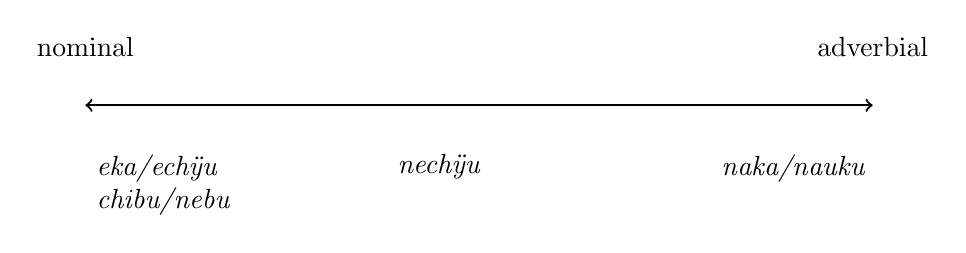
\begin{tikzpicture}
\draw [thick] [<->]  (0,0) -- (10,0);
\node[align=left, above] at (0.0, .5){nominal};%
\node[align=right, above] at (10.0, .5){adverbial};%

\node[align=left, below] at (1.0,-.5)%
    {\textit{eka/echÿu}\\
    \textit{chibu/nebu}};
\node[align=left, below] at (4.5,-.5)%
    {\textit{nechÿu}};
\node[align=left, below] at (9.0,-.5)%
    {\textit{naka/nauku}};
\end{tikzpicture}
\caption{Continuum from more nominal to more adverbial demonstratives}
\label{fig:ContinuumDEMs}
\end{figure}

A few more examples with \textit{nechÿu} follow to illustrate the exophoric use of the demonstrative. In (\getref{ex:demC-1}) and (\getref{ex:demC-5}), it refers to something that is close to the speaker but not within the current interactional space. 

In (\getref{ex:demC-1}), \textit{nechÿu} occurs with the locative-marked NP \textit{nuinekÿyae chubiu bia} ‘at the door of the church’. With this utterance, Miguel described the location of a wooden figure in relation to some other wooden toys that I had placed on my notebook. It is thus a location I had control over, but Miguel did not, thus it was not in his engagement area.\footnote{The engagement area is “the place which is, at moment \textit{t}, the conceived site of a person’s currently dominant manual and attentional engagement” \citep[89]{Enfield2003}.}

\ea\label{ex:demC-1}
\begingl
\glpreamble ja, kaku nechÿu nuinekÿyae chubiu bia\\
\gla ja kaku nechÿu nuinekÿ-yae chÿ-ubiu bia\\
\glb \textsc{afm} exist \textsc{dem}c door-\textsc{loc} 3-house God\\
\glft ‘yes, it is at the door of the church there’
\endgl
\trailingcitation{[mox-e110914l-1.076]}
\xe

In (\getref{ex:demC-5}), Juana tells me about her plans to put a cool box she had just bought in the corridor of her house to sell chicha. We were sitting in the yard, behind the house, the corridor was close to both of us, but not within our (shared) engagement area.

\ea\label{ex:demC-5}
\begingl
\glpreamble nÿsachu netuka nechÿu kureruyae\\
\gla nÿ-sachu nÿ-etuka nechÿu kureru-yae\\
\glb 1\textsc{sg}-want 1\textsc{sg}-put.\textsc{irr} \textsc{dem}c corridor-\textsc{loc}\\
\glft ‘I want to put it in the corridor over there’
\endgl
\trailingcitation{[jxx-e110923l-2.111]}
\xe

The following examples show the anaphoric use of \textit{nechÿu}, i.e. its use to refer back to an antecedent that has either been mentioned by the same speaker or by another person. In (\getref{ex:demC-6}), \textit{nechÿu} refers to the school, \textit{xhikuera}. The sentence comes from Juan C. talking with Miguel about their past and the history of the villages. They had just talked about how much San Miguelito de la Cruz had grown in the preceding decades.

\ea\label{ex:demC-6}
\begingl
\glpreamble nena tanÿma echÿu xhikuera kaku ruschÿ nechÿu, ruschÿ aula metu \\
\gla nena tanÿma echÿu xhikuera kaku ruschÿ nechÿu ruschÿ aula metu\\
\glb like now \textsc{dem}b school exist two \textsc{dem}c two room already\\
\glft ‘it is like with the school now, there are two there, two rooms already’
\endgl
\trailingcitation{[mqx-p110826l.184-186]}
\xe

A similar example is (\getref{ex:nechÿu-1}) by María S., where \textit{nechÿu} anaphorically refers to the basket, which serves as a location for clothes and some food and drink. Note that \textit{-yunu apuke} has an idiomatic meaning ‘walk, go by foot’ (lit.: ‘go ground’) as opposed to ‘go by vehicle’. 


\ea\label{ex:nechÿu-1}
\begingl
\glpreamble apuke niyunupu, apuke nupukenemÿnÿ chupaimÿnÿ nimÿu nechÿu nitapikine\\
\gla apuke ni-yunupu apuke nÿ-upukene-mÿnÿ chupai-mÿnÿ ni-mÿu nechÿu ni-tapiki-ne\\
\glb ground 1\textsc{sg}-go.to ground 1\textsc{sg}-load-\textsc{dim} basket-\textsc{dim} 1\textsc{sg}-clothes \textsc{dem}c 1\textsc{sg}-travel.supplies-\textsc{possd}\\
\glft ‘I walked, walked, with my load, a basket with my clothes in there and my travel supplies’
\endgl
\trailingcitation{[rxx-p181101l-2.036-038]}
\xe


Although \textit{nechÿu} is primarily used to encode spatial relations, the expression \textit{tukiu nechÿu} containing the \isi{source} preposition \textit{tukiu} ‘from’ is often used with a temporal meaning by Juana. This is the case in (\getref{ex:demC-3}), where there is no location in the preceding discourse that could be the referent of \textit{nechÿu}. It is rather the situation itself that is made reference to by the demonstrative.\footnote{As for the sequential \isi{connective} \textit{te}, it sometimes follows \textit{tukiu nechÿu}, but does not seem to be required. There are similar examples without \textit{te}, too.} Other speakers do not use this expression as far as I can tell from the data.

\ea\label{ex:demC-3}
\begingl
\glpreamble tukiu nechÿu te chinekupunubetuji\\
\gla tukiu nechÿu te chi-nekupu-nube-tu-ji\\
\glb from \textsc{dem}c \textsc{seq} 3-see.come-\textsc{pl}-\textsc{iam}-\textsc{rprt}\\
\glft ‘at that point they saw it coming, it is said’
\endgl
\trailingcitation{[jxx-p151016l-2.110]}
\xe


I want to conclude with (\getref{ex:demC-2}), which has the adverb \textit{nauku} ‘there’, the oblique topic pronoun \textit{nebu} and the demonstrative \textit{nechÿu} ‘\textsc{dem}c’. The adverb \textit{nauku} is used to introduce a location into the discourse. In the following clause this location is referred to by the oblique topic pronoun \textit{nebu}, which appears in first position (see \sectref{sec:FocPron}) and once the location is topical,\is{topic} it is taken up again by the demonstrative \textit{nechÿu}. The English translation is ‘there’ in all three cases. The example comes from Juana and is about her plans to move to another part of the city of Santa Cruz, where she was living at that time to care for her grandchildren.

\ea\label{ex:demC-2}
\begingl
\glpreamble biyunupuna nauku, mÿbane la feria, nebu bisemaiku, kakutu nechÿu pero mil bolivianos tÿpi entero ubiae\\
\gla bi-yunupuna nauku mÿbane {la feria} nebu bi-semaiku kaku-tu nechÿu pero mil bolivianos tÿpi entero ubiae\\
\glb 1\textsc{pl}-go.back.\textsc{irr} there close {the fair} 3\textsc{obl.top.prn} 1\textsc{pl}-search exist-\textsc{iam} \textsc{dem}c but 1000 bolivianos \textsc{obl} whole house\\
\glft ‘we may go back there, close to the fair, there we looked for it (i.e. a house), there is one now there (offered for rent), but it is (i.e. costs) 1000 bolivianos for the whole house’
\endgl
\trailingcitation{[jxx-p120430l-1.365-369]}
\xe

\is{demonstrative!demonstrative adverb|)}\is{adverb!demonstrative adverb|)}
\is{nominal demonstrative|)}



\largerpage
\subsection{Indefinite pronouns}\label{sec:IndefinitePronouns}
\is{indefinite pronoun|(}

Paunaka uses the question words\is{question word|(} \textit{chija} ‘what, who’ and \textit{juchubu} ‘where’ as indefinite pronouns with the meaning ‘something, someone’ and ‘somewhere’ respectively, see (\getref{ex:chija-INDEF2}) and (\getref{ex:juchubu-INDEF2}).

(\getref{ex:chija-INDEF2}) comes from Juana, who told me about her personal domain to speak Paunaka in the past: the way to the field she walked together with her sister María S.\footnote{This example is also interesting for the use of the verb \textit{-eiku} ‘follow’ as a \isi{preposition} with the meaning ‘along’, see also Footnote \ref{fn:along} in \sectref{sec:SerialVerbs}, and for the verb form \textit{bichujijikÿubÿu} ‘converse walking’ in which the translocative associated motion marker \textit{-CVkÿu} merges with the middle marker \textit{-bu}, but this can be considered an exception.}

\ea\label{ex:chija-INDEF2}
\begingl
\glpreamble chija echÿu bimu cheiku chenekÿ bichujijikÿubÿu bitupubu asaneti\\
\gla chija echÿu bi-imu chÿ-eiku chenekÿ bi-chujiji-kÿu-bu bi-tupu-bu asaneti\\
\glb what \textsc{dem}b 1\textsc{pl}-see 3-along? way 1\textsc{pl}-talk-\textsc{am.conc.tr}-\textsc{mid} 1\textsc{pl}-find-\textsc{mid} field\\
\glft ‘what we saw along the way we talked about walking (until) we reached the field’
\endgl
\trailingcitation{[jxx-p120430l-1.053]}
\xe

(\getref{ex:juchubu-INDEF2}) is also from Juana. She was telling me about the journey of her grandparents back home from Moxos, where they had bought cows.

\ea\label{ex:juchubu-INDEF2}
\begingl
\glpreamble juchubu kaku eka mÿiji tinikujane baka\\
\gla juchubu kaku eka mÿiji ti-niku-jane baka\\
\glb where exist grass 3i-eat-\textsc{distr} cow\\
\glft ‘where there was grass, the cows ate’
\endgl
\trailingcitation{[jxx-p151016l-2.047]}
\xe

It is relatively common cross-linguistically to use “bare interrogatives” as indefinite pronouns, i.e. interrogative pronouns that do not carry any derivational device \citep[170, 174]{Haspelmath2001}. In this scenario, the indefinite use is always secondary to the interrogative use according to \citet[5]{Haspelmath2001}, which is why \textit{chija} and \textit{juchubu} are primarily analysed as question words throughout this work (see \sectref{sec:ContentQuestions}). I also follow \citet{Haspelmath2001} in presenting \textit{juchubu} as an indefinite \textit{pronoun} while it could also be considered an indefinite \textit{adverb}\is{adverb} in a stricter sense.

Use of the indefinite pronouns is relatively rare in Paunaka and they are usually accompanied by a relative clause\is{relative relation} to provide some additional information (see also \sectref{sec:UnmarkedRC} and Footnote \ref{fn:chija} in that section), thus the construction structurally resembles a content question including a question word very much, a sign that use of the question words as indefinite pronouns is not fully grammaticalised.\is{grammaticalisation} However, regarding the use of \textit{chija}, a word of caution is necessary: speakers also use \textit{¿chija?} as a filler in hesitation (‘what was it?’), and it is thus not always clear which function the word has in a specific clause.\is{question word|)} This is the case in (\getref{ex:chija-INDEF1}), which I elicited from María S. in order to speak about Juana, who was making her house in Concepción at that time. Although \textit{chija} could well be an indefinite pronoun here semantically, intonation sets it apart from the rest of the sentence and it is preceded by a false start so it is probably rather to be analysed as a filler here:

\newpage
\ea\label{ex:chija-INDEF1}
\begingl
\glpreamble tisemaiku ti- ¿chija? tisuachi chubiupai\\
\gla ti-semaiku ti- chija ti-isua-chi chÿ-ubiupai\\
\glb 3i-search 3i- what 3i-weed.\textsc{irr}-3 3-plot\\
\glft ‘she is looking for ¿what was it? someone to weed her plot’
\endgl
\trailingcitation{[rxx-e120511l.047]}
\xe

In the other examples I give here \textit{chija} is not set apart from the rest of the sentence by intonation, pauses or false starts, thus I am fairly confident that we are dealing with the indefinite pronoun rather than with any other use of the word. There may be more examples of the indefinite use that I have mistakenly taken to represent the use as filler.

(\getref{ex:chija-INDEF3}) includes the negative particle \textit{kuina}. It is taken from María S.’s story about the two hunters who meet the devil in the woods. One man feeds the devil with the meat they hunted, but the devil does not fill up, thus finally, the man has to admit:

\ea\label{ex:chija-INDEF3}
\begingl
\glpreamble “kuinabutu chija nenikapi”\\
\gla kuina-bu-tu chija nÿ-nika-pi\\
\glb \textsc{neg}-\textsc{dsc} what 1\textsc{sg}-feed.\textsc{irr}-2\textsc{sg}\\
\glft ‘“there isn’t anything left that I could give you to eat”’
\endgl
\trailingcitation{[rxx-n120511l-2.45-46]}
\xe


The next example also contains \textit{kuina} and comes from the recordings made by Riester. Juan Ch. talks about his life in Retiro. 
%-kine = emphatic here!

\ea\label{ex:RCchija2}
\begingl
\glpreamble kuina chija baejumikine, micha bubiu nakaja\\
\gla kuina chija bi-a-ejumi-kene micha bi-ub-i-u naka-ja\\
\glb \textsc{neg} what 1\textsc{pl}-\textsc{irr}-remember-\textsc{emph}2 good 1\textsc{pl}-be-\textsc{subord}-\textsc{real} here-\textsc{emph}1\\
\glft ‘there is nothing to think about (i.e. complain about?), our living here is good’
\endgl
\trailingcitation{[nxx-p630101g-1.175]}
\xe

It is possible that \textit{chija} needs to be accompanied obligatorily by further material to be made more precise, this would explain why Juana adds \textit{echÿu} in the following example. She is making a statement here about me getting my stuff ready to travel back to Germany.

\newpage

\ea\label{ex:chija-INDEF4}
\begingl
\glpreamble komoraubinatu [...] masa arbiraubina chija echÿu\\
\gla komorau-bi-ina-tu masa arbirau-bi-ina chija echÿu\\
\glb accomodate-2\textsc{sg}-\textsc{irr.nv}-\textsc{iam} lest forget-2\textsc{sg}-\textsc{irr.nv} what \textsc{dem}b\\
\glft ‘you have to arrange (your stuff) now lest you forget something’
\endgl
\trailingcitation{[jxx-p120515l-2.276-278]}
\xe

%indirect question: ¿chijakena tububuichu eka ubiae?, kuina bichupa chija tanaubanechÿ eka ubiae, rxx-e201231f.38

In contrast, \textit{juchubu} ‘where’ can stand on its own in indefinite use, although this is rare. An example of its free use is (\getref{ex:juchubu-INDEF1}) from Juana talking about a house they want to pay with a credit.

\ea\label{ex:juchubu-INDEF1}
\begingl
\glpreamble i kue biyunatu juchubu tipuabinube tÿmuepupunuku\\
\gla i kue bi-yuna-tu juchubu ti-pua-bi-nube tÿmue-pupunuku\\
\glb and if 1\textsc{pl}-go.\textsc{irr}-\textsc{iam} where 3i-give.\textsc{irr}-1\textsc{pl}-\textsc{pl} money-\textsc{reg}\\
\glft ‘and if we go somewhere else, they give us the money back’
\endgl
\trailingcitation{[jxx-p120430l-1.388]}
\xe

Usually, however, \textit{juchubu} is also accompanied by a relative clause to specify the nature of the indefinite place as in (\getref{ex:RCwhere2}), where María S. tells Swintha about how tortoises lay their eggs.

\ea\label{ex:RCwhere2}
\begingl
\glpreamble juchubu tisachu tisukupunuka, naukuku tisekumÿnÿ epenue, tisukuka nechÿu, depue tiyunuka\\
\gla juchubu ti-sachu ti-suku-punuka nauku-uku ti-seku-mÿnÿ epenue ti-suku-uka nechÿu depue ti-yunuka\\
\glb where 3i-want 3i-lay.egg-\textsc{reg.irr} there-\textsc{add} 3i-dig.hole-\textsc{dim} hole 3i-lay.egg-\textsc{add.irr} \textsc{dem}c afterwards 3i-go.on.\textsc{irr}\\
\glft ‘where it (the tortoise) wants to lay eggs again, there it also digs a little hole to lay eggs again there, then it will go on’
\endgl
\trailingcitation{[rxx-e121128s-1.090]}
\xe

Just like in questions, \textit{juchubu} can be followed by a \isi{deranked verb} as in (\getref{ex:go-search-field-1}), elicited from Miguel.

\ea\label{ex:go-search-field-1}
\begingl
\glpreamble ukuine niyunu nisemaikupa juchubu nanaia nisaneina\\
\gla ukuine ni-yunu ni-semaiku-pa juchubu nÿ-ana-i-a ni-sane-ina\\
\glb yesterday 1\textsc{sg}-go 1\textsc{sg}-search-\textsc{dloc.irr} where 1\textsc{sg}-make-\textsc{subord}-\textsc{irr} 1\textsc{sg}-field-\textsc{irr.nv}\\
\glft ‘yesterday I went to look for somewhere to make my future field’
\endgl
\trailingcitation{[mxx-e160811sd.152]}
\xe % -> also in chapter adverbial clauses!

It is unclear at the moment which conditions favour the use of a \isi{deranked verb}, this must remain a question for further research for the time being.

\is{indefinite pronoun|)}
\is{pronoun|)}

%i tikechunubetu: eyuna n- esamaikupa juchubu ubiuyae, mxx-p110825l.051-052

%bi- bisemaiku otra juchubu bitibuia, mqx-p110826l.016

%temporal: sí aa kuina naichunabane juchubu u tu tijaibane kapunu piesta, sí, aa, antes no sabía qué día vino una fiesta, rxx-p181101l-2.013 -> indirect question?

The following section deals with adjectives, numerals, and quantifiers.



%!TEX root = 3-P_Masterdokument.tex
%!TEX encoding = UTF-8 Unicode

\section{Adjectives, numerals and quantifiers}\label{sec:AdjectivesNumerals}\is{adjective|(}

In this section, adjectives, numerals and quantifiers are described. The latter two are often subsumed under the former, but they differ from adjectives in some ways. 

There are only very few adjectives, since most property concepts are expressed by stative verbs\is{stative verb} (\sectref{sec:StativeVerbs}). Thus adjectives constitute a minor category in Paunaka. They express value, dimension, colour and shape. They are seldom used attributively in Paunaka, most of the time they occur as predicates. They are easily distinguished from verbs, since subject indexes do not precede the stem.\is{person marking|(} Indexes following the stem do not show up very frequently either, but this may be directly connected to adjectives having primarily third person referents. Occurrence of third person markers that follow the stem is very restricted in general (see \sectref{sec:3Marking}). The only adjective taking person markers from time to time is \textit{micha} ‘good’ and the adjectives derived from it. The person marker follows the adjective in this case, which is just what we expect in \isi{non-verbal predication}, see \sectref{sec:NonVerbalPredication}.\is{person marking|)} 

\textit{Micha} and its derivations are also easily distinguishable from nouns:\is{noun|(} when negated,\is{negation} a verbal form\is{verb} of the word occurs, which makes \textit{micha} suspicious of having been derived from a \isi{stative verb} originally.\footnote{Interestingly, \citet[313]{Michael2008} reports that in Nanti adjectives derived from verbs tend to occur in positive attributional clauses, while the corresponding verbs tend to occur in the negative counterparts.} 

As for other adjectives, a possibility to distinguish them from nouns is their behaviour when combining with classifiers\is{classifier|(} (see \sectref{sec:Classifiers}). If an adjective combines with a classifier, this classifier expresses a property (mostly shape) of the referent and thus it provides additional information about the referent. Nouns can also combine with classifiers, but the process resembles compounding and the product of the process is a new noun denoting a new referent. Adjectives are thus much more flexible in combining with a classifier than nouns, and they share this flexibility with the subgroup of descriptive stative verbs\is{stative verb} that can also take classifiers (\sectref{sec:StativeVerbs_CLF}). There are words, however, which are ambiguous as to whether they are nouns\is{noun|)} or should rather be analysed as adjectives.\is{classifier|)}

Numerals\is{numeral|(} are often defined as a subclass of adjectives, but there are features that distinguish them from adjectives in general. This is probably due to different functions of adjectives and numerals: “Whereas an adjective indicates a property of a noun, a numeral is not a property of the object itself but of a set of objects, often a nonce-property” \citep[770]{Greenberg2000}. In Paunaka, the most important difference is that numerals often occur attributively, while adjectives can in general occur attributively, but do not do so very frequently. Nonetheless, numerals can also be used as predicates. The only numeral of presumably Paunaka origin is \textit{chÿnachÿ} ‘one’, all numbers higher than ‘one’ have been borrowed\is{borrowing} from Spanish with different degrees of integration into Paunaka. The word for ‘other’, \textit{punachÿ} is very similar to \textit{chÿnachÿ} in the way it is composed. It is thus also treated in the section about numerals.\is{numeral|)} Both words probably contain the general \isi{classifier} \textit{-na}, which is also found on the adjectives \textit{(mu)temena} ‘big’ and \textit{kana} ‘this size’.

Quantifiers\is{quantifier} are also described in this chapter, although they were priorly analysed as adverbs because they do not frequently modify nouns, but are more often used predicatively or adverbially. However, adjectives do not often occur as nominal modifiers\is{modification} either. Semantically, quantifiers come close to numerals,\is{numeral} since both provide information about a quantity. The most frequently used quantifiers are loans\is{borrowing} from Bésiro.

In the NP,\is{noun phrase} both quantifiers\is{quantifier} and numerals\is{numeral} can only precede the noun,\is{word order} while adjectives can also follow it, although the latter case could possibly be described as a kind of \isi{modification} by a relative clause (see \sectref{sec:NP}).

\sectref{sec:Adjectives} describes adjectives in more detail, \sectref{sec:Numerals} is about numerals and the word for ‘other’ and \sectref{sec:QuantifyingAdverbs} discusses the quantifiers found in Paunaka.

\subsection{Adjectives}\label{sec:Adjectives}

There are only a few adjectives in Paunaka, thus \sectref{sec:ADJInventory} is dedicated to describing the ones that occur, while \sectref{sec:UsesADJ} examines the different usages of adjectives as predicates, attributes, adverbs, and secondary predicates.


\subsubsection{Inventory}\label{sec:ADJInventory}

The most important adjectives are \textit{micha} ‘good’, some derivations of \textit{micha}, \textit{(mu)te\-mena} ‘big’ and the \isi{demonstrative adjective} \textit{kana} ‘this size’.

The most frequent among them is \textit{micha} ‘good’. One example with it is (\getref{ex:micha-1}), which is a statement by Miguel after having looked at a puzzle game that shows a story about a boy and his squirrel.\footnote{Note that the subordinating suffix \textit{-i} creates morphologically semi-nominal words, there is no subordination involved in this example, see also \sectref{sec:AdverbialModification}.}

\ea\label{ex:micha-1}
\begingl
\glpreamble michayu chÿnÿnÿikiu eka aitubuchepÿimÿnÿ\\
\gla micha-yu chÿ-nÿnÿik-i-u eka aitubuchepÿi-mÿnÿ\\
\glb good-\textsc{ints} 3-live-\textsc{subord}-\textsc{real} \textsc{dem}a boy-\textsc{dim}\\
\glft ‘the life of the little boy is very good’
\endgl
\trailingcitation{[mdx-c120416ls.191]}
\xe

\textit{Micha} usually does not take a person marker,\is{person marking|(} with one exception: when meeting another person, people use a greeting formula including \textit{micha} and a second person index. Literally, this is a question\is{polar question} about the condition of the other. The formulaic answer is without a person marker; see (\getref{ex:ADJ-micha-1}), which is a little lecture of this convention (in Spanish) that Juana gave to Swintha.

\ea\label{ex:ADJ-micha-1}
\begingl
\glpreamble yo primero “¿michabi?” y usted me contesta “micha”\\
\gla {yo primero} micha-bi {y usted me contesta} micha\\
\glb {I first} good-2\textsc{sg} {and you me answer} good\\
\glft ‘me first “¿michabi?” (= are you doing fine?) and you answer “micha” (= fine)’
\endgl
\trailingcitation{[jxx-n101013s-1.080-083]}
\xe
\is{person marking|)}

A number of other adjectives have been derived\is{derivation|(} from \textit{micha}; these are \textit{michana} ‘nice’, which probably includes the general \isi{classifier}, a further derivation \textit{michanabÿke} ‘beautiful, pretty, handsome’ used in reference to people, which additionally takes the noun \textit{-bÿke} ‘face’,\is{incorporation} \textit{michaniki} ‘delicious’, which probably includes the verb stem\is{verbal stem} \textit{-nik(u)} ‘eat’, and \textit{michamue} ‘of sunny weather, sky without clouds’, which presumably includes the same sequence \textit{-mu} that is also found in \textit{anÿmu} ‘sky’ (as opposed to \textit{anÿke} ‘up, above’). The proposed composition of these derived adjectives is found in (\getref{ex:michana-1}) to (\getref{ex:michamue-1}), interlinear glosses of these words are usually not given in this detail in the remainder of this work.

In (\getref{ex:michana-1}), Juana talks about the house of an acquaintance in Austria.

\ea\label{ex:michana-1}
\begingl
\glpreamble michana ubiae puru teka\\
\gla micha-na ubiae puru teka\\
\glb good-\textsc{clf:}general house mere brick\\
\glft ‘the house is nice, (it has) mere bricks’
\endgl
\trailingcitation{[jxx-p110923l-2.146]}
\xe

In (\getref{ex:pretty-1}), María S. corrects my use of \textit{michana} in reference to a baby.

\ea\label{ex:pretty-1}
\begingl
\glpreamble michanabÿke\\
\gla micha-na-bÿke\\
\glb good-\textsc{clf:}general-face\\
\glft ‘she is pretty’
\endgl
\trailingcitation{[rxx-e120511l.327]}
\xe

(\getref{ex:ADJ-Pred-2}) is a statement by María S. about the fish Juana is talking about.\footnote{As for the last \textit{-i} of the word, this might be an obsolete \isi{passive} suffix. There are two hints that point at that. First of all, \isi{Mojeño Trinitario} possibly has a passive suffix in the same position on the verb ‘be delicious’ (Rose 2021, p.c.), and second, I have found one verb form in the corpus that seems to include a suffix \textit{-i} to express a \isi{passive} or at least non-agentive reading: \textit{tisamitu} (\textit{ti-sam-i-tu} 3i-hear-?-\textsc{iam}) ‘one hears (it)’ (Span. \textit{se escucha}). A final vowel /i/ of unknown origin also occurs on the stative verb stem \textit{-ÿnai} ‘be tall’, where \textit{ÿ} is the root ‘long’ and \textit{na} the general \isi{classifier}, see §\ref{sec:StativeVerbs_long}, and on the non-decomposable stem \textit{-sÿei} ‘be cold’. Note also that the adjective \textit{micha} seems to have a verbal origin, see discussion below.}

\ea\label{ex:ADJ-Pred-2}
\begingl
\glpreamble ja, michaniki\\
\gla ja micha-nik-i\\
\glb \textsc{afm} good-eat-?\\
\glft ‘yes, it is delicious’
\endgl
\trailingcitation{[jrx-c151001lsf-11.010]}
\xe

(\getref{ex:michamue-1}) was elicited from Juana.

\ea\label{ex:michamue-1}
\begingl
\glpreamble michamue\\
\gla micha-mu-e\\
\glb good-\textsc{clf:}sky?-?\\
\glft ‘the weather (lit.: sky) is nice’
\endgl
\trailingcitation{[jcx-e090727s.127]}
\xe
\is{derivation|)}

A verbal form is preferred\is{verb|(} when these concepts are negated,\is{negation} see (\getref{ex:ADJ-micha-IRR-1}) and (\getref{ex:michana-2}). Since there are no lexical antonyms, this happens relatively frequently. I would suggest that \textit{micha} originated as a \isi{stative verb} in the first place, but in positive statements, person markers were lost at some point, which then led to a hybrid behaviour of the form.

In (\getref{ex:ADJ-micha-IRR-1}), Juana talks about her mother.

\ea\label{ex:ADJ-micha-IRR-1}
\begingl
\glpreamble i tanÿma kuina tamicha chiyuikia mimi\\
\gla i tanÿma kuina ti-a-micha chi-yuik-i-a mimi\\
\glb and now \textsc{neg} 3i-\textsc{irr}-good 3-walk-\textsc{subord}-\textsc{irr} mum\\
\glft ‘and by that time my mother couldn’t walk well (lit.: her walking was not good) anymore’
\endgl
\trailingcitation{[jxx-p120430l-2.499]}
\xe

(\getref{ex:michana-2}) is about the school building in Santa Rita, which was in a miserable state. A new building was thus constructed.

\ea\label{ex:michana-2}
\begingl 
\glpreamble kuina tamichana echÿu, tikebupu echÿu\\
\gla kuina ti-a-michana echÿu ti-kebu-pu echÿu\\ 
\glb \textsc{neg} 3i-\textsc{irr}-nice \textsc{dem}b 3i-rain-\textsc{dloc} \textsc{dem}b\\ 
\glft ‘it wasn’t good, it dripped in’
\trailingcitation{[mxx-p110825l.089]}
\xe
\is{verb|)}

I have also found one example in which \textit{michanabÿke} takes a first person index preceding the stem in a positive sentence, another proof for the semi-verbal behaviour of these adjectives. In this example, (\getref{ex:pretty-2}), Juana cites the water spirit whom their grandparents met on their way back home from Moxos, where they had bought some cows. The water spirit wanted to lure away Juana’s grandfather from his wife by appearing to him at night and telling him his wife was ugly and she was beautiful. It is not clear to me why Juana used the reportive \textit{-ji} on the connective \textit{chijikiu} ‘however’, since I believe this word belongs to the quoted speech.

\ea\label{ex:pretty-2}
\begingl
\glpreamble “chÿjikiuji bien nimichanabÿke”, dice\\
\gla chÿjikiu-ji bien ni-michanabÿke dice\\
\glb however-\textsc{rprt} well 1\textsc{sg}-beautiful she.says\\
\glft ‘“however, I am very beautiful”‘ she says
\endgl
\trailingcitation{[jxx-p151016l-2.190]}
\xe

On the other hand, I have also found one non-verbal form of \textit{micha} with irrealis RS in the corpus, which is presented in (\getref{ex:ADJ-micha-IRR-2}). There are a few more examples with derived forms taking the non-verbal irrealis marker, like the one in (\getref{ex:goodweather-1}).

(\getref{ex:ADJ-micha-IRR-2}) was produced by María S. and directed to me to say farewell.

\ea\label{ex:ADJ-micha-IRR-2}
\begingl
\glpreamble ¡michaina pibÿbÿkupunia!\\
\gla micha-ina pi-bÿbÿkupun-i-a\\
\glb good-\textsc{irr.nv} 2\textsc{sg}-fly.back-\textsc{subord}-\textsc{irr}\\
\glft ‘may your flight back be good!’
\endgl
\trailingcitation{[rxx-e120511l.204]}
\xe

(\getref{ex:goodweather-1}) comes from Juana. There had been heavy rainfalls and the road where she lived was very muddy, but the forecast had announced that rain would stop for a while. Note that Juana incorrectly uses the incompletive marker \textit{-kuÿ} here instead of the discontinuous marker \textit{-bu}, but she corrected herself in the utterance that immediately followed.

\ea\label{ex:goodweather-1}
\begingl
\glpreamble michamuenatu te tajaitu kuinakuÿ tikeba\\
\gla michamue-ina-tu te tajaitu kuina-kuÿ ti-keba\\
\glb of.good.weather-\textsc{irr.nv}-\textsc{iam} \textsc{seq} tomorrow \textsc{neg}-\textsc{incmp} 3i-rain.\textsc{irr}\\
\glft ‘the weather will be nice now, tomorrow it won’t rain anymore’
\endgl
\trailingcitation{[jxx-p120515l-2.269]}
\xe

In summary, \textit{micha} and its derivations have a verbal\is{verb} and a non-verbal form. Choice is sensitive to \isi{reality status}, with \isi{realis} triggering a non-verbal and \isi{irrealis} a verbal realisation. However, the correlation is not perfect, there are a few counter-examples in the corpus.

A second relatively frequent adjective is \textit{temena}/\textit{mutemena} ‘big’. Both forms can be used interchangeably without any difference in meaning.\footnote{The first syllable \textit{mu} of the longer form \textit{mutemena} could appear to be related to the non-productive \isi{privative} marker. However, this would imply that some kind of negation is involved in the meaning of \textit{mutemena}. This is not the case: \textit{temena} and \textit{mutemena} have exactly the same meaning. The two Paunaka words containing the \isi{privative} marker are discussed in Footnote \ref{fn:privative} of \sectref{sec:Negation}.} Juana clearly prefers \textit{temena}, Miguel \textit{mutemena} and María S. seems to use both equally frequently. The last syllable \textit{na} probably goes back to the general \isi{classifier} \textit{-na} (see \sectref{sec:Classifiers}), it detaches when another classifier is added (see below).

(\getref{ex:temena-1}) is an example of the form \textit{mutemena} used by María S. in making jokes with Swintha. The other examples in this section all include the shorter form \textit{temena}.

\ea\label{ex:temena-1}
\begingl
\glpreamble aja, mutemena pichubatÿi\\
\gla aja, mutemena pi-chubatÿi\\
\glb \textsc{afm} big 2\textsc{sg}-buttocks\\
\glft ‘yes, your butt is big’
\endgl
\trailingcitation{[rxx-e121128s-4x.107]}
\xe

When the collective\is{collective|(} marker is attached to the adjective (as well as to other adjectives and verbs that end in \textit{na}), the last syllable is usually repeated. It could be the case that repetition intensifies the collective meaning, but this would not explain why it occurs with the general \isi{classifier} only, not with any other one.\footnote{There are a few cases of repetition on nouns taking the collective marker, though, see \sectref{sec:RDPL_Nouns}.} Thus repetition does not seem to indicate anything in this case (which is why it is just glossed as ‘\textsc{rep}’, i.e. ‘repetition’, here), it just comes automatically with the collective marker, as in (\getref{ex:ADJ-big-1}), where María S. talks about ripe fruits that are falling from the trees. 

\ea\label{ex:ADJ-big-1}
\begingl
\glpreamble tebakaupujanetu temenanajitu\\
\gla ti-ebakaupu-jane-tu temena-na-ji-tu\\
\glb 3i-fall.down-\textsc{distr} big-\textsc{rep}-\textsc{col}-\textsc{iam}\\
\glft ‘they (fruits) are falling down, they are big now’
\endgl
\trailingcitation{[rxx-e121128s-3.07]}
\xe
\is{collective|)}

\textit{(Mu)temena} can take classifiers\is{classifier} or combine with body-part terms\is{incorporation} and in this case \textit{-na} is dropped. (\getref{ex:ADJ-big-2}) contains a classifier and (\getref{ex:ADJ-big-3}) an inalienably possessed plant part. Both were elicited from Juana.

\ea\label{ex:ADJ-big-2}
\begingl
\glpreamble temekiji anibÿ\\
\gla teme-ki-ji anibÿ\\
\glb big-\textsc{clf:}spherical-\textsc{col} mosquito\\
\glft ‘the mosquitos are big’
\endgl
\trailingcitation{[jxx-e150925l-1.187]}
\xe

\ea\label{ex:ADJ-big-3}
\begingl
\glpreamble temepuneji\\
\gla teme-pune-ji\\
\glb big-leaf-\textsc{col}\\
\glft ‘big leaves’
\endgl
\trailingcitation{[jxx-e081025s-1.183]}
\xe

 \textit{Kana}\is{demonstrative adjective|(} ‘this size’ is a demonstrative adjective that is always accompanied by a gesture showing the size. One example is (\getref{ex:big-whip}), which comes from Miguel, who was speaking about the whip of his teacher back in the old days when he went to school in \isi{Altavista}.
 
 \ea\label{ex:big-whip}
\begingl
\glpreamble kaku echÿu asotera chija bitÿpi echÿu, kana echÿu, chimusuji eka baka\\
\gla kaku echÿu asotera chi-ija bi-tÿpi echÿu kana echÿu chi-musuji eka baka\\
\glb exist \textsc{dem}b whip 3-name 1\textsc{pl}-\textsc{obl} \textsc{dem}b this.size \textsc{dem}b 3-skin \textsc{dem}a cow\\
\glft ‘he had what we call an \textit{azotera} (= whip), it was of this size (showing with hands), made from cowhide’
\endgl
\trailingcitation{[mxx-p181027l-1.056-057]}
\xe
 
As is the case with \textit{(mu)temena}, the last syllable of \textit{kana} is repeated when a \isi{collective} marker is added, see (\getref{ex:ADJ-kana-1}) from Juana, where she speaks about some shells she needs for polishing a clay pot.

\ea\label{ex:ADJ-kana-1}
\begingl
\glpreamble kananaji micha sipÿ\\
\gla kana-na-ji micha sipÿ\\
\glb this.size-\textsc{rep}-\textsc{col} good shell\\
\glft ‘very big like this, the shells’
\endgl
\trailingcitation{[jmx-d110918ls-1.105]}
\xe\is{demonstrative adjective|)}

Apart from the adjectives presented up to here, there are a few more words that express qualities, and it is sometimes hard to decide whether they are nouns or adjectives. Consider the expressions of age such as \textit{chubui} ‘old man; old (male)’ and \textit{juberÿpu} ‘old woman; old (female)’ as well as \textit{sepitÿ} or \textit{chepitÿ} ‘child, offspring; small, little’. I treat \textit{chubui} and \textit{juberÿpu} as nouns in this grammar, and \textit{sepitÿ}/\textit{chepitÿ} as noun or adjective, depending on the context. I admit there is ambiguity in the decisions I made. There are simply no good criteria to arrive at a clear decision. Like adjectives, \textit{chubui}, \textit{juberÿpu} and \textit{sepitÿ}/\textit{chepitÿ} often occur predicatively. However, they also frequently head an NP.\is{head} In addition to these criteria, \textit{sepitÿ}/\textit{chepitÿ} can also take the limitative marker \textit{-jiku} and is then often used adverbially. In reference to non-singular participants, speakers may also use \textit{sese-ji} instead of \textit{sepitÿ}, which is probably derived\is{derivation} from the same root \textit{se}. This word, however, is usually realised as \textit{sesejinube} with the fixed meaning ‘children’, while other more adjective-like uses are very rare. Some examples that point to the words for ‘small’ being adjectives are given below.

In (\getref{ex:small1-1}), Juana uses \textit{sepitÿ} to contrast small and big clay pots.

\ea\label{ex:small1-1}
\begingl
\glpreamble sepitÿ i temena\\
\gla sepitÿ i temena\\
\glb small and big\\
\glft ‘small ones and big ones’
\endgl
\trailingcitation{[jxx-d110923l-2.35]}
\xe

(\getref{ex:small1-2}) is a statement by María S. about a tortoise.

\ea\label{ex:small1-2}
\begingl
\glpreamble sepitÿmÿnÿ chikebÿke\\
\gla sepitÿ-mÿnÿ chi-kebÿke\\
\glb small-\textsc{dim} 3-eye\\
\glft ‘its eyes are small’
\endgl
\trailingcitation{[rxx-e121128s-4x.039]}
\xe

In (\getref{ex:small2-1}), María S. makes use of \textit{sese-ji-} in speaking about some fruits that still have to ripen.

\ea\label{ex:small2-1}
\begingl
\glpreamble sesejikuÿmÿnÿ nikechubi\\
\gla sese-ji-kuÿ-mÿnÿ ni-kechu-bi\\
\glb small-\textsc{col}-\textsc{incmp}-\textsc{dim} 1\textsc{sg}-say-2\textsc{sg}\\
\glft ‘they are still very small as I said to you’
\endgl
\trailingcitation{[rxx-e121126s-3.29]}
\xe

(\getref{ex:small2-2}) was elicited from Juana and comes from the same context as (\getref{ex:ADJ-big-3}) above. It seems that the general \isi{classifier} shows up on this form together with an incorporated noun.\is{incorporation|(} Due to lack of more examples with classifiers or nouns being attached to the stem, I cannot make any judgements about this being grammatical or not. It seems strange though considering that other adjectives usually drop \textit{-na} when they combine with another \isi{classifier} or noun.

\ea\label{ex:small2-2}
\begingl
\glpreamble sesepunenaji\\
\gla sese-pune-na-ji\\
\glb small-leaf-\textsc{clf:}general?-\textsc{col}\\
\glft ‘very small leaves’
\endgl
\trailingcitation{[jxx-e081025s-1.187]}
\xe
\is{incorporation|)}

Other adjectives are \textit{enui} ‘green, not ripe, raw’ and the borrowed\is{borrowing} colour terms \textit{asuru} ‘blue’ and \textit{amariyo} ‘yellow’. All of them occur extremely infrequently in the corpus and none of them takes classifiers.\is{classifier} The reason to treat them as adjectives is a purely semantic one. The terms for ‘white’ \textit{-kipÿpa} and ‘black’ \textit{-pisÿ} are stative verbs. The term for ‘red’, \textit{tisi}, is most probably a verb, too (thus its form is actually \textit{ti-(i?)si} 3i-be.red). It is shorter than other colour terms, and it never occurs with reference to a first or second person in the corpus (and attempts to elicit such forms failed). However, \isi{Mojeño Trinitario} has a cognate form \textit{-itsi}, which is clearly a verb (Rose 2021, p.c.). \textit{Kachu-} ‘big and round’, possibly related to \textit{kana} ‘this size’, occurs twice in the corpus and takes a \isi{classifier} or inalienably possessed noun,\is{incorporation} the latter is the case in (\getref{ex:biground}) which comes from Juana who produced it in elicitation with some pictures.

\ea\label{ex:biground}
\begingl
\glpreamble isijibÿ, kachujibÿ eka tarupe\\
\gla isijibÿ kachu-jibÿ eka tarupe\\
\glb flower big.round-flower \textsc{dem}a flower.sp\\
\glft ‘a flower, the \textit{taropé} (\textit{Dorstenia brasiliensis}) has a big and round blossom’
\endgl
\trailingcitation{[jcx-e090727s.027]}
\xe

\subsubsection{Usage}\label{sec:UsesADJ}

Adjectives are used predicatively\is{attributive clause|(} most of the time, which is evident from the examples given above. If there is a noun in the sentence to which the property is predicated, the adjective usually comes first, then comes the NP. (\getref{ex:ADJ-Pred-3}) and (\getref{ex:ADJ-Pred-1}) provide two examples of this. Adjectives are also often the only constituent of a clause.

In (\getref{ex:ADJ-Pred-3}), Juana speaks about a bird of prey that once stole her dog.

\ea\label{ex:ADJ-Pred-3}
\begingl
\glpreamble temena echÿu sia\\
\gla temena echÿu sia\\
\glb big \textsc{dem}b hawk.sp\\
\glft ‘the hawk is big’
\endgl
\trailingcitation{[jxx-a120516l-a.206]}%non-el.
\xe

(\getref{ex:ADJ-Pred-1}) comes from a listing of different crops by María C.

\ea\label{ex:ADJ-Pred-1}
\begingl
\glpreamble michanikiyuku echÿu papayu\\
\gla michaniki-yu-uku echÿu papayu\\
\glb delicious-\textsc{ints}-\textsc{add} \textsc{dem}b papaya\\
\glft ‘papayas are delicious, too’
\endgl
\trailingcitation{[uxx-p110825l.193]}
\xe
\is{attributive clause|)}

Adjectives are seldom used attributively\is{modification|(} in free speech. One spontaneous example with an attributive adjective is (\getref{ex:ADJ-ATTR-1}). Juana talks about the making of pasture by the people from Santa Rita in exchange for the construction of their reservoir.

\ea\label{ex:ADJ-ATTR-1}
\begingl
\glpreamble i echÿu max temenanaji yÿkÿke kapunu makina, motosierra chibu\\
\gla i echÿu max temena-na-ji yÿkÿke kapunu makina motosierra chibu\\
\glb and \textsc{dem}b more big-\textsc{rep}-\textsc{col} tree come machine chain.saw 3\textsc{top.prn}\\
\glft ‘and [for] the biggest trees, a machine came, a chain saw more precisely’
\endgl
\trailingcitation{[jxx-p120515l-2.115]}
\xe

An example including the \isi{demonstrative adjective} \textit{kana} used as an attribute is (\getref{ex:ADJ-new-ATTR-1}). It comes from a correction session with María S. She first repeats the word her brother Miguel used in telling the story about the fox and the jaguarundi: \textit{karutemÿnÿ} ‘small club’. Probably because of the Spanish origin of this word (Span. \textit{garrote} ‘club’), she adds a Paunaka expression herself that was not used by Miguel in the original utterance, and this expression consists of a noun modified by \textit{kana}.\footnote{As for the second syllable \textit{ke} in yÿkÿkekemÿnÿ, it is actually not clear whether this is the \isi{classifier} as proposed by the glosses or repetition of the previous syllable. The noun \textit{yÿkÿke} has both meanings ‘tree’ and ‘stick’ (and also ‘wood’), and it is already derived\is{derivation} with the classifier \textit{-ke} for cylindrical items from \textit{yÿkÿ} ‘fire’, although this is probably not transparent for the speakers.}

\ea\label{ex:ADJ-new-ATTR-1}
\begingl
\glpreamble chisatÿkuji karutemÿnÿ kana yÿkÿkekemÿnÿ – ¡pa! – chikupakutu\\
\gla chi-satÿku-ji karute-mÿnÿ kana yÿkÿke-ke-mÿnÿ pa chi-kupaku-tu\\
\glb 3-cut-\textsc{rprt} club-\textsc{dim} this.size tree-\textsc{clf:}cylindrical-\textsc{dim} \textsc{idph} 3-kill-\textsc{iam}\\
\glft ‘he cut a small club, a small stick of this size, it is said, and – bang! – he killed him’
\endgl
\trailingcitation{[rxx-e150220s-2]}
\xe

There are a few more examples of nouns modified by an adjective that were produced in elicitation.\is{modification|)} 

The adjective \textit{micha} ‘good’ can also be used adverbially and translates as “well”, “nicely”, “really” or “a lot” in this case. The adjective usually follows the verb it modifies, as in (\getref{ex:ADJ-Adv-1}), but it can also precede it if emphasised, which is the case in (\getref{ex:ADJ-Adv-2}).\is{word order}

(\getref{ex:ADJ-Adv-1}) comes from Juan C. speaking about frogs.

\ea\label{ex:ADJ-Adv-1}
\begingl
\glpreamble pero yuti tikusuninechu micha peÿ\\
\gla pero yuti ti-kusuninechu micha peÿ\\
\glb but night 3i-sing good frog\\
\glft ‘but at night the frogs sing a lot’
\endgl
\trailingcitation{[mqx-p110826l.617-618]}
\xe

In (\getref{ex:ADJ-Adv-2}), Juana tells me who taught her Paunaka.

\ea\label{ex:ADJ-Adv-2}
\begingl
\glpreamble nÿuse – chibu micha timesumeikunÿ\\
\gla nÿ-use chibu micha ti-mesumeiku-nÿ\\
\glb 1\textsc{sg}-grandmother 3\textsc{top.prn} good 3i-teach-1\textsc{sg}\\
\glft ‘my grandmother – she is the one who taught me well’
\endgl
\trailingcitation{[jxx-p120430l-1.050-051]}
\xe

Adjectives are also sometimes found in depictive use, i.e. as a secondary predicate \citep[cf.][]{Schultze-Berndt2004}. This is the case in (\getref{ex:ADJ-Dep-1}), in which the adjective specifies a property of the object, which is not conominated, a corn cob that was not completely roasted yet when Swintha wanted to eat it. The warning comes from María S.

\ea\label{ex:ADJ-Dep-1}
\begingl
\glpreamble ¡masaini piniku enui!, painuepÿi\\
\gla masaini pi-niku enui p-a-inuepÿi\\
\glb \textsc{adm} 2\textsc{sg}-eat green 2\textsc{sg}-\textsc{irr}-have.wind\\
\glft ‘don’t eat it raw! You will have wind’
\endgl
\trailingcitation{[rxx-e150220s-1.25]}
\xe

\subsection{Numerals and ‘other’}\label{sec:Numerals}
\is{numeral|(}

There is only one numeral of supposedly Paunaka origin, \textit{chÿnachÿ} ‘one’, exemplified in (\getref{ex:one-3}) from Miguel, who talks about his experience in school.

\ea\label{ex:one-3}
\begingl
\glpreamble pasautu chÿnachÿ anyo nÿti nÿchupupaikutu echÿu nÿtareane\\
\gla pasau-tu chÿnachÿ anyo nÿti nÿ-chupu-paiku-tu echÿu nÿ-tarea-ne\\
\glb pass-\textsc{iam} one year 1\textsc{sg.prn} 1\textsc{sg}-know-\textsc{punct}-\textsc{iam} \textsc{dem}a 1\textsc{sg}-exercise-\textsc{possd}\\
\glft ‘one year passed and I had learned my exercises’
\endgl
\trailingcitation{[mxx-p181027l-1.087]}
\xe


The numeral consists of three parts. The first part, \textit{chÿ} seems to coincide with the third person marker\is{person marking} \textit{chÿ-}. The syllable \textit{na} may well go back to the default classifier\is{classifier|(} \textit{-na} given the fact that numerals in the related Bolivian Arawakan\is{Southern Arawakan} languages obligatorily take a classifier, and they have a classifier \textit{-no} or \textit{-na}, which serves as a default classifier \citep[147--148]{Terhart2016}. However, unlike in the related languages, the classifier \textit{-na} is lexicalised\is{lexicalisation} on the numeral, i.e. it never changes, regardless of which item is counted, and no other classifier can be elicited with the numeral. The final part of the numeral \textit{chÿnachÿ} might again be a third person marker \textit{-chÿ}, but with bleached semantics. Rose (2021, p.c.) suggests that the final syllable could be related to the \isi{limitative} marker \textit{-yÿchi}. It could also be the case that we are dealing with a restrictive marker \textit{-chÿ} cognate to  Trinitario\is{Mojeño Trinitario} \textit{-chu} here (Rose 2021, p.c.). A similar form \textit{-chu}/\textit{-chÿ}/\textit{-chÿu} sometimes occurs on question words\is{question word} (see \sectref{sec:ContentQuestions}), but is otherwise not productive in Paunaka. In any case, \textit{-chÿ} is usually omitted if other markers are attached to the numeral.\is{classifier|)}

In (\getref{ex:one-1}), Juana speaks about her daughter, who had fallen and badly injured her leg.

\ea\label{ex:one-1}
\begingl
\glpreamble eka chÿnachÿ kuje kuina puero tichema\\
\gla eka chÿnachÿ kuje kuina puero ti-chema\\
\glb \textsc{dem}a one month \textsc{neg} can 3i-stand.up.\textsc{irr}\\
\glft ‘she could not stand up for one month’
\endgl
\trailingcitation{[jxx-p110923l-1.474]}
\xe

(\getref{ex:one-2}) comes from Miguel’s story about the lazybones. Instead of making a field to nurture his family, he cuts off his own limbs in the end of the story, pretending they were \textit{cusi} palm fruits.

\ea\label{ex:one-2}
\begingl
\glpreamble chisatÿkujitu chinachÿ chijabu\\
\gla chi-satÿku-ji-tu chinachÿ chi-jabu\\
\glb 3-cut-\textsc{rprt}-\textsc{iam} one 3-leg\\
\glft ‘he cut off one of his legs, it is said’
\endgl
\trailingcitation{[mox-n110920l.097]}
\xe


The numeral is sometimes used like an indefinite article,\is{definiteness} which can be assumed is due to influence of Spanish, where the numeral \textit{uno} and the indefinite article \textit{un/una} are very similar (as is the case in many languages and directly connected to the fact that the indefinite article often derives from\is{grammaticalisation} the numeral).

(\getref{ex:one-4}) is the introductory sentence of the story about the lazybones told by Miguel.

\ea\label{ex:one-4}
\begingl
\glpreamble kakubaneji chÿnachÿ jente i tipÿkubai\\
\gla kaku-bane-ji chÿnachÿ jente i ti-pÿkubai\\
\glb exist-\textsc{rem}-\textsc{rprt} one man and 3i-be.lazy\\
\glft ‘once upon a time there was a man, it is said, and he was lazy’
\endgl
\trailingcitation{[mox-n110920l.011]}
\xe

The numeral can take the \isi{limitative} marker \textit{-jiku} and in that case, the person marker \textit{-chÿ} is detached.\is{person marking}

In (\getref{ex:one-5}), María C. asks me about my children.%\footnote{Note that she uses \textit{-checha} with the meaning of ‘daughter’ like in Bésiro, while for the other speakers of Paunaka, \textit{-checha} means ‘son’ or more generally ‘offspring’ (and also ‘egg’). \citet[48]{CarvalhoRose2018} reconstruct a noun \textit{*ʧiʧa} for Proto-Mojeño with the meaning ‘child’.}


\ea\label{ex:one-5}
\begingl
\glpreamble ¿chÿnajiku pichecha?\\
\gla chÿna-jiku pi-checha\\
\glb one-\textsc{lim}1 2\textsc{sg}-son\\
\glft ‘you have only one child?’
\endgl
\trailingcitation{[uxx-p110825l.242]}
\xe

(\getref{ex:one-6}) is from the story about the fox and the jaguarundi. The fox boasts about knowing 25 jumps, the jaguarundi has to admit to know only one (which saves him in the end, while the fox is killed).

\ea\label{ex:one-6}
\begingl
\glpreamble “kuina kakuina beintisinko nikeuchi, chÿnajiku”, tikechuji\\
\gla kuina kaku-ina beintisinko ni-keuchi chÿna-jiku ti-kechu-ji\\
\glb \textsc{neg} exist-\textsc{irr.nv} twenty-five 1\textsc{sg}-\textsc{ins} one-\textsc{lim}1 3i-say-\textsc{rprt}\\
\glft ‘“I don’t have 25, only one", he said, it is said’
\endgl
\trailingcitation{[jmx-n120429ls-x5.363]}
\xe

Finally, the number occurs in an exclamation equivalent to the English ‘oh Lord!’ or ‘good Lord!’ (Spanish ‘¡aiy señor!’), as in (\getref{ex:one-7}), which comes from Miguel. 

\ea\label{ex:one-7}
\begingl
\glpreamble ¡chÿnayue!\\
\gla chÿna-yu-e\\
\glb one-\textsc{ints}-2\textsc{pl}\\
\glft ‘good Lord!’ (lit.: ‘you (\textsc{pl}) dear one’)
\endgl
\trailingcitation{[rmx-e150922l.060]}%m
\xe

All numbers higher than ‘one’ have been borrowed\is{borrowing|(} from Spanish. Some of them also attach \textit{-chÿ}. This is obligatory with \textit{ruschÿ} ‘two’, and highly usual with \textit{treschÿ} ‘three’. From ‘four’ on, it gets less likely the higher the number in general,\footnote{Interestingly, a similar observation has been made for Trinitario\is{Mojeño Trinitario} \citep[23]{Rose2020}, and it also applies to \isi{Baure}, but it is a classifier which is more unlikely to be attached to higher numerals in those languages. Note that Trinitario and \isi{Baure} both have native numerals up to ‘three’ .} however, the numeral ‘twenty’ has also been found with \textit{-chÿ} once. The number ‘two’, \textit{ruschÿ}, is phonologically integrated into Paunaka, the Spanish word is \textit{dos} and /d/ changed to /r/ and /o/ to /u/ here. Other numerals are less integrated phonologically, e.g. the \isi{consonant cluster} in \textit{treschÿ} from Spanish \textit{tres} ‘three’ is not dissolved.\is{borrowing|)} 

(\getref{ex:two-2}) is an example of the numeral ‘two’ and (\getref{ex:three-1}) an example of ‘three’. In (\getref{ex:two-2}), Juana makes a statement about her daughter.

\ea\label{ex:two-2}
\begingl
\glpreamble kaku ruschÿ chilotene nauku\\
\gla kaku ruschÿ chi-lote-ne nauku\\
\glb exist two 3-plot-\textsc{possd} there\\
\glft ‘she has two plots there’
\endgl
\trailingcitation{[jxx-p110923l-1.421]}
\xe

(\getref{ex:three-1}) is also from Juana. She tells me about the duration of her grandson’s university studies here.

\ea\label{ex:three-1}
\begingl
\glpreamble sinko anyo tiyunuku treschÿ anyo\\
\gla sinko anyo ti-yunuku treschÿ anyo\\
\glb five year 3i-go.on three year\\
\glft ‘five years (in total), he goes on for three years’
\endgl
\trailingcitation{[jxx-p110923l-1.191]}
\xe


In (\getref{ex:two-1}), Miguel uses several numerals, ‘two’ and ‘three’ are realised with \textit{-chÿ}, but ‘four’ is not. His statement provides the answer to Swintha’s question how many baking trays of rice bread he baked together with his family. Note that the last verb is irregularly used without a subject index here.

\ea\label{ex:two-1}
\begingl
\glpreamble kuatru tipurtukabu jurnuye, pero ruschÿ banaiu entonses banaukupunuku punachÿ ruschÿ o treschÿ purtukupunuku\\
\gla kuatru ti-purtuka-bu jurnu-yae pero ruschÿ bi-ana-i-u entonses bi-anau-uku-punuku punachÿ ruschÿ o treschÿ purtuku-punuku\\
\glb four 3i-put.in.\textsc{irr}-\textsc{mid} oven-\textsc{loc} but two 1\textsc{pl}-make-\textsc{subord}-\textsc{real} thus 1\textsc{pl}-make-\textsc{add}-\textsc{reg} other two or three put.in-\textsc{reg}\\
\glft ‘four can be put into the oven, but having made two, then we made another two or three and put them in again’
\endgl
\trailingcitation{[mxx-e120415ls.096-097]}
\xe


On the other hand in (\getref{ex:four-1}), Juana uses the numeral ‘four’ with \textit{-chÿ}. The sentence refers to the picture in the end of the \isi{frog story}, where the boy finds his frog again, together with a frog lady and several little frogs.

\ea\label{ex:four-1}
\begingl
\glpreamble puru peÿjane kuatrochÿ chichecha\\
\gla puru peÿ-jane kuatruchÿ chi-checha\\
\glb mere frog-\textsc{distr} four 3-son \\
\glft ‘mere frogs, it has four children’
\endgl
\trailingcitation{[jxx-a120516l-a.435]}
\xe

Some TAME markers\is{tense}\is{aspect}\is{modality}\is{evidentiality} can attach to numerals, e.g. the \isi{iamitive} marker in (\getref{ex:two-3}), where María S. tells me about her situation.

\ea\label{ex:two-3}
\begingl
\glpreamble ruschÿtu anyo kuina nakuesanebu\\
\gla ruschÿ-tu anyo kuina nÿ-a-kuesane-bu\\
\glb two-\textsc{iam} year \textsc{neg} 1\textsc{sg}-\textsc{irr}-have.field-\textsc{dsc}\\
\glft ‘it’s already two years that I don’t have a field anymore’
\endgl
\trailingcitation{[rxx-e181017l.018]}
\xe

The numerals ‘two’ and ‘three’ can also take a person marker\is{person marking|(} in reference to humans, as in (\getref{ex:three-2}), or the \isi{plural} marker, as in (\getref{ex:three-3}). In the latter case, \textit{-chÿ} of \textit{ruschÿ} and \textit{treschÿ}, sometimes together with the final /s/ of the stem, weakens into [ʃ], [​ʂ​] or [​ʐ​], represented orthographically\is{orthography} as <xh> and <x> in the examples, and \textit{-chÿ} may then be attached if the numeral has third person reference. Thus in this case, the person marker \textit{-chÿ} seems to be involved. This is usually bound to the numeral being used predicatively, with a few counter-examples, where a numeral formed in this way is used attributively.

In (\getref{ex:three-2}), Juana speaks about the Supepí sisters who are still alive.

\ea\label{ex:three-2}
\begingl
\glpreamble i nÿti, Maria, Krara, tresxhexheikubimÿnÿ tanÿma\\
\gla i nÿti Maria Krara tresxhe-xheiku-bi-mÿnÿ tanÿma\\
\glb and 1\textsc{sg.prn} María Clara three-\textsc{cont}-1\textsc{pl}-\textsc{dim} now\\
\glft ‘and me, María, Clara, we are only three now’
\endgl
\trailingcitation{[jxx-p120430l-2.352-353]}
\xe

María C. was once severely injured by black magic. In (\getref{ex:two-predi}) she states how many frogs she had in her belly.

\ea\label{ex:two-predi}
\begingl
\glpreamble rusxenubechÿ \\
\gla rusxe-nube-chÿ\\
\glb two-\textsc{pl}-3\\
\glft ‘there were two of them’
\endgl
\trailingcitation{[ump-p110815sf.312]}
\xe

If the numeral is used attributively, the \isi{plural} marker can also be attached to it, but usually follows \textit{-chÿ} in that case and no sound change is involved, as in (\getref{ex:two-5}). The plural marker is not obligatory though.

In the following example, María S. speaks about her sister Juana, referring to the time when the family still lived more remote.

\ea\label{ex:two-5}
\begingl
\glpreamble kakutu ruschÿnube chichechajimÿnÿbane\\
\gla kaku-tu ruschÿ-nube chi-checha-ji-mÿnÿ-bane\\
\glb exist-\textsc{iam} two-\textsc{pl} 3-son-\textsc{col}-\textsc{dim}-\textsc{rem}\\
\glft ‘she already had two little children by that time long ago’
\endgl
\trailingcitation{[rxx-p181101l-2.107]}
\xe

(\getref{ex:two-4}) combines two possibilities. María S. first uses the numeral ‘two’ in an equative sentence\is{equative/proper inclusion clause} juxtaposed to a demonstrative. The demonstrative has the plural marker, the numeral does not. She then repeats the numeral as the sole predicate of a clause, and since this clause still refers to humans, the plural marker is attached to the numeral and the third person marker \textit{-chÿ} follows.\is{person marking|)} This is a statement about my children.

\ea\label{ex:two-4}
\begingl
\glpreamble ruschÿkena ekanube, rusxhunubechÿ\\
\gla ruschÿ-kena eka-nube rusxhu-nube-chÿ\\
\glb two-\textsc{uncert} \textsc{dem}a-\textsc{pl} two-\textsc{pl}-3\\
\glft ‘they are probably two, they are two’
\endgl
\trailingcitation{[rmx-e150922l.078]}
\xe

(\getref{ex:five-1}) is the only example with a numeral higher than ‘three’ that I have found taking a plural marker. It is the number ‘five’ used attributively, nonetheless, the plural marker comes first and then comes \textit{-chÿ} and finally an irrealis marker. The sentence comes from Miguel’s story about the cowherd who is enchanted by the spirit of the hill. The spirit first takes away the cows and hides them in his hill, but in the end of the story the cows are brought to a village for the people there to eat. 

\ea\label{ex:five-1}
\begingl 
\glpreamble “kapununubeina sinkonubechina jentenube ayaraunubeina bitÿpi eka bumia eka bakajane”\\
\gla kapunu-nube-ina sinko-nube-chi-ina jente-nube ayarau-nube-ina bi-tÿpi eka bi-um-i-a eka baka-jane\\ 
\glb come-\textsc{pl}-\textsc{irr.nv} five-\textsc{pl}-3-\textsc{irr.nv} man-\textsc{pl} help-\textsc{pl}-\textsc{irr.nv} 1\textsc{pl}-\textsc{obl} \textsc{dem}a 1\textsc{pl}-take-\textsc{subord}-\textsc{irr} \textsc{dem}a cow-\textsc{distr}\\ 
\glft ‘“... may five men come to help us take the cows”’
\trailingcitation{[mxx-n151017l-1.78]}
\xe

Dates and times of the day are realised with Spanish numerals without attachment of \textit{-chÿ}. As for times of the day, the numeral is usually accompanied by the Spanish feminine article \textit{la(s)} and regarding ‘one o’clock’ and ‘two o‘clock’, the numerals \textit{una} and \textit{dos} are used rather than the Paunaka ones as in (\getref{ex:num-time-1}) and (\getref{ex:num-time-2}).

(\getref{ex:num-time-1}) is the answer of María S. to my question whether she had been to Concepción. Note that the verb does not carry the middle marker here, which is unusual, especially since there is no overt goal.

\ea\label{ex:num-time-1}
\begingl
\glpreamble hm, nitupunu la una\\
\gla hm ni-tupunu {la una}\\
\glb \textsc{afm} 1\textsc{sg}-reach {at one o’clock}\\
\glft ‘hm, I arrived at one o’clock’
\endgl
\trailingcitation{[rxx-e120511l.002]}
\xe

(\getref{ex:num-time-2}) comes from Juana telling me about the last things her brother did before he suddenly and unexpectedly died.

\newpage

\ea\label{ex:num-time-2}
\begingl
\glpreamble titupunubuji nauku las doskena\\
\gla ti-tupunubu-ji nauku {las dos}-kena\\
\glb 3i-arrive-\textsc{rprt} there {at two o’clock}-\textsc{uncert}\\
\glft ‘he arrived there at two o’clock maybe, it is said’
\endgl
\trailingcitation{[jxx-p120430l-2.404]}
\xe

The noun \textit{tose} ‘noon’ has possibly been borrowed\is{borrowing} from \isi{Bésiro}, although it presumably originates from the Spanish numeral \textit{doce} ‘twelve’. \textit{Tose} is exclusively used with reference to the midday, if the number is meant, speakers use \textit{dose},\footnote{Surprisingly, in Trinitario\is{Mojeño Trinitario} it is the other way round: \textit{te las doce} means ‘at noon’ and \textit{ntose} is used for counting (Rose 2021, p.c.).} compare (\getref{ex:twelve-1}) with the noun and (\getref{ex:twelve-2}) with the numeral.

(\getref{ex:twelve-1}) is a question by Clara directed to Swintha and me. We had been to Santa Rita that same day before visiting her and María C.

\ea\label{ex:twelve-1}
\begingl
\glpreamble ¿tose etupupunubu o kupeitu?\\
\gla tose e-tupupunu-bu o kupei-tu\\
\glb noon 2\textsc{pl}-arrive.back-\textsc{mid} or afternoon-\textsc{iam}\\
\glft ‘did you arrive back (from Santa Rita) at noon or in the afternoon?’
\endgl
\trailingcitation{[cux-c120414ls-2.332]}
\xe

(\getref{ex:twelve-2}) comes from Miguel telling the history of Santa Rita, which was founded after people were let free from forced labour in \isi{Altavista}.

\ea\label{ex:twelve-2}
\begingl 
\glpreamble kapunutu kuineini taitaini pero kapununube dose familia\\
\gla kapunu-tu kuineini taita-ini pero kapunu-nube dose familia\\ 
\glb come-\textsc{iam} deceased dad-\textsc{dec} but come-\textsc{pl} twelve family\\ 
\glft ‘my late father had come (here), but twelve families came (altogether)’
\trailingcitation{[mxx-p110825l.056]}
\xe

The word for ‘other’ is \textit{punachÿ}. It resembles the numeral \textit{chÿnachÿ} in the way it is composed. The first syllable \textit{pu} is possibly related to the Proto-Arawakan numeral \textit{*pa-} ‘one’, which has developed into an impersonal \isi{pronoun} in some \isi{Arawakan languages} \citep[85]{Aikhenvald1999}.\is{numeral|)} Sometimes, Juana preposes a /u/ yielding \textit{upunachÿ}, but this is more frequent in the derived forms (see below).\footnote{The preposed /u/ is expected by the \isi{stress} pattern (see \sectref{sec:Stress}), and it also relates Paunaka to \isi{Mojeño Trinitario}, where the cognate form \textit{(‘)po-na} sometimes occurs with an initial glottal stop that corresponds to a syncopated vowel (Rose 2021, p.c.).}

\textit{Punachÿ} can be used as a modifier\is{modification} as in (\getref{ex:other-2}) or head an NP as in (\getref{ex:other-3}).\is{head} 

In (\getref{ex:other-2}), Juana tells me about her plans to move to another house in Santa Cruz together with the family of her daughter.

\ea\label{ex:other-2}
\begingl
\glpreamble repente bisemaika punachÿ kuarto nauku\\
\gla repente bi-semaika punachÿ kuarto nauku\\
\glb maybe 1\textsc{pl}-search.\textsc{irr} other room there\\
\glft ‘maybe we want to look for another room (i.e. house with one more room) there’
\endgl
\trailingcitation{[jxx-p120430l-1.355]}
\xe

%\ea\label{ex:other-1}
%\begingl
%\glpreamble i punachÿ kaku Espanya\\
%\gla i punachÿ kaku Espanya\\
%\glb and other exist Spain \\
%\glft ‘and there is another one in Spain’\\
%\endgl
%\trailingcitation{[jxx-e120516l-1.028]}
%\xe


Interestingly, in (\getref{ex:other-3}) María S. uses \textit{punachÿ} twice to contrast two men, where English (and also Spanish) would use the numeral ‘one’ in contrast with ‘other’. There are more examples in the corpus that point into a similar direction, but none is as clear as this one. It comes from the story about the two men who meet the devil in the woods. One of them interacts with the devil and is finally eaten, the other hides away on a tree and can escape in the end.

\ea\label{ex:other-3}
\begingl
\glpreamble echÿu punachÿ tipunu anÿke, mhm, i echÿu punachÿ kuina tipunaji ...\\
\gla echÿu punachÿ ti-punu anÿke mhm i echÿu punachÿ kuina ti-puna-ji\\
\glb \textsc{dem}a other 3i-go.up up \textsc{intj} and \textsc{dem}a other \textsc{neg} 3i-go.up.\textsc{irr}-\textsc{rprt}\\
\glft ‘one of them climbed up, mhm, and the other one didn’t climb up, it is said...’
\endgl
\trailingcitation{[rxx-n120511l-2.32-35]}
\xe


Like numerals, \textit{punachÿ} can attach some markers. The final \textit{-chÿ} is sometimes detached, but this happens relatively infrequently. Consider  (\getref{ex:other-4}) and (\getref{ex:other-5}), which come from Miguel and María S. respectively and were produced one after the other. In (\getref{ex:other-4}), the irrealis and the uncertainty marker are attached to the full form \textit{punachÿ}, in (\getref{ex:other-5}), the final \textit{-chÿ} is detached and replaced by the irrealis marker. Both sentences refer to my announced return to Bolivia. Note that in local Spanish, people use ‘other’ in combination with a temporal noun to refer to the next day, week, month or year, although this is not very precise and can sometimes also refer to the time unit following the next one.

\ea\label{ex:other-4}
\begingl
\glpreamble punachinakena anyo tibÿsÿupunuka\\
\gla punachÿ-ina-kena anyo ti-bÿsÿu-punuka\\
\glb other-\textsc{irr.nv}-\textsc{uncert} year 3i-come-\textsc{reg.irr}\\
\glft ‘maybe next year she will come back’
\endgl
\trailingcitation{[mrx-c120509l.125]}
\xe

\ea\label{ex:other-5}
\begingl
\glpreamble ¿puneina anyo pibÿsÿupunuka?\\
\gla puna-ina anyo pi-bÿsÿu-punuka\\
\glb other-\textsc{irr.nv} year 2\textsc{sg}-come-\textsc{reg.irr}\\
\glft ‘you will come back next year?’
\endgl
\trailingcitation{[mrx-c120509l.126]}
\xe


Unlike \textit{chÿnachÿ}, \textit{punachÿ} can detach the supposed \isi{classifier} \textit{-na} in three cases. First of all, it can combine with the \isi{verbal root} \textit{-jai} ‘be light, day’ followed by a syllable \textit{-ne}, which is probably the possessed marker (see \sectref{sec:Alienables}), yielding \textit{(u)pujaine} ‘the other day’. Second, it can also combine with the relational noun \textit{-akene} ‘non-visible side’ as \textit{(u)puakene} ‘other side’.\footnote{When combining with a person marker, this noun is also sometimes pronounced \textit{-ekene}, see \sectref{sec:Locative}.} Whether the initial /u/ occurs on both words seems to be bound to the rhythm of the whole sentence. Third, the \isi{distributive} marker is attached directly to the root, in this case the \isi{plural} marker usually follows the distributive (except for one example in the corpus), thus the form is \textit{pujanenube} ‘the others’. It is often used to refer to ‘all the others’, but not exclusively. While \textit{(u)puakene} is often found with a third person marker following it, \textit{(u)pujaine} and \textit{pujanenube} never take a third person marker. One example of each derived form is given below.\is{derivation|(}

In (\getref{ex:other-6}), Juana talks about one of her daughters building a house.

\ea\label{ex:other-6}
\begingl
\glpreamble ja’a puakenechÿ tanaunube chubiunubeina\\
\gla ja’a pu-akene-chÿ ti-anau-nube chÿ-ubiu-nube-ina\\
\glb \textsc{afm} other-non.vis.side-3 3i-make-\textsc{pl} 3-house-\textsc{pl}-\textsc{irr.nv}\\
\glft ‘yes, on the other side (of the street) they are making their future house’
\endgl
\trailingcitation{[jxx-p110923l-2.154]}
\xe

(\getref{ex:other-7}) comes from María S. telling me about the former times, or more precisely, the food her mother cooked in former times.

\ea\label{ex:other-7}
\begingl
\glpreamble chÿnachÿ tijai tiyÿtikapumÿnÿ arusuji pujaine pujukekepupunukutu tiniku\\
\gla chÿnachÿ tijai ti-yÿtikapu-mÿnÿ arusu-ji pu-jai-ne pujukeke-pupunuku-tu ti-niku\\
\glb one day 3i-cook.\textsc{irr}-\textsc{dim} rice-\textsc{clf:}soft.mass other-day-\textsc{possd} patasca-\textsc{reg}-\textsc{iam} 3i-eat\\
\glft ‘one day she would cook a rice stew, the other day she ate \textit{patasca} again’
\endgl
\trailingcitation{[rxx-p181101l-2.250]}
\xe

Finally in (\getref{ex:other-8}) from the same recording as the previous example, María S. explained me why she did not have friends when she was a child. She lived with her family a little remote, while other families already settled in the place where the village of Santa Rita is located until now.

\ea\label{ex:other-8}
\begingl
\glpreamble chijikiu pujanenube naka chubiunube\\
\gla chijikiu pu-jane-nube naka chÿ-ubiu-nube\\
\glb however other-\textsc{distr}-\textsc{pl} here 3-house-\textsc{pl}\\
\glft ‘in contrast, all the others had their houses here’
\endgl
\trailingcitation{[rxx-p181101l-2.119]}
\xe
\is{derivation|)}

\subsection{Quantifiers}\label{sec:QuantifyingAdverbs}
\is{quantifier|(}

Quantifiers provide information about the quantity of something. They can modify nouns, but only marginally. More often, they are used as heads of NPs,\is{head} as predicates (see also \sectref{sec:NP}) or they modify a \isi{verb}. \tabref{table:QuantifyingAdverbs} provides an overview of the quantifiers found in the corpus.

\begin{table}[htbp]
\caption[Quantifiers]{Quantifiers}

\begin{tabular}{lll}
\lsptoprule
Quantifier & Translation & Comment\cr
\midrule
\textit{chama} & much, many, a lot & loan from Bésiro \cr
\textit{pariki} & many, much, a lot  & \cr
\textit{pario} & some, something, to some degree & loan from Bésiro \cr
\textit{pasayu} & much, a lot & \cr
\textit{musume} & many & \cr
\textit{tumuyubu} & all & lexicalised from verb \cr
\lspbottomrule
\end{tabular}

\label{table:QuantifyingAdverbs}
\end{table}

The quantifier \textit{pario} has been borrowed\is{borrowing|(} from \isi{Bésiro} \citep[cf.][333]{FussRiester1986}, and \textit{pariki} seems to be related to it. However, I do not know whether the latter one is also used in Bésiro or has been derived from the former in Paunaka. While \textit{pario} encodes that something holds to some degree as in (\getref{ex:pario-ex}), \textit{pariki} tells us that something holds to a high degree as in (\getref{ex:pariki-ex}).\is{borrowing|)} Synonym with the latter is \textit{musume} as in (\getref{ex:musume-ex}), which is also sometimes given as \textit{musube}.

(\getref{ex:pario-ex}) comes from María C. who echoes a prior statement by Clara about her son. This kind of echoing is frequently used in conversation as a back-channelling device. 

\ea\label{ex:pario-ex}
\begingl
\glpreamble tichupumÿnÿ pario paunaka\\
\gla ti-chupu-mÿnÿ pario paunaka\\
\glb 3i-know-\textsc{dim} some Paunaka\\
\glft ‘he knows some Paunaka’
\endgl
\trailingcitation{[cux-c120414ls-2.269]}
\xe

In (\getref{ex:pariki-ex}), Juana makes a statement about the water reservoir of Santa Rita.

\ea\label{ex:pariki-ex}
\begingl
\glpreamble pariki jimu nechÿu\\
\gla pariki jimu nechÿu\\
\glb many fish \textsc{dem}c\\
\glft ‘there is a lot of fish’
\endgl
\trailingcitation{[jxx-p120515l-2.135]}
\xe

In (\getref{ex:musume-ex}), Juana talks about the viciousness of the \textit{karay} who, realising that the speakers’ grandparents had bought many cows, made plans to usurp them.

\ea\label{ex:musume-ex}
\begingl
\glpreamble chimunube musume, te tiyunukunubetu chibejiukunubetu chipeu baka\\
\gla chi-imu-nube musume te ti-yunuku-nube-tu chi-bejiuku-nube-tu chi-peu baka\\
\glb 3-see-\textsc{pl} many \textsc{seq} 3i-go.on-\textsc{pl}-\textsc{iam} 3-take.away-\textsc{pl}-\textsc{iam} 3-animal cow\\
\glft ‘they saw that there were many (cows), so they went to take away their cows’
\endgl
\trailingcitation{[jxx-e150925l-1.258]}%non-el.
\xe

While both \textit{pariki} and \textit{musume} are predominantly used for countable items, \textit{chama} is used with non-countable things, e.g. water. Compare (\getref{ex:chama-1}) to (\getref{ex:pariki-ex}) above. 

(\getref{ex:chama-1}) is also about a water reservoir, but this time about the one in \isi{Altavista}. The statement comes from Clara.

\ea\label{ex:chama-1}
\begingl
\glpreamble chama ÿne nechÿu\\
\gla chama ÿne nechÿu\\
\glb much water \textsc{dem}c\\
\glft ‘there is a lot of water there’
\endgl
\trailingcitation{[cux-c120414ls-1.207]}
\xe


María C. produced (\getref{ex:chama-verb}) when we were making fun about being drunk (resulting from Swintha asking Clara for the word for ‘be drunk’.)

\ea\label{ex:chama-verb}
\begingl
\glpreamble chama teukena\\
\gla chama ti-eu-kena\\
\glb much 3i-drink-\textsc{uncert}\\
\glft ‘maybe she has drunk a lot’
\endgl
\trailingcitation{[cux-c120414ls-1.056]}
\xe

However, \textit{pariki} is sometimes also found in connection with non-countable and \textit{chama} with countable things.

An alternative to \textit{chama} is \textit{pasayu} ‘much, a lot’, but it is used less often and majorly by María S. (\getref{ex:pasayu-n}), however, is an example that stems from the recordings made by Riester in the 1960s. Juan Ch. talks about the amount of work he is forced to do, in this case weeding in the peanut plantation:

\ea\label{ex:pasayu-n}
\begingl
\glpreamble ... pasayu chikeuchi bipatrunenube\\
\gla pasayu chi-keuchi bi-patrun-ne-nube\\
\glb much 3-\textsc{inst} 1\textsc{pl}-patrón-\textsc{possd}-\textsc{pl}\\
\glft ‘it is a lot because of our \textit{patrones}’
\endgl
\trailingcitation{[nxx-p630101g-2.26]}
\xe


(\getref{ex:pario-verb}) is an example of an adverbial use of a quantifier. It comes from Miguel telling José the \isi{frog story}. It refers to the picture on which the boy sees the beehive.

\ea\label{ex:pario-verb}
\begingl
\glpreamble i naka tiyuyuikutu pario eka aitubuchepÿimÿnÿ\\
\gla i naka ti-iyuyuiku-tu pario eka aitubuchepÿi-mÿnÿ\\
\glb and here 3i-cry-\textsc{iam} some \textsc{dem}a boy-\textsc{dim}\\
\glft ‘and here the little boy is crying a bit’
\endgl
\trailingcitation{[mox-a110920l-2.067]}
\xe


The quantifier \textit{tumuyubu} looks like a lexicalised\is{lexicalisation} middle verb\is{middle voice} (see \sectref{sec:Middle_voice}). It can possibly be decomposed as \textit{ti-umu-bu-yu} (3i-take-\textsc{mid}-\textsc{ints}) ‘much is taken’. Its meaning is ‘all, everything’. One example is (\getref{ex:tumuyubu-2}). A very small part of Juana’s speech is omitted from this example, since she only confirms a side question of me and then goes on with her utterance. She lists all the things a couple from Germany had brought to Concepción in order to sell them in their shop.

\ea\label{ex:tumuyubu-2}
\begingl
\glpreamble tupununube mÿiji (...) i tumuyubu tÿmuepa yubuti eka kuicha, tumuyubu\\
\gla ti-upunu-nube mÿiji i tumuyubu tÿmuepa yubuti eka kuicha tumuyubu\\
\glb 3i-bring-\textsc{pl} grass and all knife axe \textsc{dem}a spade all\\
\glft ‘they brought grass (seeds) (...) and everything, knifes, axes, spades, everything’
\endgl
\trailingcitation{[jxx-p120515l-2.036-039]}
\xe

If the referent is human, the \isi{plural} marker can be added to the quantifier. One example of this is given in (\getref{ex:tumuyubu-1}), where \textit{tumuyubunube} ‘all of them’ is the subject of the non-verbal motion predicate. This example also comes from Juana and refers to the people of Santa Rita who had all planned to come to Concepción to see the appearance of Evo Morales in the multi-purpose hall.

\ea\label{ex:tumuyubu-1}
\begingl
\glpreamble tumuyubunube kapununubeina\\
\gla tumuyubu-nube kapunu-nube-ina\\
\glb all-\textsc{pl} come-\textsc{pl}-\textsc{irr.nv}\\
\glft ‘they will all come’
\endgl
\trailingcitation{[jxx-p150920l.079]}
\xe

\is{quantifier|)}
\is{adjective|)}

%chaama = mucho: Sans 2013:63
% Bésiro poco = chímyantai, pequeño: chimyámantai, algunos: eanákiatai ubutúriki, harto: sɨrɨmána (Sans 2010:151)

This was the last example of this section, the following one deals with adverbs.




















%!TEX root = 3-P_Masterdokument.tex
%!TEX encoding = UTF-8 Unicode

\section{Adverbs}\label{sec:Adverbs}\is{adverb|(}

Adverbs typically form a large heterogeneous class. They have been described as “a ‘catch-all’ category” that lumps together “[a]ny word with semantic content (i.e., other than grammatical particles) that is not clearly a noun, a verb, or an adjective” \citep[69]{Payne1997}. Adverbs typically modify, but unlike adjectives, they do not primarily modify nouns but verbs, adjectives,\is{adjective} other adverbs, nouns and full clauses \citep[715]{Evans2000}.

The adverbs of Paunaka are not marked for person\is{person marking} or for number and they do not take the locative marker \textit{-yae}, either. They cannot occur as arguments of a verb and they are never modified\is{modification} by a nominal demonstrative. This definition excludes some locative words which are often used adverbially, but are rather analysed as nouns due to their ability to occur with the locative marker or as an argument of a verb. %and also some temporal nouns and verbs: \textit{yuti} ‘night’, \textit{tijai} ‘day’.

\hspace*{-1.3pt}Adverbs can be subdivided into subclasses depending on their semantics. There are spatial (\sectref{sec:LocativeAdverbs}), temporal and aspectual (\sectref{sec:TemporalAspectualAdverbs}), and modal (\sectref{sec:ModalAdverbs}) adverbs. The different subclasses of adverbs can take different modal, temporal, aspectual and/or other markers.



\subsection{Locative adverbs}\label{sec:LocativeAdverbs}
\is{locative|(}

\largerpage
Locative adverbs provide clues about the spatial setting of an event. They definitely comprise the demonstrative adverbs\is{adverb!demonstrative adverb|(}\is{demonstrative!demonstrative adverb|(} \textit{naka} ‘here’ and \textit{nauku} ‘there’, i.e. not here, (far) away, see (\ref{ex:here-there}). What exactly is perceived as “here” varies, as it does in other languages, and largely depends on the situational “engagement area” of a speaker, i.e. the space that she is currently focused on by paying attention to this space and acting in it \citep[cf.][89]{Enfield2003}.\footnote{It should be mentioned here that the use of \textit{naka} ‘here’ and \textit{nauku} ‘there’ sometimes runs counter to my intuition. It remains to be analysed how Paunaka speakers conceptualise their here-sphere. See \citet[251--257]{Admiraal2016} for an analysis of “here” in closely related Baure.}  In addition, there is another demonstrative, \textit{nechÿu} glossed as ‘\textsc{dem}c’, with the approximate meaning of ‘in that place, there’, i.e. in an identifiable place of mostly medial distance. \textit{Nechÿu} has nominal and adverbial properties. This has been described in more detail in \sectref{sec:DemPron}. The locative adverbs are given in \tabref{table:SpatialWords}.

\begin{table}
\caption{Locative adverbs}

\begin{tabular}{lll}
\lsptoprule
Adverb & Translation & Comment\cr
\midrule
\textit{naka} &  here & demonstrative adverb \cr
\textit{nauku} &  there (distal) & demonstrative adverb \cr
\textit{nechÿu} & there (medial) & nominal/adverbial demonstrative\cr
\lspbottomrule
 \end{tabular}

\label{table:SpatialWords}
\end{table}

%\textit{anÿke} & up & noun or adverb\cr
%\textit{apuke} & down, on the ground & noun or adverb\cr
%\textit{mÿbane(jiku)} & close, near & adverb derived from a stative verb\cr
%\textit{pÿkÿjÿe} & in the middle & noun or adverb\cr

In (\ref{ex:here-there}), Juana uses two demonstrative adverbs. She speaks about a relocation within the city of Santa Cruz after her grandson finished his premilitary service.

\ea\label{ex:here-there}
\begingl
\glpreamble tukiu nauku tanÿma bibÿsÿu naka\\
\gla tukiu nauku tanÿma bi-bÿsÿu naka\\
\glb from there now 1\textsc{pl}-come here\\
\glft ‘from there we came here now’
\endgl
\trailingcitation{[jxx-p110923l-1.182]}
\xe


The demonstrative adverbs (including \textit{nechÿu}) can be used on their own or be accompanied by a noun phrase that specifies the exact location.

In (\ref{ex:naka-1}), the location meant by \textit{naka} is shown by a gesture, thus no NP co-occurs. \textit{Naka} refers to the belly of the María C. in this case, where a sorcerer had introduced a frog.

\ea\label{ex:naka-1}
\begingl
\glpreamble ani naka peÿ\\
\gla ani naka peÿ\\
\glb look here frog\\
\glft ‘look, here [I had] a frog’
\endgl
\trailingcitation{[ump-p110815sf.300]}
\xe

In (\ref{ex:naka-2}) María C. specifies what she means by \textit{naka} with a prepositional phrase. She had moved from Santa Rita to Concepción that year and was now living next to Clara. Note that she drops the second person singular person marker on the verb, which is typical for her speech, but not necessarily accepted by the other speakers.


\ea\label{ex:naka-2}
\begingl
\glpreamble simukunÿ naka tÿpi eka nipiji\\
\gla simuku-nÿ naka tÿpi eka ni-piji\\
\glb find-1\textsc{sg} here \textsc{obl} \textsc{dem}a 1\textsc{sg}-sibling\\
\glft ‘you have found me here at my sister’s’
\endgl
\trailingcitation{[cux-120410ls.007]}
\xe

In (\ref{ex:nauku-1}), the distal adverb \textit{nauku} is used. The exact location that it refers to is unknown, at least to me, the addressee. Specific location is not important in this context, the utterance is rather about Clara being away from her house, which is included in the here-location of that situation – the yard of María C.’s house next to Clara’s house.

\ea\label{ex:nauku-1}
\begingl
\glpreamble tiyunu nauku, mhm, trabaku\\
\gla ti-yunu nauku mhm trabaku\\
\glb 3i-go there \textsc{intj} work\\
\glft ‘she went there, mhm, in order to work’
\endgl
\trailingcitation{[uxx-e120427l.089]}
\xe

In (\ref{ex:nauku-2}) on the other hand, the exact location of \textit{nauku} is of importance, since this sentence is about origin. Thus an NP\is{noun phrase} is used together with the adverb. \textit{Nauku} conveys the additional information that the exact location, Santa Rita, is in a not-here sphere for María C., not in her engagement area anymore, since she had moved to Concepción to live with her son’s family after her husband had died.


\ea\label{ex:nauku-2}
\begingl
\glpreamble nÿti tukiu nauku Santa Rita\\
\gla nÿti tukiu nauku {Santa Rita}\\
\glb 1\textsc{sg.prn} from there {Santa Rita}\\
\glft ‘I am from Santa Rita there’
\endgl
\trailingcitation{[cux-120410ls.010]}
\xe


(\ref{ex:nechÿu-2}) provides an example of \textit{nechÿu}, more examples can be found in \sectref{sec:DemPron}. It comes from a narrative by Miguel, the exact location to which \textit{nechÿu} refers directly follows; a type of basket which can be carried. Into this basket, the limbs of the main character of the story are stored, which he had just cut off and given to his son pretending they were racemes of \textit{cusi} palm fruit.

\ea\label{ex:nechÿu-2}
\begingl
\glpreamble bueno, chikamureikuji echÿu chinachÿ chijabu punachÿ chijabu nechÿu sÿkikÿyae\\
\gla bueno chi-kamureiku-ji echÿu chinachÿ chi-jabu punachÿ chi-jabu nechÿu sÿki-kÿ-yae\\
\glb well 3-accommodate-\textsc{rprt} \textsc{dem}b one 3-leg other 3-leg \textsc{dem}c basket-\textsc{clf}:bounded-\textsc{loc}\\
\glft ‘well, he accommodated his one leg and his other leg there in the basket, it is said’
\endgl
\trailingcitation{[mox-n110920l.110]}
\xe
\is{adverb!demonstrative adverb|)}\is{demonstrative!demonstrative adverb|)}


As for the rest of the spatial words,\is{word class|(} it is not clear to me at the moment whether they should rather be classified as adverbs or nouns.\is{noun|(} The antonyms \textit{nujekÿ} ‘inside’ and \textit{nekupai} ‘outside, yard’ are mainly used adverbially. But both also occur with the locative marker occasionally, which might be a hint that they are nouns rather than adverbs. On the other hand, none of them is modified by nominal demonstratives in the corpus, which might be a hint that they are adverbs rather than nouns. The same holds for the two words that describe a horizontal axis, \textit{anÿke} ‘up, above’ and \textit{apuke} ‘ground, down’, the latter one occasionally takes a locative marker when it refers to the ground, but it has not been found on \textit{anÿke} in the corpus.\is{noun|)}

Thus if we consider only (\ref{ex:apuke-3}), \textit{apuke} could well be an adverb. It describes the direction of gaze of Juana’s daughter, when she was sitting in an airplane and only saw water below her.

\ea\label{ex:apuke-3}
\begingl
\glpreamble timumuku apuke\\
\gla ti-imumuku apuke\\
\glb 3i-look ground\\
\glft ‘she looked down’
\endgl
\trailingcitation{[jxx-p110923l-1.412]}
\xe

In (\ref{ex:apuke-1}), however, which comes from Miguel, \textit{apuke} takes a locative marker. It is used as a noun that denotes the ground as our known world, which is contrasted in the story with the world inside the hill, where the spirit lives.

\ea\label{ex:apuke-1}
\begingl
\glpreamble tibÿchÿupupunukuji naka apukeyae\\
\gla ti-bÿchÿu-pupunuku-ji naka apuke-yae\\
\glb 3i-leave-\textsc{reg}-\textsc{rprt} here ground-\textsc{loc}\\
\glft ‘he left to the ground here again, it is said (i.e. this world after having been inside the hill with the spirit)’
\endgl
\trailingcitation{[mxx-n151017l-1.58]}
\xe

\textit{Apuke} can even be the object of a verb, as in (\ref{ex:apuke-2}), which comes from Juana and is from her account about her grandparents’ journey to Moxos. On their way back home, they are surprised by heavy rainfalls and have to pass an arroyo that has filled with water.

\ea\label{ex:apuke-2}
\begingl
\glpreamble kuinaji chitupa apuke\\
\gla kuina-ji chi-tupa apuke\\
\glb \textsc{neg}-\textsc{rprt} 3-find.\textsc{irr} ground\\
\glft ‘she didn’t reach the ground (of the river with her feet), it is said’
\endgl
\trailingcitation{[jxx-p151016l-2.144]}
\xe

%\ea\label{ex:apuke-11}
%\begingl
%\glpreamble tiyupunutu pitikiri tukiu apuke\\
%\gla ti-yupunu-tu pitikiri tukiu apuke\\
%\glb 3i-come.out-\textsc{iam} cicada.sp from ground\\
%\glft ‘the cicada emerges from the ground’\\
%\endgl
%\trailingcitation{[rxx-e181021les.119]}
%\xe

%naka+ -tu, -ni, -ja{'a), -uku, -upunu, -jiku, -yÿchi, -kena, -pupunu, -mÿnÿ, -bane, kuina nakabu
%nauku + -uku, -bane, -jiku, -tu, -bÿti, -ni, -ja'a

%naka (795 hits): here, close, what is conceived as "here" varies like in English (depending on the contrast, what is perceived as not here)
%nechÿu (103 hits): something, which is easily identifiable because it has just been talked about or it is specified just after or it can be seen
%nauku (573 hits): more distant than nechÿu, including emotional/temporal/discourse distance

Thus, two kinds of overlaps concerning spatial words can be found. First, there is an overlap between nominal and adverbial function of the demonstrative adverb \textit{nechÿu}, and second, certain words with spatial semantics do not neatly fit into either of the categories of noun and adverb.
\is{word class|)}
\is{locative|)}



\subsection{Temporal and aspectual adverbs}\label{sec:TemporalAspectualAdverbs}\is{temporal/aspectual|(}

Temporal and aspectual adverbs comprise those words that provide information about the temporal setting of an event, its internal constituency or its relation to another event.

\tabref{table:TemporalAdverbs} lists the temporal and aspectual adverbs. In addition, there are a few more words referring to times of the day that are probably rather nouns than adverbs, although they are used adverbially most of the time. Among them are \textit{mane} ‘morning’, \textit{tose} ‘noon, midday’, \textit{kupei} ‘afternoon’ (also used with the meaning ‘late’ as its equivalent \textit{tarde} in Spanish), \textit{yuti} ‘night’. \textit{Mane}, \textit{kupei} and \textit{yuti} can be modified by a nominal demonstrative, but this happens rarely. \textit{Tose} occurs with the locative marker \textit{-yae} once in the corpus. The word for ‘day‘, \textit{tijai}, is a stative verb, and so are the words derived\is{derivation} from it, e.g. \textit{tijaikenekÿu} ‘dawn’, \textit{tajaitu} ‘tomorrow’ or \textit{tajaibÿti} with the idiomatic meaning ‘see you tomorrow/another day'.

\begin{table}
\caption{Temporal and aspectual adverbs}

\begin{tabularx}{\textwidth}{lQ}
\lsptoprule
Adverb & Translation \cr
\midrule
\textit{abane} & finally \cr
\textit{janeka} & never \cr
\textit{maneiku} & soon \cr
\textit{metu} & already \cr
\textit{nÿmayu} & just\cr
\textit{tanÿma} &  now  \cr
\textit{(u)chuine} & just now, recently, a few moments to hours ago, same day \cr
\textit{ukuine} & yesterday, a few days ago \cr
\textit{(u)kuinebu} & some day in the intermediate past, a few days, weeks or months ago\cr
\textit{upunuku} & again \cr
\lspbottomrule
 \end{tabularx}

\label{table:TemporalAdverbs}
\end{table}

%\textit{uchu} &  some day in an uncertain future \cr

%tanÿma: 265 hits = jetzt now
%uchuine: 26 hits = gerade eben just recently, a few moments ago
% uchu: some day, uncertain future


%janeka chikurabaka = que nadie lo quebre??, jmx-d110918ls-1.078
%mqx-p110826l.556

The\is{iamitive|(} adverb \textit{metu} ‘already’ is used very frequently and probably the source for the iamitive marker \textit{-tu} (see \sectref{sec:Iamitive}). Just like the iamitive marker,\is{iamitive|)} \textit{metu} can be used both when an event is completed, (\ref{ex:ADVmetu-1}), and when it is ongoing at the moment in question, (\ref{ex:ADVmetu-2}), with or without a connotation of earliness. Thus, depending on the specific context and the aktionsart of the predicate, ‘now’ is sometimes a more appropriate translation than ‘already’. \textit{Metu} always precedes the predicate.

(\ref{ex:ADVmetu-1}) was elicited from María S. and refers to an imagined pot.

\ea\label{ex:ADVmetu-1}
\begingl
\glpreamble nimutu metu terabajikutu\\
\gla ni-imu-tu metu ti-rabajiku-tu\\
\glb 1\textsc{sg}-see-\textsc{iam} already 3i-break-\textsc{iam}\\
\glft ‘when I saw it, it was already broken’
\endgl
\trailingcitation{[rxx-e181021les.222]}
\xe

(\ref{ex:ADVmetu-2}) is a statement by Juana about herself.

\ea\label{ex:ADVmetu-2}
\begingl
\glpreamble nÿti metu juberÿpunÿtu\\
\gla nÿti metu juberÿpu-nÿ-tu\\
\glb 1\textsc{sg.prn} already old.woman-1\textsc{sg}-\textsc{iam}\\
\glft ‘I am old already/now’
\endgl
\trailingcitation{[jxx-p110923l-1.205]}
\xe

Equally frequent is \textit{tanÿma} ‘now’. This adverb might have originated from a stative verb, the initial \textit{t} being a fixed third person marker, and \textit{-nÿma} an \isi{associated motion} marker (see \sectref{sec:SubsequentMotion}). However, the word is totally lexicalised. When a morpheme is added, especially \textit{-yu}, the first syllable is usually dropped today, resulting in a form \textit{nÿmayu}. In the recordings by Riester, we find the full form \textit{tanÿmayu}. \textit{Nÿmayu} is punctual and best translated as ‘just’.

(\ref{ex:ADVnow}) is a statement by María S. which refers to me having changed the position of my chair a bit because the sun was shining on me. When I was sitting in the shade again, she said:

\ea\label{ex:ADVnow}
\begingl
\glpreamble michatu tanÿma\\
\gla micha-tu tanÿma\\
\glb good-\textsc{iam} now\\
\glft ‘now it is good’
\endgl
\trailingcitation{[rxx-e181024l.019]}
\xe

(\ref{ex:ADVjust}) comes from Juana and refers to the work the people of Santa Rita did for a lady from Germany in exchange for the construction of the reservoir.

\ea\label{ex:ADVjust}
\begingl
\glpreamble juu nÿmayu tijaipai tiyununubetu techikanube\\
\gla juu nÿmayu ti-jai-pai ti-yunu-nube-tu ti-echika-nube\\
\glb \textsc{intj} just 3i-be.light-\textsc{clf:}ground 3i-go-\textsc{pl}-\textsc{iam} 3i-fell.tree.\textsc{irr}-\textsc{pl}\\
\glft ‘oh, when it just began to dawn (lit.: there was just light on the ground), they already went to fell trees’
\endgl
\trailingcitation{[jxx-p120515l-2.179]}
\xe

The adverb \textit{(u)chuine} is used if the point in time is not considered as “now” because the event expressed by the verb is completed, but it is still perceived as something in the very recent past, as in (\ref{ex:uchuine}). The word is only used to refer to points in time of the current day.\is{past reference} It may be derived\is{derivation} from the \isi{uncertain future} marker \textit{uchu} ‘some day (perhaps, in an uncertain future)’ (see \sectref{sec:UncertainFuture}), at the same time it resembles the adverb \textit{ukuine} ‘yesterday, some day in the recent past’, which also refers to a recent past, but less recent than the current day, see (\ref{ex:ukuine}). The translation with ‘yesterday’ is not very precise, since \textit{ukuine} can also refer to the day before yesterday or another day in the recent past. However, most of the times it is used to refer to the day preceding the current day.

(\ref{ex:uchuine}) is a statement by Juana about her daughter including \textit{uchuine}.

\ea\label{ex:uchuine}
\begingl
\glpreamble uchuine chÿnachÿtu ora tichujiku tukiu nauku\\
\gla uchuine chÿnachÿ-tu ora ti-chujiku tukiu nauku\\
\glb just.now one-\textsc{iam} hour 3i-speak from there\\
\glft ‘just an hour ago she talked [with me] from there (on telephone)’
\endgl
\trailingcitation{[jxx-p120430l-1.335-336]}
\xe

(\ref{ex:ukuine}) contains \textit{ukuine} and also comes from Juana, who tells me about the source of her knowledge about her brother’s health.

\ea\label{ex:ukuine}
\begingl
\glpreamble chikuetea chijinepÿi ukuine\\
\gla chi-kuetea chi-jinepÿi ukuine\\
\glb 3-tell 3-daughter yesterday\\
\glft ‘his daughter told it [to me] yesterday (or a few days ago)’
\endgl
\trailingcitation{[jxx-e150925l-1.124]}
\xe

In addition, \textit{(u)kuinebu} refers to points in time in an intermediate past\is{past reference} which may be some days ago, but also some weeks or months ago, as in (\ref{ex:ukuinebu}), which was recorded in April and the event that Juana is referring to happened some months ago: some friends of the daughter who live in Argentina came to visit her over New Year and brought some coffee as a present.

\ea\label{ex:ukuinebu}
\begingl
\glpreamble nauku Argentina tupununube uikuinebu\\
\gla nauku Argentina ti-upunu-nube uikuinebu\\
\glb there Argentina 3i-bring-\textsc{pl} some.time.ago\\
\glft ‘they brought it  from Argentina some time ago’
\endgl
\trailingcitation{[jxx-e120430l-4.28]}
\xe


The adverbs \textit{tanÿma} and \textit{(u)chuine} can be intensified by a marker \textit{-paiku/a}, which narrows the possible time frame.\footnote{This marker also shows up on verbs,\is{verb} but very infrequently. I suppose it fulfils the same function there.} (\ref{ex:right-now}) comes from Miguel who told us a story, while we sat to eat and relax a bit on our visit to \isi{Altavista}.

\ea\label{ex:right-now}
\begingl
\glpreamble ... tiyuna paseana nenabi biti tanÿmapaiku\\
\gla ti-yuna pasea-ina nena-bi biti tanÿma-paiku\\
\glb 3i-go.\textsc{irr} stroll-\textsc{irr.nv} like-1\textsc{pl} 1\textsc{pl.prn} now-\textsc{punct}\\
\glft ‘... he will go on a jaunt like we are doing right now’
\endgl
\trailingcitation{[mxx-n120423lsf-X.15]}
\xe

%tanÿmapaiku nÿpikeika, kuinakuÿ nÿbuka = ahorita estoy atiendo, todavía no he terminado, rxx-e181022le


In (\ref{ex:chuinepaiku}), María S. asks me about my arrival in Santa Rita that day.

\ea\label{ex:chuinepaiku}
\begingl
\glpreamble ¿chuinepaiku pitupunubu?\\
\gla chuine-paiku pi-tupunubu\\
\glb just.now-\textsc{punct} 2\textsc{sg}-arrive\\
\glft ‘you have just arrived?’
\endgl
\trailingcitation{[rxx-e120511l.005]}
\xe

The adverb \textit{maneiku} ‘soon’ is probably derived\is{derivation} from \textit{mane} ‘morning’. It is used very infrequently. One example is given in (\ref{ex:maneiku}), where Juana makes a statement about my departure to Germany being close in contrast to Swintha’s, who had plans to stay a bit longer.

\ea\label{ex:maneiku}
\begingl
\glpreamble asi max temprano piyunupuna, maneiku piyuna\\
\gla asi max temprano pi-yunupuna maneiku pi-yuna\\
\glb so more early 2\textsc{sg}-go.back.\textsc{irr} soon 2\textsc{sg}-go.\textsc{irr}\\
\glft ‘so you go back earlier, you go soon’
\endgl
\trailingcitation{[jxx-p120430l-2.635]}
\xe

\textit{Janeka} ‘never’ seldom shows up in the corpus, but one example from Juana is given below. It is not clear to me why she uses realis RS here. She speaks about the pot she was going to make with the clay she had just collected.

\ea\label{ex:janeka}
\begingl
\glpreamble janeka chikurabaku\\
\gla janeka chi-kurabaku\\
\glb never 3-break\\
\glft ‘nobody ever breaks it’ (lit.: ‘never [a non-specified agent] breaks it’)
\endgl
\trailingcitation{[jmx-d110918ls-1.078]}
\xe

%semantics of janeka not totally clear (n has: ti(bi)janeka)

Finally, there is \textit{abane}, which means ‘finally’. It expresses that something that has been expected is completed after a time span that is considered (too) long, as in (\ref{ex:abane-2-2}), where Juana’s daughter finally calls her boss to accompany her to the airport and speak to the people in charge to put in a good word for her sister who had arrived to Spain without a valid visa.

\ea\label{ex:abane-2-2}
\begingl
\glpreamble abane chichujiku te tiyununubetu\\
\gla abane chi-chujiku te ti-yunu-nube-tu\\
\glb finally 3-speak \textsc{seq} 3i-go-\textsc{pl}-\textsc{iam}\\
\glft ‘finally she spoke to him and they went (to the airport)’
\endgl
\trailingcitation{[jxx-p110923l-1.351]}
\xe
\is{temporal/aspectual|)}


\subsection{Modal adverbs}\label{sec:ModalAdverbs}\is{modal|(}

Modal meanings are seldom expressed by adverbs, since most information of this kind is marked on the predicate or more rarely other constituents of the clause (see \sectref{sec:Modality_Evidentiality}). However, a few modal adverbs are used in Paunaka and they are given in \tabref{table:ModalAdverbs}. 

\begin{table}
\caption{Modal adverbs}

\begin{tabular}{lll}
\lsptoprule
Adverb & Translation & Comment\cr
\midrule
\textit{nakayenetu} & almost & proximate\cr
\textit{nakayenetÿini} & almost & avertive\cr
\textit{repente} & maybe & loan from Spanish \cr
\lspbottomrule
 \end{tabular}

\label{table:ModalAdverbs}
\end{table}


\textit{Repente} is a loan\is{borrowing} from Spanish \textit{de repente} ‘maybe’ (also ‘suddenly’, which is also another meaning of the Paunaka word, but less frequently). It is more or less synonym with the \isi{uncertainty} marker \textit{(-)kena}, which expresses uncertainty (see \sectref{sec:ModalityUncertainty}). \textit{Kena} is phonologically bound to another word most of the time, and it can also attach to \textit{repente}. \textit{Repente} has some variants \textit{pente} and \textit{depente}, but they are less frequent than \textit{repente}. (\ref{ex:repente}) offers one example of the adverb, which comes from Miguel when talking with María C. about her husband, who was ill.

\ea\label{ex:repente}
\begingl
\glpreamble pero repentekena michaupunu punachina semana\\
\gla pero repente-kena micha-upunu punachÿ-ina semana\\
\glb but maybe-\textsc{uncert} good-\textsc{reg} other-\textsc{irr} week\\
\glft ‘but maybe he has recovered (lit.: is good again) next week’
\endgl
\trailingcitation{[mux-c110810l.037]}
\xe


The\is{avertive|(} adverb \textit{nakayenetu/nakayenetÿini} ‘almost’ is complex,\is{derivation} at least as its ending is concerned. It contains either the \isi{iamitive} marker \textit{-tu} or the avertive marker \textit{-tÿini} (see \sectref{sec:Iamitive} for iamitive aspect and \sectref{sec:FRUST-Avertive} for avertive modality). As for the rest of the word, \textit{naka} could derive from the demonstrative adverb (see \sectref{sec:LocativeAdverbs} above), and \textit{yene} could relate to the \isi{deductive} marker \textit{-yenu} (\sectref{sec:Epistemic_Mod}), but this is speculative. In any way, the difference between both variants of the adverb is that \textit{nakayenetu} is proximate, i.e. the event is temporally close and realisable, while \textit{nakayenetÿini} is avertive, i.e. the event was imminent but did not occur.


(\ref{ex:almost-prox}) is one example of the proximate use of the adverb. Juana answers my question here, when they were going to eat.

\ea\label{ex:almost-prox}
\begingl
\glpreamble nakayenetu toseina binika\\
\gla nakayenetu tuse-ina bi-nika\\
\glb almost noon-\textsc{irr.nv} 1\textsc{pl}-eat.\textsc{irr}\\
\glft ‘we will eat just before noon’
\endgl
\trailingcitation{[jxx-p110923l-2.099]}
\xe

(\ref{ex:almost-2}) gives one example of the avertive version of the adverb. Juana was searching for the Paunaka name for ‘deer’, there must have been one and it must have sounded similar to \textit{yÿnÿ} ‘jabiru’ (a bird: \textit{Jabiru mycteria}).

\ea\label{ex:almost-2}
\begingl
\glpreamble nakayenetÿini chija eka nikecha yÿnÿ\\
\gla nakayenetÿini chi-ija eka ni-kecha yÿnÿ\\
\glb almost 3-name \textsc{dem}a 1\textsc{sg}-say.\textsc{irr} jabiru\\
\glft ‘I would have almost said \textit{yÿnÿ} (i.e. jabiru) is its name’
\endgl
\trailingcitation{[jxx-a120516l-a.240-241]}
\xe
\is{avertive|)}
\is{modal|)}
\is{adverb|)}



The following section describes prepositions.



%!TEX root = 3-P_Masterdokument.tex
%!TEX encoding = UTF-8 Unicode
\section{Prepositions}\label{sec:Adpositions}
\is{preposition|(}
\is{oblique|(}

There are four words that can be analysed as prepositions, they are given in \tabref{table:Adpositions}. These prepositions are used to mark constituents as obliques (see \sectref{sec:DeclClausesOBL}). They encode an instrument, a causer,\is{instrument/cause} \isi{source}, benefactive,\is{beneficiary}\footnote{In the index at the end of this book, the semantic role “benefactive” is encoded as “beneficiary”, because the term “benefactive” is reserved for a suffix that changes the valency of a verb.} aim or result\is{aim/result}, \isi{recipient} or a \isi{comitative} relation.  

\begin{table}
\caption{Prepositions}

\begin{tabularx}{\textwidth}{llQ}
\lsptoprule
Preposition & Translation & Comment \cr
\midrule
\textit{-aj(i)echubu} & with & always person-marked, least grammaticalised preposition \cr
\textit{-keuchi} & by, with & usually with person marker, but possible without\cr
\textit{tukiu} & from & never person-marked \cr
\textit{(-)tÿpi }& \textsc{obl}, for & possible with and without person marker, also used for clause-linking \cr
\lspbottomrule
\end{tabularx}

\label{table:Adpositions}
\end{table}

Typical examples for the prepositions are given in (\getfullref{ex:new23-preps.1}) to (\getfullref{ex:new23-preps.4}).

\ea\label{ex:new23-preps}
  \ea\label{ex:new23-preps.1}
\begingl
\glpreamble chajechubu nÿenu\\
\gla chÿ-ajechubu nÿ-enu\\
\glb 3-\textsc{com} 1\textsc{sg}-mother\\
\glft ‘with my mother’
\endgl
\trailingcitation{[rxx-p181101l-2.044]}
  \ex\label{ex:new23-preps.2}
\begingl
\glpreamble chikeuchi yÿkÿke\\
\gla chi-keuchi yÿkÿke\\
\glb 3-\textsc{ins} stick\\
\glft ‘with a stick’
\endgl
\trailingcitation{[jxx-p120430l-1.073]}
  \ex\label{ex:new23-preps.3}
\begingl
\glpreamble tukiu Naranjito\\
\gla tukiu Naranjito\\
\glb from Naranjito\\
\glft ‘from Naranjito’
\endgl
\trailingcitation{[mxx-p110825l.183]}
  \ex\label{ex:new23-preps.4}
\begingl
\glpreamble chitÿpi echÿu patron\\
\gla chi-tÿpi echÿu patron\\
\glb 3-\textsc{obl} \textsc{dem}b patrón\\
\glft ‘for the \textit{patrón}’
\endgl
\trailingcitation{[mxx-p110825l.025]}
\z
\xe

As illustrated by these examples, prepositions are always placed before the NP\is{noun phrase|(} they are related to. Nonetheless, not all of them necessarily occur together with an NP: if they take a first or second person marker,\is{person marking|(} no NP shows up with the preposition, and if they take a third person marker, an NP is optional. The \isi{source} preposition \textit{tukiu} is never marked for person. Consequently, it always occurs together with a noun or an adverb. The \isi{comitative} preposition \textit{-aj(i)echubu} is always marked for person. The \isi{instrument/cause} preposition \textit{-keuchi} is normally person-marked and only rarely drops a third person index. As regards \textit{(-)tÿpi}, first and second person markers are obligatory, while the third person marker usually alternates with an NP, although sometimes there is both a third person index on the preposition and an NP\is{noun phrase|)} following it, especially if the referent is human.\is{person marking|)}\is{animacy}

In addition to the prepositions presented in this section, Paunaka makes use of a few words that express specific spatial relations to a referent. This is often achieved by using adpositions in other languages, but in Paunaka these words are better analysed as relational nouns,\is{relational noun|(} since they obligatorily take the locative marker to specify that a spatial relation is expressed (see \sectref{sec:Locative}). If a noun is juxtaposed to the relational noun, it can be regarded its \isi{possessor}. The possessor noun does not take the locative marker. In contrast to relational nouns, the locative marker is never attached to the prepositions, not even to \textit{tukiu}, which is used to mark \isi{source} expressions, i.e. a spatial relation. However, the noun that \textit{tukiu} relates to can take the \is{locative marker}. This is illustrated in (\ref{ex:adp-1}) and (\ref{ex:adp-2}). In (\ref{ex:adp-1}) the locative marker is attached to the noun following the preposition and the preposition itself is unmarked. In (\ref{ex:adp-2}), the locative marker is attached to the relational noun and its \isi{possessor} is unmarked.\is{relational noun|)}

(\ref{ex:adp-1}) was produced by Miguel in talking with Juan C. about their past. 

\ea\label{ex:adp-1}
\begingl
\glpreamble ja bibÿsÿupunu tukiu Turuxhiyae sinkuenta i dos\\
\gla ja bi-bÿsÿupunu tukiu Turuxhi-yae {sinkuenta i dos}\\
\glb \textsc{afm} 1\textsc{pl}-come from Altavista-\textsc{loc} {fifty-two}\\
\glft ‘well, we came from \isi{Altavista} in 52’
\endgl
\trailingcitation{[mqx-p110826l.055]}
\xe

(\ref{ex:adp-2}) also comes from Miguel and refers to the picture in the \isi{frog story} in which the dog stands on a log (and the boy leans over that log).

\ea\label{ex:adp-2}
\begingl
\glpreamble tijipuikutuji chÿineyae echÿu yÿkÿke\\
\gla ti-jipuiku-tu-ji chÿ-ine-yae echÿu yÿkÿke\\
\glb 3i-jump-\textsc{iam}-\textsc{rprt} 3-top-\textsc{loc} \textsc{dem}b tree\\
\glft ‘it has jumped on top of the log, it is said’
\endgl
\trailingcitation{[mtx-a110906l.207]}
\xe


The degree of \isi{grammaticalisation} of the prepositions differs with the verbal origin being still recognisable in the \isi{instrument/cause} preposition \textit{-keuchi} and the \isi{comitative} \textit{-aj(i)echubu}, while the sources of the prepositions \textit{(-)tÿpi} and \textit{tukiu} are not clear. This will be explained in more detail in the sections that follow. The source preposition \textit{tukiu} is described in \sectref{sec:adp-tukiu}, the many different functions of the general oblique marker \textit{(-)tÿpi} are illustrated in \sectref{sec:adp-tÿpi}, the instrument and cause preposition \textit{-keuchi} is described in \sectref{sec:adp-keuchi}, and finally \sectref{sec:adp-ajechubu} is dedicated to the least grammaticalised adpostion, the comitative marker \textit{-aj(i)echubu}.

\subsection{The source preposition}\label{sec:adp-tukiu}
\is{source|(}

The preposition \textit{tukiu} introduces source expressions and thus occurs a lot in sentences describing motion events. It never takes a person marker.\is{person marking} 

(\ref{ex:new23adp-tukiu}) was provided by María S. and referred to a present I gave her.

\ea\label{ex:new23adp-tukiu}
\begingl
\glpreamble tukiu Alemania pupunu\\
\gla tukiu Alemania pi-upunu\\
\glb from Germany 2\textsc{sg}-bring\\
\glft ‘you brought it from Germany’
\endgl
\trailingcitation{[rxx-e120511l.016]}
\xe

The initial \textit{t} of the preposition could be a hint that it derives\is{grammaticalisation} from a \isi{verb} inflected with the third person marker \textit{ti-}, \textit{u} we also find in the defective verb \textit{-ubu} ‘be, live’.\footnote{This verb probably contains the middle marker\is{middle voice} \textit{-bu}, thus its root is \textit{u}.} The sequence \textit{kiu} resembles what we find in deranked verbs, a \isi{thematic suffix} + subordinate marking, but then again, deranked verbs rather take the third person marker \textit{chÿ-} instead of \textit{ti-} (see \sectref{sec:Subordination-i}).\footnote{Note that Rose (2021, p.c.) proposes a link to the \isi{Mojeño Trinitario} verb \textit{os’o} ‘come from, be from’. This could possibly also explain the sequence \textit{kiu}. There is no related verb in Paunaka synchronically.}

\textit{Tukiu} is usually preposed to a noun or a locative adverb \is{adverb|(}, especially \textit{naka} ‘here’ and \textit{nauku} ‘there’. Locative adverb and noun also often combine to yield a more precise source expression. If there is a noun in the source expression, it can take the \isi{locative marker} \textit{-yae}, but this is not always the case. Adverbs never take this marker.\is{adverb|)}

In (\ref{ex:adp-tukiu-1}), the toponym\is{toponym|(} noun in the source expression bears the locative marker. The example is from María C.’s account about her life. She was once very ill and went to San Pedrito crawling, where they extracted two frogs from her belly. Note that she does not use the verb for ‘crawl’ in this sentence, but resorts to a collocation with a Spanish origin, \textit{kuatrupie} from \textit{a cuatro pies} ‘on hands and knees’, which is used adverbially.

\ea\label{ex:adp-tukiu-1}
\begingl
\glpreamble kuatrupie niyunu San Pedrito tukiu Arubeituyae\\
\gla {kuatrupie} ni-yunu {San Pedrito} tukiu Arubeitu-yae\\
\glb {on.hands.and.knees} 1\textsc{sg}-go {San Pedrito} from Arubeito-\textsc{loc}\\
\glft ‘on hands and knees I went to San Pedrito from Arubeito’
\endgl
\trailingcitation{[ump-p110815sf.303]}
\xe

(\ref{ex:adp-tukiu-3}) has a source expression in which the toponym (i.e. a noun) occurs without a locative marker. It was produced by Juana while sitting at her house in Concepción. She informed me about the plans of the inhabitants of Santa Rita to participate in the public appearance of Evo Morales in Concepción in 2015.

\ea\label{ex:adp-tukiu-3}
\begingl
\glpreamble aja las ocho naka kapununubeina titupunapunube tukiu Santa Rita\\
\gla aja {las ocho} naka kapunu-nube-ina ti-tupunapu-nube tukiu {Santa Rita}\\
\glb \textsc{intj} {at eight o’clock} here come-\textsc{pl}-\textsc{irr.nv} 3i-arrive.\textsc{irr}-\textsc{pl} from {Santa Rita}\\
\glft ‘yes, at eight o’clock they will come here, they will arrive from Santa Rita’
\endgl
\trailingcitation{[jxx-p150920l.078]}
\xe
\is{toponym}

In (\ref{ex:adp-tukiu-7}), the source is expressed with the adverb \textit{nauku} ‘there’. This sentence stems from Juana. I had been waiting for her at the zoo, when she had just arrived home from elsewhere.

\ea\label{ex:adp-tukiu-7}
\begingl
\glpreamble las dies nibÿsÿu tukiu nauku, nubiuyae\\
\gla {las dies} ni-bÿsÿu tukiu nauku nÿ-ubiu-yae\\
\glb {at ten o’clock} 1\textsc{sg}-come from there 1\textsc{sg}-house-\textsc{loc}\\
\glft ‘at ten I came home from there, to my house’
\endgl
\trailingcitation{[jxx-p110923l-2.043]}
\xe

In the source expression of (\ref{ex:adp-tukiu-4}), we have both the adverb \textit{nauku} and a complex locative expression containing the relational noun \textit{-chuku} ‘side’. The sentence comes from María S., who told me about her life. The family had once lived more remote from where Santa Rita is located today. Only José remained in this remote location, the other siblings moved away. 

\ea\label{ex:adp-tukiu-4}
\begingl
\glpreamble bijechikutu tukiu nauku chukuyae Kose\\
\gla bi-jechiku-tu tukiu nauku chi-chuku-yae Kose\\
\glb 1\textsc{pl}-move-\textsc{iam} from there 3-side-\textsc{loc} José\\
\glft ‘we moved from there close to José’s’
\endgl
\trailingcitation{[rxx-p181101l-2.257]}
\xe

In (\ref{ex:new23-adp-tukiu2}), Juana combines \textit{naka} with a toponym. She compares the coffee from Argentina she received as a present to the coffee from Bolivia here.

\ea\label{ex:new23-adp-tukiu2}
\begingl
\glpreamble max michaniki eka tukiu naka Bolivia\\
\gla max michaniki eka tukiu naka Bolivia\\
\glb more delicious \textsc{dem}a from here Bolivia\\
\glft ‘the one from here, from Bolivia is better’
\endgl
\trailingcitation{[jxx-e120430l-4.37]}
\xe

The source preposition is also often used to encode sources of non-motion events. It might be the case that this is due to influence of Spanish, which would also make use of the source preposition \textit{de} to encode these cases. Two examples of this use are given below, both were produced by Juana.

In the first of these examples, the source is a source of knowledge, not of motion along a path. It comes from Juana’s account about her encounter with two old Paunaka ladies, who first did not recognise that she understood them talking in Paunaka. In (\ref{ex:adp-tukiu-5}), Juana cites what one of the ladies said to her after Juana had introduced herself to them.

\ea\label{ex:adp-tukiu-5}
\begingl
\glpreamble “ja'a nichupuikubane pia tukiu Turuxhiyae”\\
\gla ja'a ni-chupuiku-bane pi-a tukiu Turuxhi-yae\\
\glb \textsc{afm} 1\textsc{sg}-know-\textsc{rem} 2\textsc{sg}-father from Altavista-\textsc{loc} \\
\glft ‘“yes, I know your father from \isi{Altavista} in the old days”’
\endgl
\trailingcitation{[jxx-p120515l-1.134]}
\xe

(\ref{ex:adp-tukiu-6}) is from the story about the fox and the jaguar. The jaguar has already drowned in a pond at this point of the story. Some months later, approximately in August, the fox comes back to speak with the skeleton of the jaguar. The pond has fallen dry by that time.

\ea\label{ex:adp-tukiu-6}
\begingl
\glpreamble tibukubutu echÿu ÿne tukiu nechÿu kurichiyae\\
\gla ti-buku-bu-tu echÿu ÿne tukiu nechÿu kurichi-yae\\
\glb 3i-finish-\textsc{mid}-\textsc{iam} \textsc{dem}b water from \textsc{dem}c pond-\textsc{loc}\\
\glft ‘the water had vanished (lit.: finished) from the pond’
\endgl
\trailingcitation{[jmx-n120429ls-x5.283]}
\xe

\is{source|)}

The following section is dedicated to the general oblique marker \textit{(-)tÿpi}, which is the most frequent preposition.

\subsection{The oblique preposition}\label{sec:adp-tÿpi}
\is{general oblique|(}

The preposition \textit{(-)tÿpi} is the one found with the largest array of different functions and is thus simply glossed ‘\textsc{obl}’ for ‘oblique’. It is often used with constituents that have the semantic role of a benefactive,\is{beneficiary} but also with aims or results,\is{aim/result} recipients,\is{recipient} temporal expressions, and sometimes also with goals. The preposition is also used to introduce purpose clauses. In general, \textit{(-)tÿpi} can be found in most of the contexts in which the speakers would use the prepositions \textit{para} or \textit{por} (both among other things mean ‘for’), when speaking Spanish.

As for its origin, there is a stative verb \textit{-tÿpina} ‘be straight, be correct’, but the similarity to the preposition may be coincidental. If the preposition is in some way related to the verb, the semantic connection has become opaque. 

In what follows, I give examples for the many different uses of \textit{(-)tÿpi}. Among the most frequent are the expression of benefactives\is{beneficiary|(} and results or aims.\is{aim/result} To illustrate these uses, compare the following two examples, in which \textit{(-)tÿpi} is used once to mark a benefactive constituent in (\ref{ex:adp-tÿpi-2}) and once to mark a result or aim in (\ref{ex:adp-tÿpi-3}). They were both produced by Juana in an elicitation session, but (\ref{ex:adp-tÿpi-2}) was requested as a translation of a Spanish sentence and (\ref{ex:adp-tÿpi-3}) was added by Juana herself.

\ea\label{ex:adp-tÿpi-2}
\begingl
\glpreamble nupunu eka merÿ pitÿpi\\
\gla nÿ-upunu eka merÿ pi-tÿpi\\
\glb 1\textsc{sg}-bring \textsc{dem}a plantain 2\textsc{sg}-\textsc{obl}\\
\glft ‘I brought these plantains for you’
\endgl
\trailingcitation{[jxx-e191021e-2]}
\xe

\ea\label{ex:adp-tÿpi-3}
\begingl
\glpreamble bupunu echÿu merÿ tÿpi masakujina\\
\gla bi-upunu echÿu merÿ tÿpi masaku-ji-ina\\
\glb 1\textsc{pl}-bring \textsc{dem}b plantain \textsc{obl} masaco-\textsc{clf:}soft.mass-\textsc{irr.nv}\\
\glft ‘we brought these plantains for \textit{masaco} (a dish made with plantains and cheese)’
\endgl
\trailingcitation{[jxx-e191021e-2]}
\xe

An example with two benefactives introduced by \textit{(-)tÿpi} is (\ref{ex:adp-tÿpi-11}), in which Miguel cites a monk who came to Santa Rita and helped the people there build a school for the children.

\ea\label{ex:adp-tÿpi-11}
\begingl
\glpreamble “nana ubiae nitÿpi xhikuera naka etÿpi”, tikechu\\
\gla nÿ-ana ubiae ni-tÿpi xhikuera naka e-tÿpi ti-kechu\\
\glb 1\textsc{sg}-make.\textsc{irr} house 1\textsc{sg}-\textsc{obl} school here 2\textsc{pl}-\textsc{obl} 3i-say\\
\glft ‘“I can make a house for myself and a school for you”, he said’
\endgl
\trailingcitation{[mxx-p110825l.110-111]}
\xe

The following example is an excerpt from a conversation between Miguel and Juan C. What we see here is that \textit{(-)tÿpi} can mark an NP as a benefactive oblique as in (\getfullref{ex:adp-tÿpi-1.1}), but it can also be used as a \isi{connective} that introduces purpose \is{purpose|(} clauses as in (\getfullref{ex:adp-tÿpi-1.2}). More examples for purpose clauses with \textit{(-)tÿpi} are found in \sectref{sec:PurposeClauses} and \sectref{sec:EmbeddedAC_adp}.
 Miguel had just told Juan C. that he thought about planting sweet potatoes and apparently Juan C. thought it was useless to plant them, because they are eaten by armadillos. He expressed this by stating that the sweet potatoes are meant for the armadillo, and Miguel takes up this joke. Both men were laughing.

\ea\label{ex:adp-tÿpi-1}
  \ea\label{ex:adp-tÿpi-1.1}
\begingl
\glpreamble \textup{q:} aa chibu tÿpi pÿrÿsÿsÿ\\
\gla aa chibu tÿpi pÿrÿsÿsÿ\\
\glb \textsc{intj} 3\textsc{top.prn} \textsc{obl} armadillo\\
\glft ‘ah, that is for the armadillo’
\endgl
  \ex\label{ex:adp-tÿpi-1.2}
\begingl
\glpreamble \textup{m:} tÿpi chinika pÿrÿsÿsÿ\\
\gla tÿpi chi-nika pÿrÿsÿsÿ\\
\glb \textsc{obl} 3-eat.\textsc{irr} armadillo\\
\glft ‘so that the armadillo can eat it’
\endgl
\trailingcitation{[mqx-p110826l.578-580]}
\z
\xe
\is{beneficiary|)}
\is{purpose|)}

\largerpage[-2]
The following two examples illustrate the use of \textit{(-)tÿpi} to encode results or aims of an action.\is{aim/result|(} (\ref{ex:adp-tÿpi-12}) was elicited from Juana in order to obtain more knowledge about the expression of causative relations, and the oblique phrase \textit{tÿpi upichai}, which encodes what the object of the verb, the cinnamon, is meant for, was added by Juana herself.

\ea\label{ex:adp-tÿpi-12}
\begingl
\glpreamble nÿbÿcheku tiyunu tiyeseikupa eka kanela tÿpi upichai\\
\gla nÿ-bÿcheku ti-yunu ti-yeseiku-pa eka kanela tÿpi upichai\\
\glb 1\textsc{sg}-order 3i-go 3i-buy-\textsc{dloc.irr} \textsc{dem}a cinnamon \textsc{obl} medicine\\
\glft ‘I sent her to go and buy cinnamon for the medicine’
\endgl
\trailingcitation{[jxx-e191021e-2]}
\xe

In (\ref{ex:adp-tÿpi-13}), María C. tells me what she still has at home to prepare food, as there was no meat anymore.

\ea\label{ex:adp-tÿpi-13}
\begingl
\glpreamble sekeÿ tÿpi yÿtÿuku\\
\gla esekeÿ tÿpi yÿtÿuku\\
\glb bean \textsc{obl} food\\
\glft ‘beans for food’
\endgl
\trailingcitation{[uxx-e120427l.203]}
\xe
\is{aim/result|)}

\textit{(-)Tÿpi} can be used for the expression of recipients\is{recipient} or addressees.\is{addressee} This is the case in the following example with the verb \textit{-kuetea} ‘tell’. Contrary to the verb \textit{-kechu} ‘say’, the addressee (or recipient of the information) cannot be indexed on this verb as an object. This is the beginning of Miguel’s narration of the \isi{frog story} while looking at the picture book together with Alejo.

\ea\label{ex:adp-tÿpi-4}
\begingl
\glpreamble nikuetea pitÿpi, Arejo, eka kakuji eka chinachÿ aitubuchepÿimÿnÿ\\
\gla ni-kuetea pi-tÿpi Arejo eka kaku-ji eka chinachÿ aitubuchepÿi-mÿnÿ\\
\glb 1\textsc{sg}-tell 2\textsc{sg}-\textsc{obl} Alejo \textsc{dem}a exist-\textsc{rprt} \textsc{dem}a one boy-\textsc{dim}\\
\glft ‘I tell you, Alejo, that there was this one boy, it is said’
\endgl
\trailingcitation{[mtx-a110906l.002]}
\xe

In (\ref{ex:adp-tÿpi-5}), we have a verb from Spanish that is integrated into Paunaka as a non-verbal predicate \textit{regalau} ‘give as a present’ (see \sectref{sec:borrowed_verbs} for this strategy to integrate borrowed verbs). While the semantically related verb \textit{-punaku} ‘give’ is \isi{ditransitive} and can index the \isi{recipient} as an object, non-verbal predicates in general cannot index any other argument than the subject.\is{non-verbal predication} Thus the \isi{recipient} is integrated into the clause as an oblique with \textit{-tÿpi}. Juana told me with this sentence that the coffee we were drinking was a present some friends of her daughter had brought from Argentina.

\ea\label{ex:adp-tÿpi-5}
\begingl
\glpreamble nauku Argentina tupununube uikuinebu i regalau nitÿpi\\
\gla nauku Argentina ti-upunu-nube uikuinebu i regalau ni-tÿpi\\
\glb there Argentina 3i-bring-\textsc{pl} some.time.ago and give.as.present 1\textsc{sg}-\textsc{obl}\\
\glft ‘they brought it from Argentina some time ago and gave it to me as a present’
\endgl
\trailingcitation{[jxx-e120430l-4.28-29]}
\xe

If a referent is affected by the existence of something or, even more importantly, by the non-existence, it can be added to the \isi{existential clause} with the help of \textit{-tÿpi} as in the following example, which comes from María S. in explaining why she has not finished making her hammock, yet.

\ea\label{ex:adp-tÿpi-9}
\begingl
\glpreamble kuina tiempoina nÿtÿpi\\
\gla kuina tiempo-ina nÿ-tÿpi\\
\glb \textsc{neg} time-\textsc{irr.nv} 1\textsc{sg}-\textsc{obl}\\
\glft ‘I didn’t have time’ (lit.: ‘there was no time for me’)
\endgl
\trailingcitation{[rxx-e181022le]}
\xe

The preposition can also be used in goal expressions, whenever there is no intention involved to actually reach the goal. This is the case in (\ref{ex:tÿpi-adp-6}), where María C. makes a statement about the distance between \isi{Altavista} and Concepción, starting the sentence in Spanish and finishing it in Paunaka.%\footnote{One league is approximately five kilometers.}

\ea\label{ex:tÿpi-adp-6}
\begingl
\glpreamble son unos cinco leguas tukiu Turuxhi tÿpi Conce\\
\gla {son unos cinco leguas} tukiu Turuxhi tÿpi Conce\\
\glb {it is approximately five leagues} from Altavista \textsc{obl} Concepción\\
\glft ‘it is approximately five leagues from Altavista to Concepción’
\endgl
\trailingcitation{[cux-c120414ls-1.159]}
\xe

If a quantity of something is set in relation to another entity, \textit{(-)tÿpi} can be placed between the two NPs, as in (\ref{ex:tÿpi-adp-7}), which was produced by Juana to tell me the price of the rent of a house her daughter had been looking at.

\ea\label{ex:tÿpi-adp-7}
\begingl
\glpreamble mil bolivianos tÿpi entero ubiae \\
\gla mil bolivianos tÿpi entero ubiae\\
\glb 1000 bolivianos \textsc{obl} whole house\\
\glft ‘1000 bolivianos for the whole house’
\endgl
\trailingcitation{[jxx-p120430l-1.368-369]}
\xe

Consequently, \textit{(-)tÿpi} is also used in statements or questions about age, as in (\ref{ex:adp-tÿpi-10}), which was elicited from Isidro to ask about the age of a baby.

\ea\label{ex:adp-tÿpi-10}
\begingl
\glpreamble ¿kajanetu kuje chitÿpi?\\
\gla kajane-tu kuje chi-tÿpi?\\
\glb how.many-\textsc{iam} month 3-\textsc{obl}\\
\glft ‘how many months old is he?
\endgl
\trailingcitation{[dxx-d120416s.071]}
\xe

To finish the discussion on \textit{(-)tÿpi}, I will present one last example in which \textit{tÿpi} is used with a temporal expression. (\ref{ex:tÿpi-adp-8}) was produced by Miguel who was citing what Swintha had told him the year before about the time of her return to Bolivia.

\ea\label{ex:tÿpi-adp-8}
\begingl
\glpreamble anyo pasau tikechu “nÿbÿsÿupuna tÿpi agustu”\\
\gla anyo pasau ti-kechu nÿ-bÿsÿupuna tÿpi agustu\\
\glb year past 3i-say 1\textsc{sg}-come.\textsc{irr} \textsc{obl} August\\
\glft ‘last year she said: “I will come in August”’
\endgl
\trailingcitation{[mxx-d110813s-2.057]}
\xe

%tikuchuakÿika tÿpi mayu = va a dar luz en mayo, rmx-c121126s.12
\is{general oblique|)}

The remaining two prepositions, \textit{-keuchi} and \textit{-aj(i)echubu}, are much less frequent.

\subsection{The instrument and cause preposition}\label{sec:adp-keuchi}
\is{instrument/cause|(}

The preposition \textit{-keuchi} introduces obliques with the semantic roles of instrument or cause. It is glossed as ‘\textsc{ins}’ for instrument in this work, irrespective of whether it encodes instruments or causes. The preposition is usually indexed for person,\is{person marking} regardless of whether an NP follows or not, but occasionally occurs without a person marker. 

(\ref{ex:adp-keuchi-1}) is an example of its use as an instrument preposition. The sentence comes from a description by Juana of how to make a clay pot.\footnote{The complete description is given in the appendix.} The collected loam has to dry and then it has to be ground with the help of a pestle. The pestle, \textit{yubauke}, is preceded by the preposition and thus cannot be mistaken to conominate the object of the verb (which is left unexpressed in this sentence).

\ea\label{ex:adp-keuchi-1}
\begingl
\glpreamble upujaine bitÿyajikatu chikeuchi yubauke\\
\gla upu-jai-ne bi-tÿyajika-tu chi-keuchi yubauke\\
\glb other-day-\textsc{possd} 1\textsc{pl}-grind.\textsc{irr}-\textsc{iam} 3-\textsc{ins} pestle\\
\glft ‘the next day we can grind it with a pestle’
\endgl
\trailingcitation{[jmx-d110918ls-2.07]}
\xe

As for its origin, \textit{-keuchi} is probably composed of the \isi{verbal root} \textit{-ke}, a default/realis suffix\is{realis} \textit{-u} and a third person marker\textit{-chi} (\textit{-ke-u-chi} -do?-\textsc{real}-3). The same \isi{verbal root} is also found in the verb \textit{-ke-chu} ‘say’, where \textit{-chu} is a thematic suffix with default/realis marking.\footnote{Note that there is an empty verb root \textit{-k(i)e} in \isi{Baure}, which is often used with the meanings ‘say’ and ‘do’ \citep[221--222]{Danielsen2007}. This root is probably related to the Paunaka root \textit{-ke} in the verb \textit{-kechu} ‘say’ and the instrumental/cause preposition \textit{-keuchi}.} The Paunaka preposition is grammaticalised\is{grammaticalisation} insofar as the third person marker is not detachable or replaceable by another person marker and the RS cannot be changed, i.e. it is not possible to replace the /u/ following the root by /a/ to form an \isi{irrealis} form.

Some more examples follow; besides (\ref{ex:adp-keuchi-1}) above, (\ref{ex:adp-keuchi-2}) also has an instrument oblique, while (\ref{ex:adp-keuchi-3}) to (\ref{ex:adp-keuchi-5}) have cause obliques marked by \textit{-keuchi} .


%%NOTE TO SELF: can chikeuchi be used without an NP, like a clause?

In (\ref{ex:adp-keuchi-2}), \textit{keuchi} is placed before the nouns referring to the instruments used in pottery. No person marker is attached to \textit{keuchi} in this case. The example comes from the very same description as (\ref{ex:adp-keuchi-1}) above and describes a further step in the production of the pot. The loam is rolled to coils, and then the coils are placed above each other and the loam is pulled up with the help of a shell and water. 

\ea\label{ex:adp-keuchi-2}
\begingl
\glpreamble i keuchi sipÿ ÿne naka bijatÿkatu anÿke\\
\gla i keuchi sipÿ ÿne naka bi-jatÿka-tu anÿke\\
\glb and \textsc{ins} shell water here 1\textsc{pl}-pull.\textsc{irr}-\textsc{iam} up\\
\glft ‘and with shell and water we pull it up here’
\endgl
\trailingcitation{[jmx-d110918ls-2.18-19]}
\xe

In (\ref{ex:adp-keuchi-3}), \textit{chikeuchi} marks the constituent \textit{sipau} ‘strong chicha’ as a cause for drunkenness. María C. produced this sentence when we were talking about the feast day of Santa Rita, and I asked her to show us once how to make chicha. 

\ea\label{ex:adp-keuchi-3}
\begingl
\glpreamble beamÿnÿ asipau bakubÿu chikeuchi sipau\\
\gla bi-ea-mÿnÿ isipau bi-a-kubÿu chi-keuchi isipau\\
\glb 1\textsc{pl}-drink.\textsc{irr}-\textsc{dim} strong.chicha 1\textsc{pl}-\textsc{irr}-be.drunk 3-\textsc{ins} strong.chicha\\
\glft ‘if we drink strong chicha, we get drunk by the strong chicha’
\endgl
\trailingcitation{[uxx-p110825l.296]}
\xe

In the last two examples presented here, the cause is a person. (\ref{ex:adp-keuchi-4}) was produced by Juan C. when speaking with Miguel about the bad old times, when they still lived in \isi{Altavista}. The \textit{patrón} “paid” in goods, but sometimes even denied that payment. He is thus the one to blame that Juan C. did not have any trousers to wear anymore and this is indicated by the use of \textit{chikeuchi} together with the noun referring to the \textit{patrón}.

\ea\label{ex:adp-keuchi-4}
\begingl
\glpreamble kuinabutu nÿkasuneina chikeuchi nÿpatrun\\
\gla kuina-bu-tu nÿ-kasune-ina chi-keuchi nÿ-patrun\\
\glb \textsc{neg}-\textsc{dsc}-\textsc{iam} 1\textsc{sg}-trousers-\textsc{irr.nv} 3-\textsc{ins} 1\textsc{sg}-patrón\\
\glft ‘I didn’t have any trousers anymore because of my \textit{patrón}’
\endgl
\trailingcitation{[mqx-p110826l.454]}
\xe

Finally, in (\ref{ex:adp-keuchi-5}), in combination with the existential \isi{copula} \textit{kaku}, \textit{-keuchi} refers to the \isi{possessor} in a \isi{possessive clause} (‘there is X caused by Y’ = ‘Y has X’).\footnote{This specific example is interesting because \textit{chÿeche} ‘meat’ already carries a semi-lexicalised\is{lexicalisation} (i.e. non-referential) third person marker\is{person marking} indexing the possessor (\textit{chÿ-eche} ‘its flesh’). Thus indexation of the first person possessor on the noun could be morphologically blocked in this case. There are, however, a few similar examples in the corpus that do not include a noun already marked for possession.} The possessor in this case is Juan Ch. himself who uttered this sentence in a recording session with Riester after having stated that he had hunted a gray brocket. The person marker is thus \textit{ni-} for first singular in this case and there is no NP following the preposition.

\ea\label{ex:adp-keuchi-5}
\begingl
\glpreamble tanÿmapaiku kaku chÿeche nikeuchi nubiuyae tÿpi chinachÿ semana\\
\gla tanÿma-paiku kaku chÿeche ni-keuchi nÿ-ubiu-yae tÿpi chinachÿ semana\\
\glb now-\textsc{punct} exist meat 1\textsc{sg}-\textsc{ins} 1\textsc{sg}-house-\textsc{loc} \textsc{obl} one week\\
\glft ‘right now I have meat for one week in my house’
\endgl
\trailingcitation{[nxx-a630101g-1.56]}
\xe
\is{instrument/cause|)}

The next section will discuss the status and use of the comitative preposition.



\subsection{The comitative preposition}\label{sec:adp-ajechubu}
\is{comitative|(}

The comitative role of a participant can be expressed by the preposition \textit{-aj(i)echu\-bu} as in (\ref{ex:new23-adp-com}), in which María S. makes a statement about some little dogs of hers on my request.

\ea\label{ex:new23-adp-com}
\begingl
\glpreamble tikubijai chajechubu chÿenu\\
\gla ti-kubijai chÿ-ajechubu chÿ-enu\\
\glb 3i-play 3-\textsc{com} 3-mother\\
\glft ‘they are playing with their mother’
\endgl
\trailingcitation{[rxx-e181101l-1]}
\xe

This is the least grammaticalised\is{grammaticalisation|(} preposition. It carries the middle marker\is{middle voice|(} \textit{-bu}, thus it is decomposable as \textit{-aj(i)echu-bu} and it inflects\is{inflection} for RS\is{reality status} like active verbs do, by changing the last /u/ of the stem to /a/. With \isi{irrealis} RS, the form of the middle marker changes to \textit{-pu}, which is just what we expect from middle verbs (see \sectref{sec:Middle_voice}). The irrealis form of the preposition is thus \textit{-aj(i)echapu}. Since middle verbs are notionally \isi{intransitive}, they take the third person marker \textit{ti-}, but this is not what we find with the comitative preposition. It always takes \textit{chÿ-}\is{person marking} as a third person marker and I take this as a sign that it has lost some of its verbal properties and can be considered a preposition, though not completely grammaticalised yet.\is{middle voice|)} In addition, on its way from \isi{verb} to preposition, the semantic role of the person indexed on \textit{-aj(i)echubu} must have changed from accompanee to companion. The accompanee is defined as the person who is accompanied, the companion as the person who accompanies in the terminology of \citet[]{Stolz2006}.\is{grammaticalisation|)}
The change of semantic roles will be explained in more detail towards the end of this section. There are also some cases in which the preposition seems to be used like a verb, but I will start the overview with some examples that point into the direction of \textit{-aj(i)echubu} being a preposition.

The preposition itself is never inflected for \isi{plural} in my corpus, but the verb in the sentence can take the plural marker if both participants, the subject of a verb and the comitative participant, are third persons. Accompanee and companion are indexed together on the verb in this case. This is found in (\ref{ex:adp-com-1}), where the third-person marked preposition \textit{chajechubu} is placed before a plural NP to mark the companion. The accompanee is not conominated in this sentence, but it is clear from the context that it is a single man. The example stems from Juana’s account about a criminal in-law of hers, who had to escape when people found out that he had stolen cows. Apparently, his brothers were involved in the theft, because they fled together.

\ea\label{ex:adp-com-1}
\begingl
\glpreamble chajechubu chipijijinube tikutijikunubeji kimenukÿ \\
\gla chÿ-ajechubu chi-piji-ji-nube ti-kutijiku-nube-ji kimenu-kÿ \\
\glb 3-\textsc{com} 3-sibling-\textsc{col}-\textsc{pl} 3i-flee-\textsc{pl}-\textsc{rprt} woods-\textsc{clf:}bounded\\
\glft ‘together with his brothers he fled to the woods, it is said’
\endgl
\trailingcitation{[jxx-p120430l-2.087]}
\xe

From the same recording is (\ref{ex:adp-com-5}). Like in (\ref{ex:adp-com-1}) above, the verb carries a plural marker (and a reciprocal marker) to indicate joint action of the accompanee and the companion. This sentence is about the fight of one of the sons with his criminal father.

\newpage
\ea\label{ex:adp-com-5}
\begingl
\glpreamble i chijikiu punachÿ chipiji teukukujinubetu chajechubu chÿa\\
\gla i chijikiu punachÿ chi-piji ti-eu-kuku-ji-nube-tu chÿ-ajechubu chÿ-a\\
\glb and however other 3-sibling 3i-fight-\textsc{rcpc}-\textsc{col}-\textsc{pl}-\textsc{iam} 3-\textsc{com} 3-father\\
\glft ‘and nonetheless the other brother fought with his father’
\endgl
\trailingcitation{[jxx-p120430l-2.196]}
\xe

In (\ref{ex:adp-com-2}), the preposition is marked for second person singular, i.e. we have a second person companion here. The verb, however, is indexed for first person singular, i.e. contrary to (\ref{ex:adp-com-1}) and (\ref{ex:adp-com-5}), the companion is not indexed on the verb together with the accompanee in this case. The sentence was produced by Clara, who was supposed to be baking bread with her daughter, but was sitting with us and chatting and had forgotten her duty until her daughter showed up and reminded her.

\ea\label{ex:adp-com-2}
\begingl
\glpreamble es que nitibubuiku ajiechubu naka dice\\
\gla {es que} ni-tibubuiku a-jiechubu naka {dice}\\
\glb {it is the case that} 1\textsc{sg}-sit 2\textsc{pl}-\textsc{com} here {she says}\\
\glft ‘it is because I am sitting here with you, she says’
\endgl
\trailingcitation{[cux-120410ls.222]}
\xe

(\ref{ex:adp-com-3}) is an example that was elicited from María S. Like in (\ref{ex:adp-com-2}) above, the second person singular companion is not indexed on the verb, instead the first person singular marker only indexes the accompanee.

\ea\label{ex:adp-com-3}
\begingl
\glpreamble nichujijikubu pajiechubu\\
\gla ni-chujijiku-bu pi-ajiechubu\\
\glb 1\textsc{sg}-talk-\textsc{mid} 2\textsc{sg}-\textsc{com}\\
\glft ‘I am talking with you’
\endgl
\trailingcitation{[rxx-e141230s.133]} %el.
\xe

In (\ref{ex:adp-com-4}), we have an irrealis form of the comitative preposition. Irrealis is due to future reference of the whole sentence. This is another example in which only the accompanee is realised as a subject of the predicate, which is of the non-verbal type and thus does not take any person marker to index a third person subject (but it could take a plural marker to indicate that there is a plural subject). The sentence was produced by Juana in telling me about a planned visit by her daughter.
\newpage

\ea\label{ex:adp-com-4}
\begingl
\glpreamble kapupunuina tukiu nauku chajechapu treschÿnube chichechapÿimÿnÿ\\
\gla kapupunu-ina tukiu nauku chÿ-ajechapu treschÿ-nube chi-chechapÿi-mÿnÿ\\
\glb come.back-\textsc{irr.nv} from there 3-\textsc{com} three-\textsc{pl} 3-son-\textsc{dim}\\
\glft ‘she will come from there with her three children’
\endgl
\trailingcitation{[jxx-p110923l-1.253-254]}
\xe

In all examples presented up to here, \textit{-aj(i)echubu} can be defined as a preposition, but there are also some examples in the corpus that point to verbal\is{verb|(} status of the word bound to the way person is marked.\is{person marking|(}\is{agreement|(} In these cases, \textit{-aj(i)echubu} takes the same person index that the (other) predicate of the clause has, i.e. it agrees in person/number. It is thus the accompanee that is indexed on \textit{-aj(i)echubu} and not the companion. The companion might even be indexed by a person marker; at least, this is what happens in the elicited example of (\ref{ex:adp-com-6}). Compare this example to (\ref{ex:adp-com-3}) above, which was elicited from the same speaker, María S., on another occasion. In (\ref{ex:adp-com-3}), the second person singular companion is indexed on \textit{-ajiechubu}, in (\ref{ex:adp-com-6}) \textit{-ajiechubu} carries the first person singular \isi{subject} index of the accompanee. If \textit{-aj(i)echubu} is defined as a verb in this case, we can state that the subject is identical to the one of the other verb in this sentence. In addition, \textit{-ajiechubu} carries an \isi{object} marker which indexes the companion.\is{person marking|)} If the subject of the verb \textit{-aj(i)echubu} is the accompanee, then the middle marker\is{middle voice|(} makes totally sense, since it often encodes anticausatives\is{anticausative} (see \sectref{sec:Middle_voice}), the meaning of the active verb \textit{-aj(i)echu} can thus be defined as ‘accompany’, and of the middle verb \textit{-aj(i)echubu} as ‘being accompanied’. In this case, it should be excluded that objects are indexed or that objects are present at all, but exactly this occurs in (\ref{ex:adp-com-6}),\is{middle voice|)} as well as in the other two examples that follow, where the object is a third person expressed by an NP. The grammatical relation of the companion with the verb is thus very unclear in these cases.\is{object}

\ea\label{ex:adp-com-6}
\begingl
\glpreamble nichujijikubu najiechububi\\
\gla ni-chujijiku-bu nÿ-ajiechu-bu-bi\\
\glb 1\textsc{sg}-talk-\textsc{mid} 1\textsc{sg}-accompany-\textsc{mid}-2\textsc{sg}\\
\glft ‘I am talking with you’
\endgl
\trailingcitation{[mrx-e150219s.006]}
\xe

\largerpage
Another example, in which the accompanee is indexed rather than the companion is (\ref{ex:adp-com-7}), which was elicited from José. The companion is expressed by an NP.\footnote{The dislocative marker on \textit{-yejiku} probably relates to a motion verb which was uttered before, or it is simply a repetition of the verb I used before with the dislocative marker in trying (and failing) to produce the sentence myself.}

\ea\label{ex:adp-com-7}
\begingl
\glpreamble biyejikupu arusu bajiechubu Miyel, bamichupu\\
\gla bi-yejiku-pu arusu bi-ajiechu-bu Miyel bi-amichupu\\
\glb 1\textsc{pl}-tear.out-\textsc{dloc} rice 1\textsc{pl}-accompany-\textsc{mid} Miguel 1\textsc{pl}-help\\
\glft ‘we went to harvest rice together with Miguel, we helped him’
\endgl
\trailingcitation{[oxx-e120414ls-1a.120]}
\xe

Given that we have a similar example in the recordings from the 1960s by Riester (including an NP that expresses the companion), I suspect that this is the way accompaniment was expressed in prior times: by a middle-marked\is{middle voice} verb that encodes accompaniment indexing the accompanee. Grammaticalisation\is{grammaticalisation} into a preposition and change of the role indexed on \textit{-aj(i)echubu} from accompanee to companion has probably happened recently and is motivated by the need to integrate the companion into the comitative expression. It is well possible that the way accompaniment is expressed in Spanish has played a role in this change.

The example from Riester’s recordings is given here as (\ref{ex:adp-com-8}). Juan Ch. talks about his life in Retiro here.

\ea\label{ex:adp-com-8}
\begingl
\glpreamble nÿti nipÿsisikubu naka najechubu netinemÿnÿ\\
\gla nÿti ni-pÿsisikubu naka nÿ-ajechu-bu nÿ-etine-mÿnÿ\\
\glb 1\textsc{sg.prn} 1\textsc{sg}-be.alone here 1\textsc{sg}-accompany-\textsc{mid} 1\textsc{sg}-sister-\textsc{dim}\\
\glft ‘I am alone here together with my sister’
\endgl
\trailingcitation{[nxx-p630101g-1.163-164]}
\xe

\is{agreement|)}
\is{verb|)}
\is{comitative|)}

In addition to the prepositions described up to here, some others from Spanish may be used, but this occurs very rarely suggesting that their use is not grammaticalised.\is{oblique|)}\is{preposition|)} Thus we can proceed to the next section, which is about connectives.
%!TEX root = 3-P_Masterdokument.tex
%!TEX encoding = UTF-8 Unicode

\section{Connectives}\label{sec:Conjunctions}\is{connective|(}

In the grammaticography of standard average European (SAE) languages, words with a linking function are often divided into the class of conjunctions (or particles) and the class of adverbs.\is{adverb} A number of words have a clause linking function\is{complex sentence|(} in Paunaka, but as for their part of speech classification,\is{word class} this is less clear than it might be in some SAE languages, and this is why they are called “connectives” in this grammar. They are all discussed together in this section. As for \textit{tÿpi} ‘\textsc{obl}’ (or: ‘for’), this is a \isi{preposition} rather than an adverb or a conjunction, but it still has a linking function and is thus included in this description. \tabref{table:Connectives} lists the connective words of Paunaka. At least one example of the use of each of these connectives is given in this section.%, for more examples the reader is referred to Chapter \ref{sec:ComplexClauses} on complex clauses.

\begin{table}[htbp]
\caption{Connective words}
\small
\begin{tabularx}{\textwidth}{p{2cm}lQQ}
\lsptoprule
Word & Translation & Class & Comment \cr
\midrule
\textit{che(je)puine} & because & cause & \cr
\textit{chijikiu} & however, in contrast & adversative & \cr
\textit{depue}\slash \textit{repue} & afterwards, then & temporal & loan from Spanish \cr
\textit{entonses} & so, thus, then & consecutive, temporal & loan from Spanish \cr
\textit{i} & and & conjunctive & loan from Spanish \cr
\textit{kue} & if & conditional &\cr
\textit{masa} & lest & apprehensional & possibly loan from Spanish\cr
\textit{nechikue}\slash \textit{nechukue} & therefore, thus & consecutive & \cr %might be nechÿkue!
\textit{o} & or & disjunctive & loan from Spanish\cr
\textit{pero} & but & adversative & loan from Spanish\cr
\textit{porke} & because & cause & loan from Spanish\cr
\textit{te} & then (‘\textsc{seq}’) & sequential & \cr
\textit{tÿpi} & for (‘\textsc{obl}’) & purpose &\cr
\lspbottomrule
 \end{tabularx}

\label{table:Connectives}
\end{table}

Many connectives have been borrowed\is{borrowing|(} from Spanish: the three typical SAE coordinating conjunctions \textit{pero} ‘but’, \textit{o} ‘or’ and \textit{i} ‘and’ can be found in Paunaka,\is{coordination} but also the subordinating \isi{consecutive}/temporal \textit{entonses} ‘so, thus, then’, temporal \textit{depue} ‘afterwards, then’ and causal\is{cause} \textit{porke} ‘because’.\is{subordination} This is not surprising given that all connectives are prone to being borrowed, since they fulfil an important role in managing the processing of discourse and speaker-addressee interaction in general, which leads to less attention towards the actual form used and finally to long-term borrowing \citep[194]{Matras2009}. As for \textit{masa} ‘lest’, this connective could also be of Spanish origin, deriving from \textit{más} ‘more’, which is sometimes also used as an \isi{adversative} connective ‘but’. \textit{Masa} is used exclusively in \isi{apprehensional} clauses (and together with the frustrative marker in warnings\is{admonitive}) today, but it seems to be the case that it was used in \isi{adversative} coordination in former times (see \sectref{sec:AdversativeCoordination}). However, \textit{masa} could also be related to \isi{Mojeño Ignaciano} \textit{machu} ‘caution, beware of...’ (Rose 2021, p.c.).\is{borrowing|)}

Most connectives do not only link clauses, but also connect a piece of information to the previous discourse, i.e. they occur at the beginning of intonationally\is{intonation} independent clauses, sometimes after a pause \citep[140--141]{DanielsenTerhart2015}.

\newpage
The connective \textit{nechikue} (or less frequently \textit{nechukue}) is possibly related to the demonstrative \textit{nechÿu} ‘\textsc{dem}c’ (see \sectref{sec:DemPron}). It presents an event as a consequence\is{consecutive} of another, preceding event. One example is given in (\ref{ex:nechikue-1}), where Miguel speaks about how the family moved from \isi{Altavista} to Santa Rita (not directly, but moving to several other villages and settlements elsewhere, before settling down there):

\ea\label{ex:nechikue-1}
\begingl
\glpreamble nauku echÿu ÿne sepitÿjiku kuina chitupuna bitÿpi, nechukue biyunuku naka \\Naranjito\\
\gla nauku echÿu ÿne sepitÿ-jiku kuina chi-tupuna bi-tÿpi nechukue bi-yunuku naka Naranjito\\
\glb there \textsc{dem}b water small-\textsc{lim}1 \textsc{neg} 3-reach.\textsc{irr} 1\textsc{pl}-\textsc{obl} therefore 1\textsc{pl}-go.on here Naranjito\\
\glft ‘there was little water, it wasn’t enough for us, therefore we went on to Naranjito’
\endgl
\trailingcitation{[mxx-p110825l.062-064]}
\xe

% bichÿnumitu. nechikue bijechÿpunu naka, rxx-e120511l.170-171
% we were sad (when our father died), therefore we moved here

There is another \isi{consecutive} connective, \textit{entonses}, a loan\is{borrowing} from Spanish \textit{entonces} ‘so, thus, then’. Its \isi{consecutive} force is weaker than that of \textit{nechikue}, but stronger than that of \isi{sequential} \textit{te} ‘then’. It introduces events that happen subsequently to previously mentioned events. However, these events are not only connected temporally, but the second one is also a consequence\is{consecutive} from the other. On the other hand, the event introduced by \textit{nechikue} is most often temporally subsequent to the priorly mentioned event, but not necessarily so \citep[142]{DanielsenTerhart2015}. In (\ref{ex:entonces}), Miguel uses \textit{entonses}. He has just explained that they put four baking trays with rice bread into the oven in total, and he goes on to tell us that they do not fit in altogether, but two or three at a time.

\ea\label{ex:entonces}
\begingl
\glpreamble  pero ruschÿ banaiu entonses banaukupunuku punachÿ ruschÿ o treschÿ\\ purtukupunuku\\
\gla pero ruschÿ bi-ana-i-u entonses bi-anau-uku-punuku punachÿ ruschÿ o treschÿ purtuku-punuku\\
\glb but two 1\textsc{pl}-make-\textsc{subord}-\textsc{real} thus 1\textsc{pl}-make-\textsc{add}-\textsc{reg} other two or three put.in-\textsc{reg}\\
\glft ‘but having made two, then we made another two or three and put them in again’
\endgl
\trailingcitation{[mxx-e120415ls.097]}
\xe

The connective \textit{te} marks sequence. It can attach to the end of the first clause or to the beginning of the second as signalled by \isi{intonation}: there may be a pause preceding or following it. (\ref{ex:good-house}) stems from an account by Juana about her daughter who had fallen down badly and had to stay in hospital, until:

\ea\label{ex:good-house}
\begingl
\glpreamble metu michaupupunutu te tiyunupunutu chubiuyae\\
\gla metu micha-upupunu-tu te ti-yunupunu-tu chÿ-ubiu-yae\\
\glb already good-\textsc{reg}-\textsc{iam} \textsc{seq} 3i-go.back-\textsc{iam} 3-house-\textsc{loc}\\
\glft ‘once she had recovered, then she could go back home’
\endgl
\trailingcitation{[jxx-p110923l-1.477]}
\xe

The borrowed\is{borrowing} adverb \textit{depue} (from Span. \textit{después} ‘after’)\footnote{It is also pronounced \textit{despue}, \textit{depues}, \textit{despues}, \textit{re(s)pue(s)} or \textit{te(s)pue(s)}. The /s/ is mostly realised as [h] in coda position in Lowland Bolivian Spanish and may even delete completely in word-final position \citep[35]{Mendoza2015} and there are different degrees of complete deletion of it in the Paunaka word. The change /d/ → /ɾ/ is regular in integration of Spanish loans, while /t/ is rather unexpected, but this variant is also the least frequent one.} is a connective insofar as it always refers to something that has been mentioned before. It usually occurs at the beginning of a clause, as in (\ref{ex:depue}), but is also often combined with the connective \textit{i} ‘and’.

\ea\label{ex:depue}
\begingl
\glpreamble naukubane bubiu depue bijechikumÿnÿ naka\\
\gla nauku-bane bi-ubiu depue bi-jechiku-mÿnÿ naka\\
\glb there-\textsc{rem} 1\textsc{pl}-house afterwards 1\textsc{pl}-move-\textsc{dim} here\\
\glft ‘there was our house before, then we moved here’
\endgl
\trailingcitation{[rxx-e120511l.168]}
\xe

In the following example, Juana describes how her in-law had escaped from the police, which was trying to arrest him. The episode of his escape ends by him hiding in the woods. Then a new episode in the life of this man begins with his moving to San Ignacio. This beginning of a new episode is expressed by \textit{i depue}.

\ea\label{ex:depue-2}
\begingl
\glpreamble ... max nauku kimenukÿ tiyunu. i depue tiyunu San Inacio\\
\gla max nauku kimenu-kÿ ti-yunu i depue ti-yunu {San Inacio}\\
\glb more there woods-\textsc{clf:}bounded 3i-go and afterwards 3i-go {San Ignacio}\\
\glft '... deeper into the woods he went. And after that he went to San Ignacio’
\endgl
\trailingcitation{[jxx-p120430l-2.056-058]}
\xe

%\ea\label{ex:}
%\begingl
%\glpreamble i kapunuji echÿu kechue nechÿu i despues tiberiukubuji tiyunuji\\
%\gla i kapunu-ji echÿu kechue nechÿu i despues ti-beriuku-bu-ji ti-yunu-ji\\
%\glb and come-\textsc{rprt} snake \textsc{dem}c and after.that 3i-turn-\textsc{mid}-\textsc{rprt} 3i-go-\textsc{rprt}\\
%\glft ‘and there came the snake, it is said, and then it turned and went away, it is said’\\
%\endgl
%\trailingcitation{[jxx-p120515l-2.169]}
%\xe

In conditional clauses,\is{temporal overlap/condition|(} as well as in temporal clauses, the connective \textit{kue} ‘if, when’ is often found to introduce the antecedent (or: protasis), the clause encoding the condition, as can be seen in (\ref{ex:kue-1}), where Juana talks about her hair care with palm fruit oil.

\ea\label{ex:kue-1}
\begingl
\glpreamble pero kue netuka kÿsi eka kuyae tejekupubu\\
\gla pero kue nÿ-etuka kÿsi eka kuyae ti-jekupu-bu\\
\glb but if 1\textsc{sg}-put.\textsc{irr} cusi \textsc{dem}a totaí 3i-lose-\textsc{mid}\\
\glft ‘but if I put \textit{cusi} or \textit{totaí} [oil] (on my hair), it gets lost (i.e. the white colour)’
\endgl
\trailingcitation{[jxx-d181102l.50]}
\xe
\is{temporal overlap/condition|)}

The causal\is{cause|(} connective \textit{che(je)puine} is used by Miguel and María S., but not by Juana. Miguel uses \textit{chejepuine}, María S. the shorter form \textit{chepuine}. The connective signals that an event is seen as a reason or cause for another event. In (\ref{ex:chejepuine-1}), María S. explains why she does not remember much of her living in \isi{Altavista}.

\ea\label{ex:chejepuine-1}
\begingl
\glpreamble pero kuina nichupa micha chepuine sepitÿkuÿnÿ nibÿsÿu tukiu nauku\\
\gla pero kuina ni-chupa micha chepuine sepitÿ-kuÿ-nÿ ni-bÿsÿu tukiu nauku\\
\glb but \textsc{neg} 1\textsc{sg}-know.\textsc{irr} good because small-\textsc{incmp}-1\textsc{sg} 1\textsc{sg}-come from there\\
\glft ‘but I don’t remember it (i.e. living in Altavista) well, because I was still a child when I came from there’
\endgl
\trailingcitation{[rxx-p181101l-2.005]}
\xe

Instead of \textit{che(je)puine}, Juana makes use of a loan\is{borrowing} from Spanish: \textit{porke} from \textit{porque} ‘because’. This connective is also found with other speakers. In (\ref{ex:porque-1:0505}), Juana reports what the owner of the house where she lived with her daughter’s family had told her daughter.

\ea\label{ex:porque-1:0505}
\begingl
\glpreamble “¡esemaika juchubu ejecheka! porke kopaunatu nubiu”, tikechu\\
\gla e-semaika juchubu e-jecheka porke kopau-ina-tu nÿ-ubiu ti-kechu\\
\glb 2\textsc{pl}-search.\textsc{irr} where 2\textsc{pl}-move.\textsc{irr} because use-\textsc{irr.nv}-\textsc{iam} 1\textsc{sg}-house 3i-say\\
\glft ‘“look for where to move, because I want to use my house for myself!” he said’
\endgl
\trailingcitation{[jxx-p120430l-1.397]}
\xe
\is{cause|)}

If a speaker uses the connective \textit{chijikiu} ‘however’, she establishes a contrast between two events. The connective introduces independent clauses, as in (\ref{ex:chijikiu}) from the story about the fox and the jaguarundi, where the drunken fox is killed by dogs, while the smart jaguarundi has escaped onto a tree, where he is safe. The story was mainly told by Miguel, but this was an intervention by Juana.

\newpage

\ea\label{ex:chijikiu}
\begingl
\glpreamble chikupaku kupisaÿrÿ. chijikiu tisepiu kaku anÿke\\
\gla chi-kupaku kupisaÿrÿ chijikiu tisepiu kaku anÿke\\
\glb 3-kill fox however jaguarundi exist up\\
\glft ‘they killed the fox. However, the jaguarundi was up (in the tree)’
\endgl
\trailingcitation{[jmx-n120429ls-x5.443-445]}
\xe

The other \isi{adversative} connective is \textit{pero} ‘but’, which has been borrowed\is{borrowing} from Spanish. Like \textit{chijikiu}, it can introduce independent clauses, but it can also link two clauses to form a complex sentence, which is the case in (\ref{ex:stay-nowater}). This example comes from Miguel telling me about the beginning of settlement in Santa Rita.

\ea\label{ex:stay-nowater}
\begingl
\glpreamble nebutu naka bipajÿkiu pero kuinauku eka ÿneina bitÿpi\\
\gla nebu-tu naka bi-pajÿk-i-u pero kuina-uku eka ÿne-ina bi-tÿpi\\
\glb 3\textsc{obl.top.prn}-\textsc{iam} here 1\textsc{pl}-stay-\textsc{subord}-\textsc{real} but \textsc{neg}-\textsc{add} \textsc{dem}a water-\textsc{irr.nv} 1\textsc{pl}-\textsc{obl}\\
\glft ‘from that point on we stayed here, but there was no water for us either’
\endgl
\trailingcitation{[mxx-p110825l.060]}
\xe

The connective \textit{masa} ‘lest’ is used to form apprehensional\is{apprehensional|(} clauses. (\ref{ex:lestripe}) is given here to exemplify this. It comes from the same description as (\ref{ex:kue-1}) above and provides the answer to my question why Juana puts \textit{totaí} oil on her head.


\ea\label{ex:lestripe}
\begingl
\glpreamble ja tÿpi eka betuka bichÿtiyae masa eka tayutu eka bimukiji; masa takipÿpa\\
\gla ja tÿpi eka bi-etuka bi-chÿti-yae masa eka ti-a-yu-tu eka bi-muki-ji masa ti-a-kipÿpa\\
\glb \textsc{afm} \textsc{obl} \textsc{dem}a 1\textsc{pl}-put.\textsc{irr} 1\textsc{pl}-head-\textsc{loc} lest \textsc{dem}a 3i-\textsc{irr}-be.ripe-\textsc{iam} \textsc{dem}a 1\textsc{pl}-hair-\textsc{col} lest 3i-\textsc{irr}-be.white\\
\glft ‘well, for this we put it on our heads, lest our hair gets ripe (i.e. grey); lest it gets white’
\endgl
\trailingcitation{[jxx-d181102l.05-07]}
\xe
\is{apprehensional|)}

%komoraubinatu (...) masa arbiraubina chija echÿu = you will be accommodating (...) lest you forget something, jxx-p120515l-2.276-278

The positive counterpart of \textit{masa} ‘lest’ is \textit{tÿpi}, which is a preposition to mark different kinds of obliques\is{general oblique} (see \sectref{sec:adp-tÿpi}), but can also be used to introduce \isi{purpose} clauses, in which case it can be translated as ‘to, in order to’. (\ref{ex:feed-animals}) was produced by Juana in telling me how she and her sister María S. spent time together speaking Paunaka. Irrealis RS is due to a habitual reading of the sentence.

\newpage
\ea\label{ex:feed-animals}
\begingl
\glpreamble bupupuna ubiaeyae tÿpi chinika takÿra, chinika upuji, chinika ..., tÿpi aumuena\\
\gla bi-upupuna ubiae-yae tÿpi chi-nika takÿra chi-nika upuji chi-nika tÿpi aumue-ina\\
\glb 1\textsc{pl}-bring.back.\textsc{irr} house-\textsc{loc} \textsc{obl} 3-feed.\textsc{irr} chicken 3-feed.\textsc{irr} duck 3-feed.\textsc{irr} \textsc{obl} chicha-\textsc{irr.nv}\\
\glft ‘we brought it (the corn) back to the house (from the field) to feed the chicken, feed the ducks, feed the ..., for chicha’
\endgl
\trailingcitation{[jxx-p120430l-1.055]}
\xe

Finally, there are also \textit{i} ‘and’ and \textit{o} ‘or’, both borrowed\is{borrowing} from Spanish and used in \isi{conjunctive} and \isi{disjunctive} coordination, respectively. Two examples follow.

In (\ref{ex:i-new}), the connective \textit{i} introduces a new intonation unit and thus attaches the clause to the preceding discourse. It is from the story about the two men who meet the devil in the woods as told by Miguel. This is how the disaster begins: one man answers the devil, who anounces his arrival by shouting.

\ea\label{ex:i-new}
\begingl
\glpreamble i chinachÿ echÿu chikompanyerone chijakupu echÿu tiyÿbui\\
\gla i chinachÿ echÿu chi-kompanyero-ne chi-jakupu echÿu ti-yÿbui\\
\glb and one \textsc{dem}b 3-companion-\textsc{possd} 3-receive \textsc{dem}b 3i-shout\\
\glft ‘and one of the companions answered the one who shouted’
\endgl
\trailingcitation{[mxx-n101017s-1.021]}
\xe

(\ref{ex:plantainoryuca}) was produced by María S. to exemplify the use of the word \textit{ubupunu} ‘carry’. This word had been unknown to me, so I asked her what it meant.\footnote{Actually, rather than ‘carry’, which is the meaning I proposed and which was affirmed by María S., this verb might be the very same as the one in (\ref{ex:feed-animals}), a derivation of the verb \textit{-upunu} ‘bring’ with the associated motion marker \textit{-punu} to yield ‘bring back’ (see also \sectref{sec:punu}).}

\ea\label{ex:plantainoryuca}
\begingl
\glpreamble nubupuna tukiu asaneti, nubupuna ubiaeyae, nubupuna merÿ o kÿjÿpi \\
\gla ni-ubupuna tukiu asaneti ni-ubupuna ubiae-yae ni-ubupuna merÿ o kÿjÿpi\\
\glb 1\textsc{sg}-carry.\textsc{irr} from field 1\textsc{sg}-carry.\textsc{irr} house-\textsc{loc} 1\textsc{sg}-carry.\textsc{irr} plantain or manioc\\
\glft ‘I carry it from the field, I carry it home, I carry plantain or manioc’
\endgl
\trailingcitation{[rxx-e181020le]}
\xe

%chepuine bikuti chikeuchi bijibÿkia, rxx-e120511l.384
%depue nipabentecha chiukeuchi niyÿseikia amuke arusu, rxx-e181022le
%tanaubu echÿu chubiu kuina tateane keuchi faltau plata, rxx-e120511l.115


%nijirebÿkeuchi nipikiu = se fruncia mi cara por tener miedo, rxx-e141230s.086


%eka ajumerku tÿpi piyunia nauku unekuyae reunion, mux-c110810l.012

The topic of connectives will be taken up again in Chapter \ref{sec:ComplexClauses}, where different kinds of clause combinations are described in more detail.\is{complex sentence|)}\is{connective|)} At this place, a discussion of the two major word classes follows, starting with nouns in the following chapter.

